\documentclass[11pt,a4paper]{scrartcl}
\usepackage[utf8]{inputenc}
\usepackage[T1]{fontenc}
\usepackage[german]{babel}
\usepackage{lmodern}
\usepackage{textcomp}
\usepackage{geometry}
\usepackage{pdflscape}
\usepackage{graphicx}
\usepackage{longtable}
\usepackage{placeins}
\usepackage{array}
\usepackage{url}
\usepackage{footnote}
\usepackage{graphicx}
\usepackage{booktabs}
\usepackage{mdframed}
\usepackage{xcolor}

\newmdenv[
    linecolor=red,
    linewidth=2pt,
    backgroundcolor=red!5,
    frametitle=VORSICHT!,
    frametitlebackgroundcolor=red!20,
    frametitlefont=\bfseries,
]{warnbox}
\geometry{a4paper,left=25mm,right=25mm,top=30mm,bottom=25mm}
\setlength{\parindent}{0pt}
\pagestyle{plain}
\begin{document}
\begin{titlepage}
  \begin{center}
    {\large Wilhelm Büchner University of Applied Sciences} \\[0.3em]

    {\normalsize Projektseminar Master}
\vspace{5em}

    {\LARGE\bfseries Coasterbot} \\[0.5em]

    {\large Aufbauanleitung} \\[1em]

    {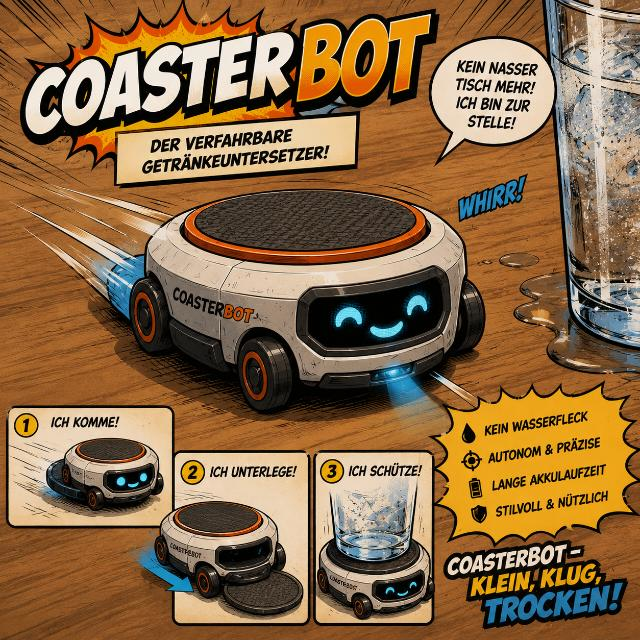
\includegraphics[width=0.38\textwidth]{coasterbot.png}} \\[1em]

\vspace{4em}

    {\normalsize
\begin{tabular}{ll}
Dennis Borutta, B. Eng & dennis.borutta@outlook.com\\
Stefan Etringer, B. Eng & mail@stefan.works\\
Gereon Such, M. Sc. & gereonsuch@gmail.com\\
\end{tabular}
    }
  \end{center}
\end{titlepage}

\section*{Versionshistorie}
\begin{tabular}{@{}p{1.6cm}p{2.4cm}p{3.0cm}>{\raggedright\arraybackslash}p{7.0cm}@{}}
\toprule
\textbf{Version} & \textbf{Datum} & \textbf{Bearbeiter} & \textbf{Änderung}\\
\midrule
1 & 28.08.2026 & Such & Erstfassung, zunächst nur Elektronik \\
\bottomrule
\end{tabular}
\clearpage


\section{Allgemeines}

Dieses Dokument beschreibt die Schritte zum Aufbau eines funktionsfähigen Prototypen aus den Komponenten laut Stückliste. Die Einzelkomponenten sowie die Firmware werden in separaten Dokumenten beschrieben. 

Folgende Fähigkeiten und Werkzeuge werden für die Montage vorausgesetzt:

\begin{enumerate}
\item 3D Drucker für den Druck des Chassis
\item Grundlegende Erfahrung im Umgang mit dem genutzten 3D Drucker
\item Montagewerkzeug für die Chassis Schrauben
\item Grundlegende Fähigkeiten in der Feinmechanik
\item Lötwerkzeug
\item Fortgeschrittene Fähigkeiten im Umgang mit Elektronik und Lochrasterplatinenmontage

\end{enumerate}


Abbildung \ref{fig:schematic} zeigt die Gesamtschaltung der Elektronik. Die Komponenten sind weitestgehend als Dev-Boards integriert und auch als solche im Schaltplan aufgeführt. Das Dokument BOM beschreibt die jeweiligen Komponenten sowie die Bezugsquelle. 

\begin{landscape}
\begin{figure}
    \centering
    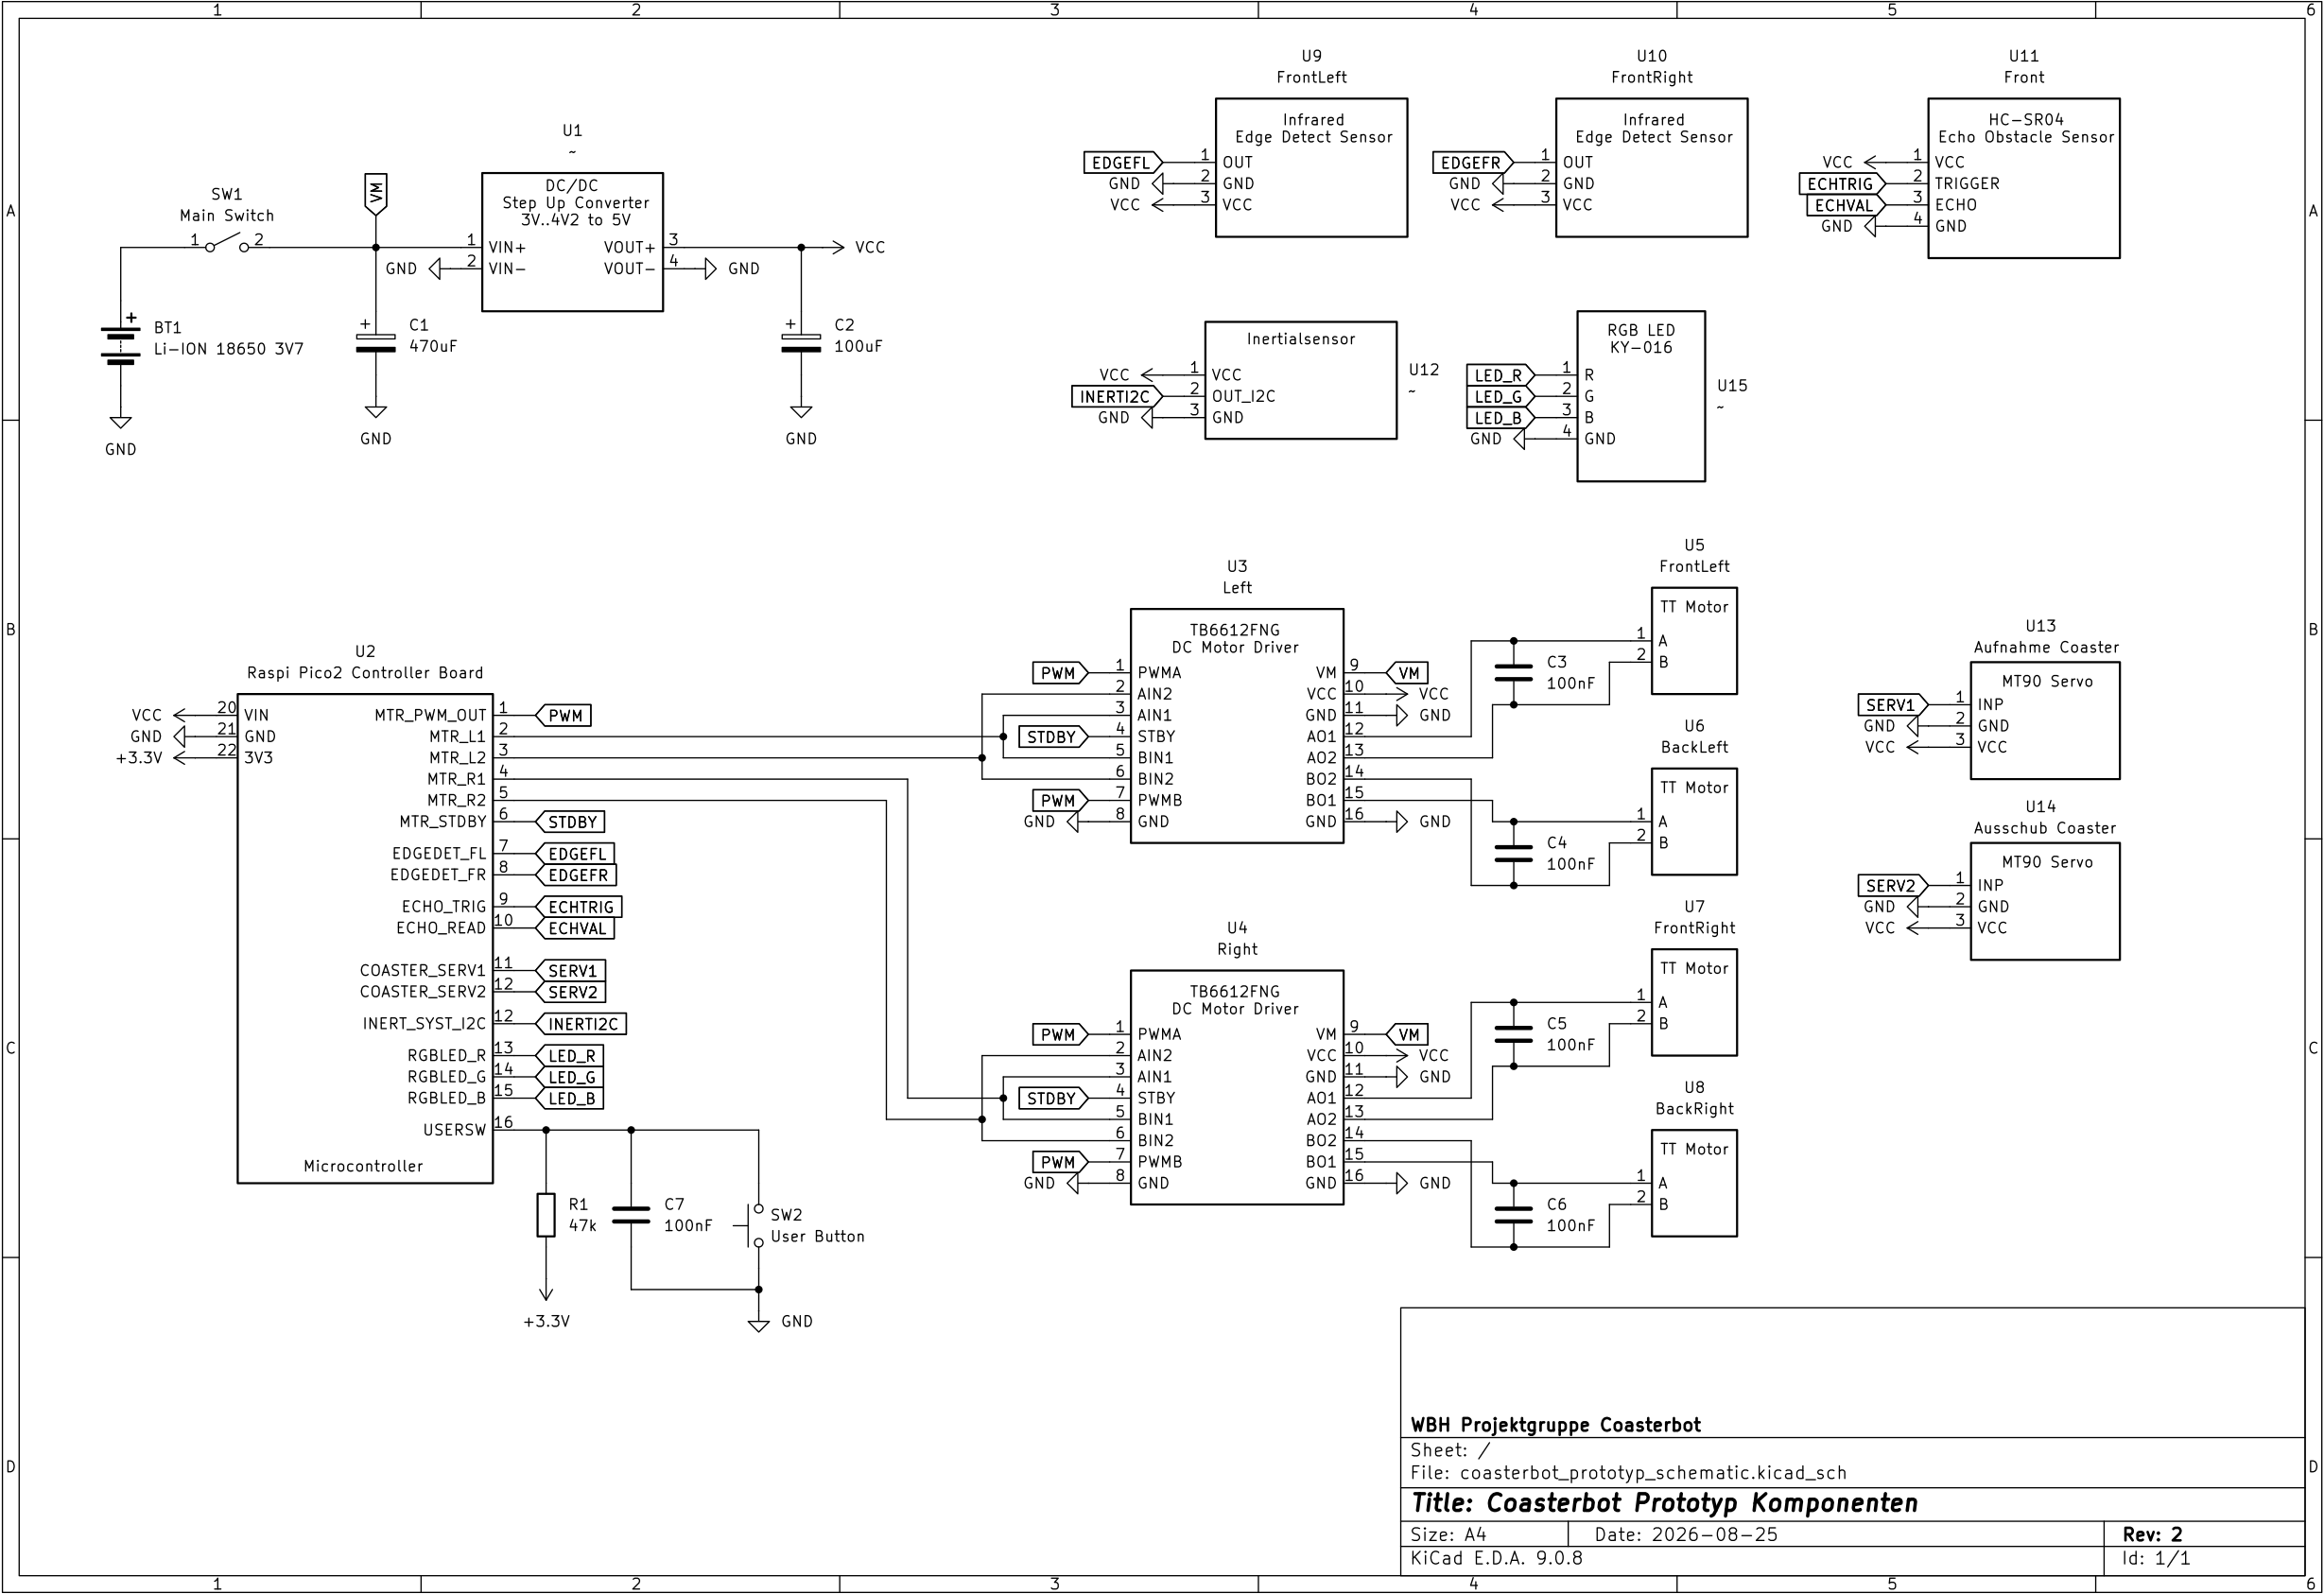
\includegraphics[width=\linewidth]{schematic.png}
    \caption{Gesamtschaltung}
    \label{fig:schematic}
\end{figure}
\end{landscape}


\FloatBarrier

\section{Montage}

\subsection{3D Druck des Chassis}

Das Chassis des Coasterbots wurde mit FreeCAD entwickelt und wird sowohl als FreeCAD Projekt als auch fertigen \texttt{.stl} Dateien im Github Repository \footnote{\url{https://github.com/Project-CoasterBot/coasterbot/tree/main}} bereitgestellt. Für den einfachen 3D Druck genügen hier die \texttt{.stl} Dateien. 

Diese müssen heruntergeladen und dann entsprechend des genutzten 3D Druckers geslicet werden, dazu kann z.B. der Orca-Slicer \footnote{\url{https://www.orcaslicer.com/}} genutzt werden, welcher eine Vielzahl von 3D Druckern und Interfaces zu diesen Druckern unterstützt. Nach dem Slicen können die Komponenten entweder über eine Netzwerkschnittstelle oder Peripherie Medium wie SD Karte an den 3D Drucker übertragen werden. Insgesamt wird für das Projekt ca. 500g PLA Medium benötigt, es können aber auch andere Materialien wie PETG verwendet werden. 

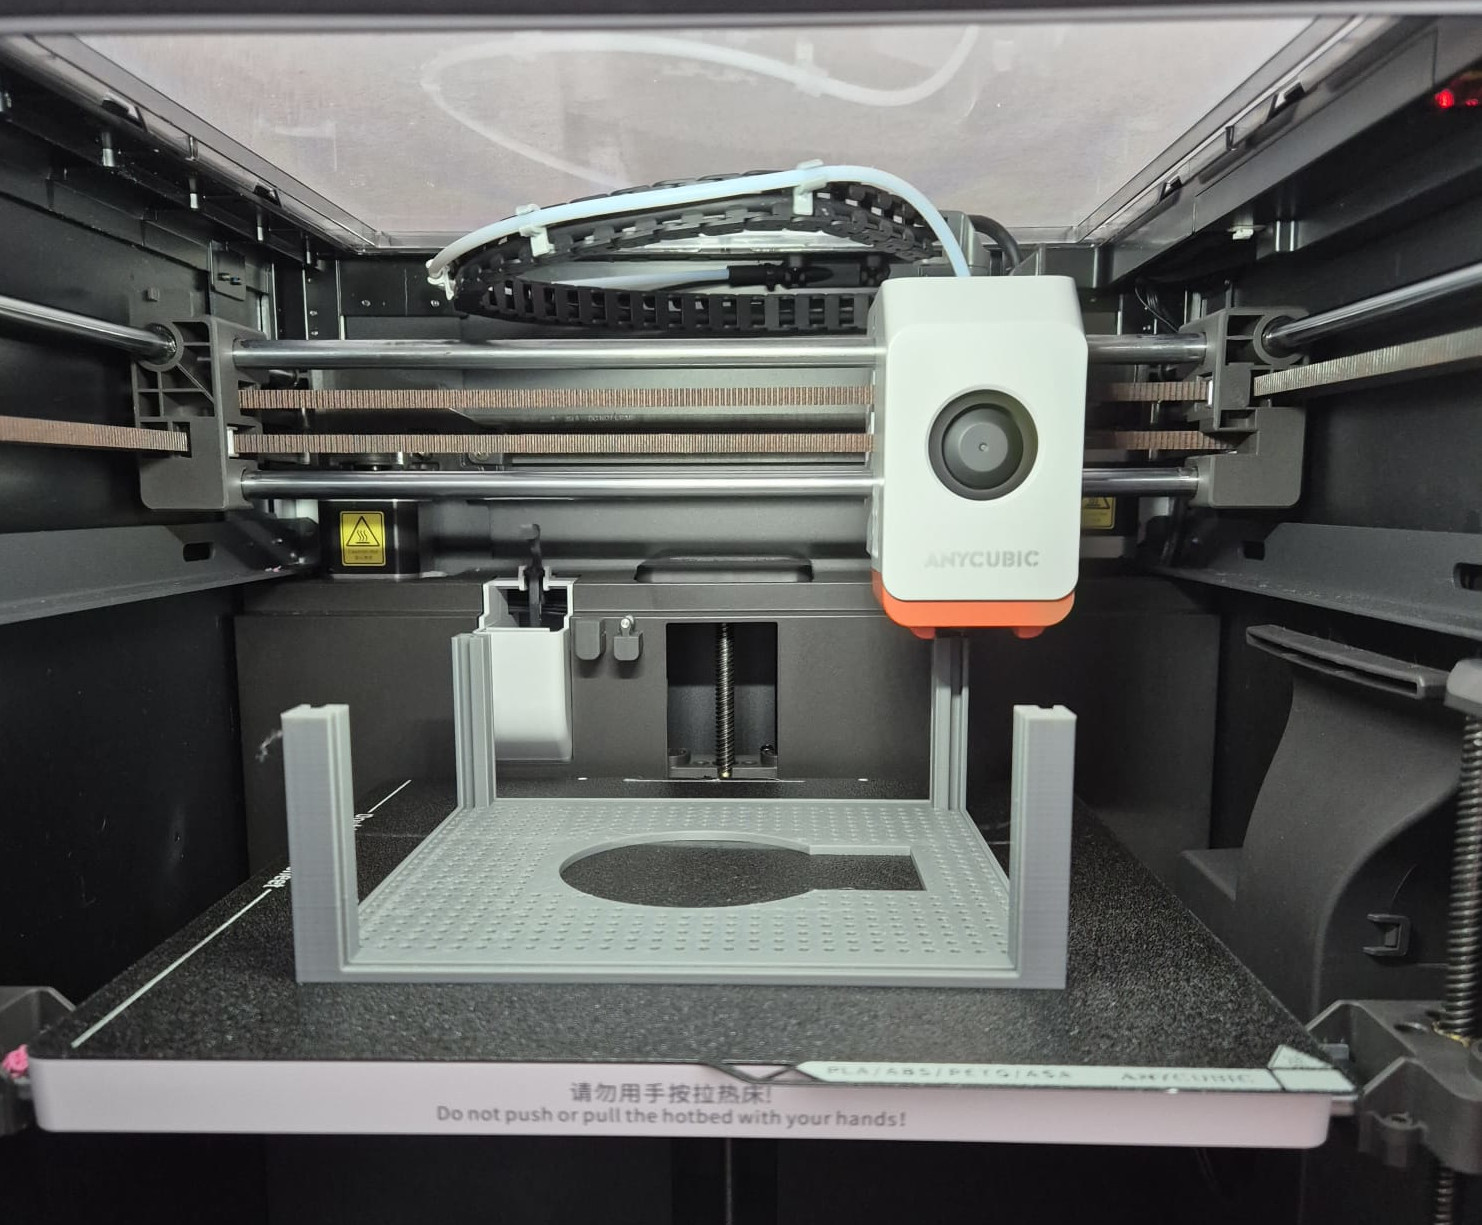
\includegraphics[scale=1.]{montage_gereon/IMG-20260912-WA0000.jpg}



%\subsection{Coaster montieren}
%TODO Magneten einführen
%TODO Coaster verschließen

\subsection{Chassis Grundgerüst montieren}

Zunächst wird hier das Coaster Reservoir auf die Grundplatte montiert:

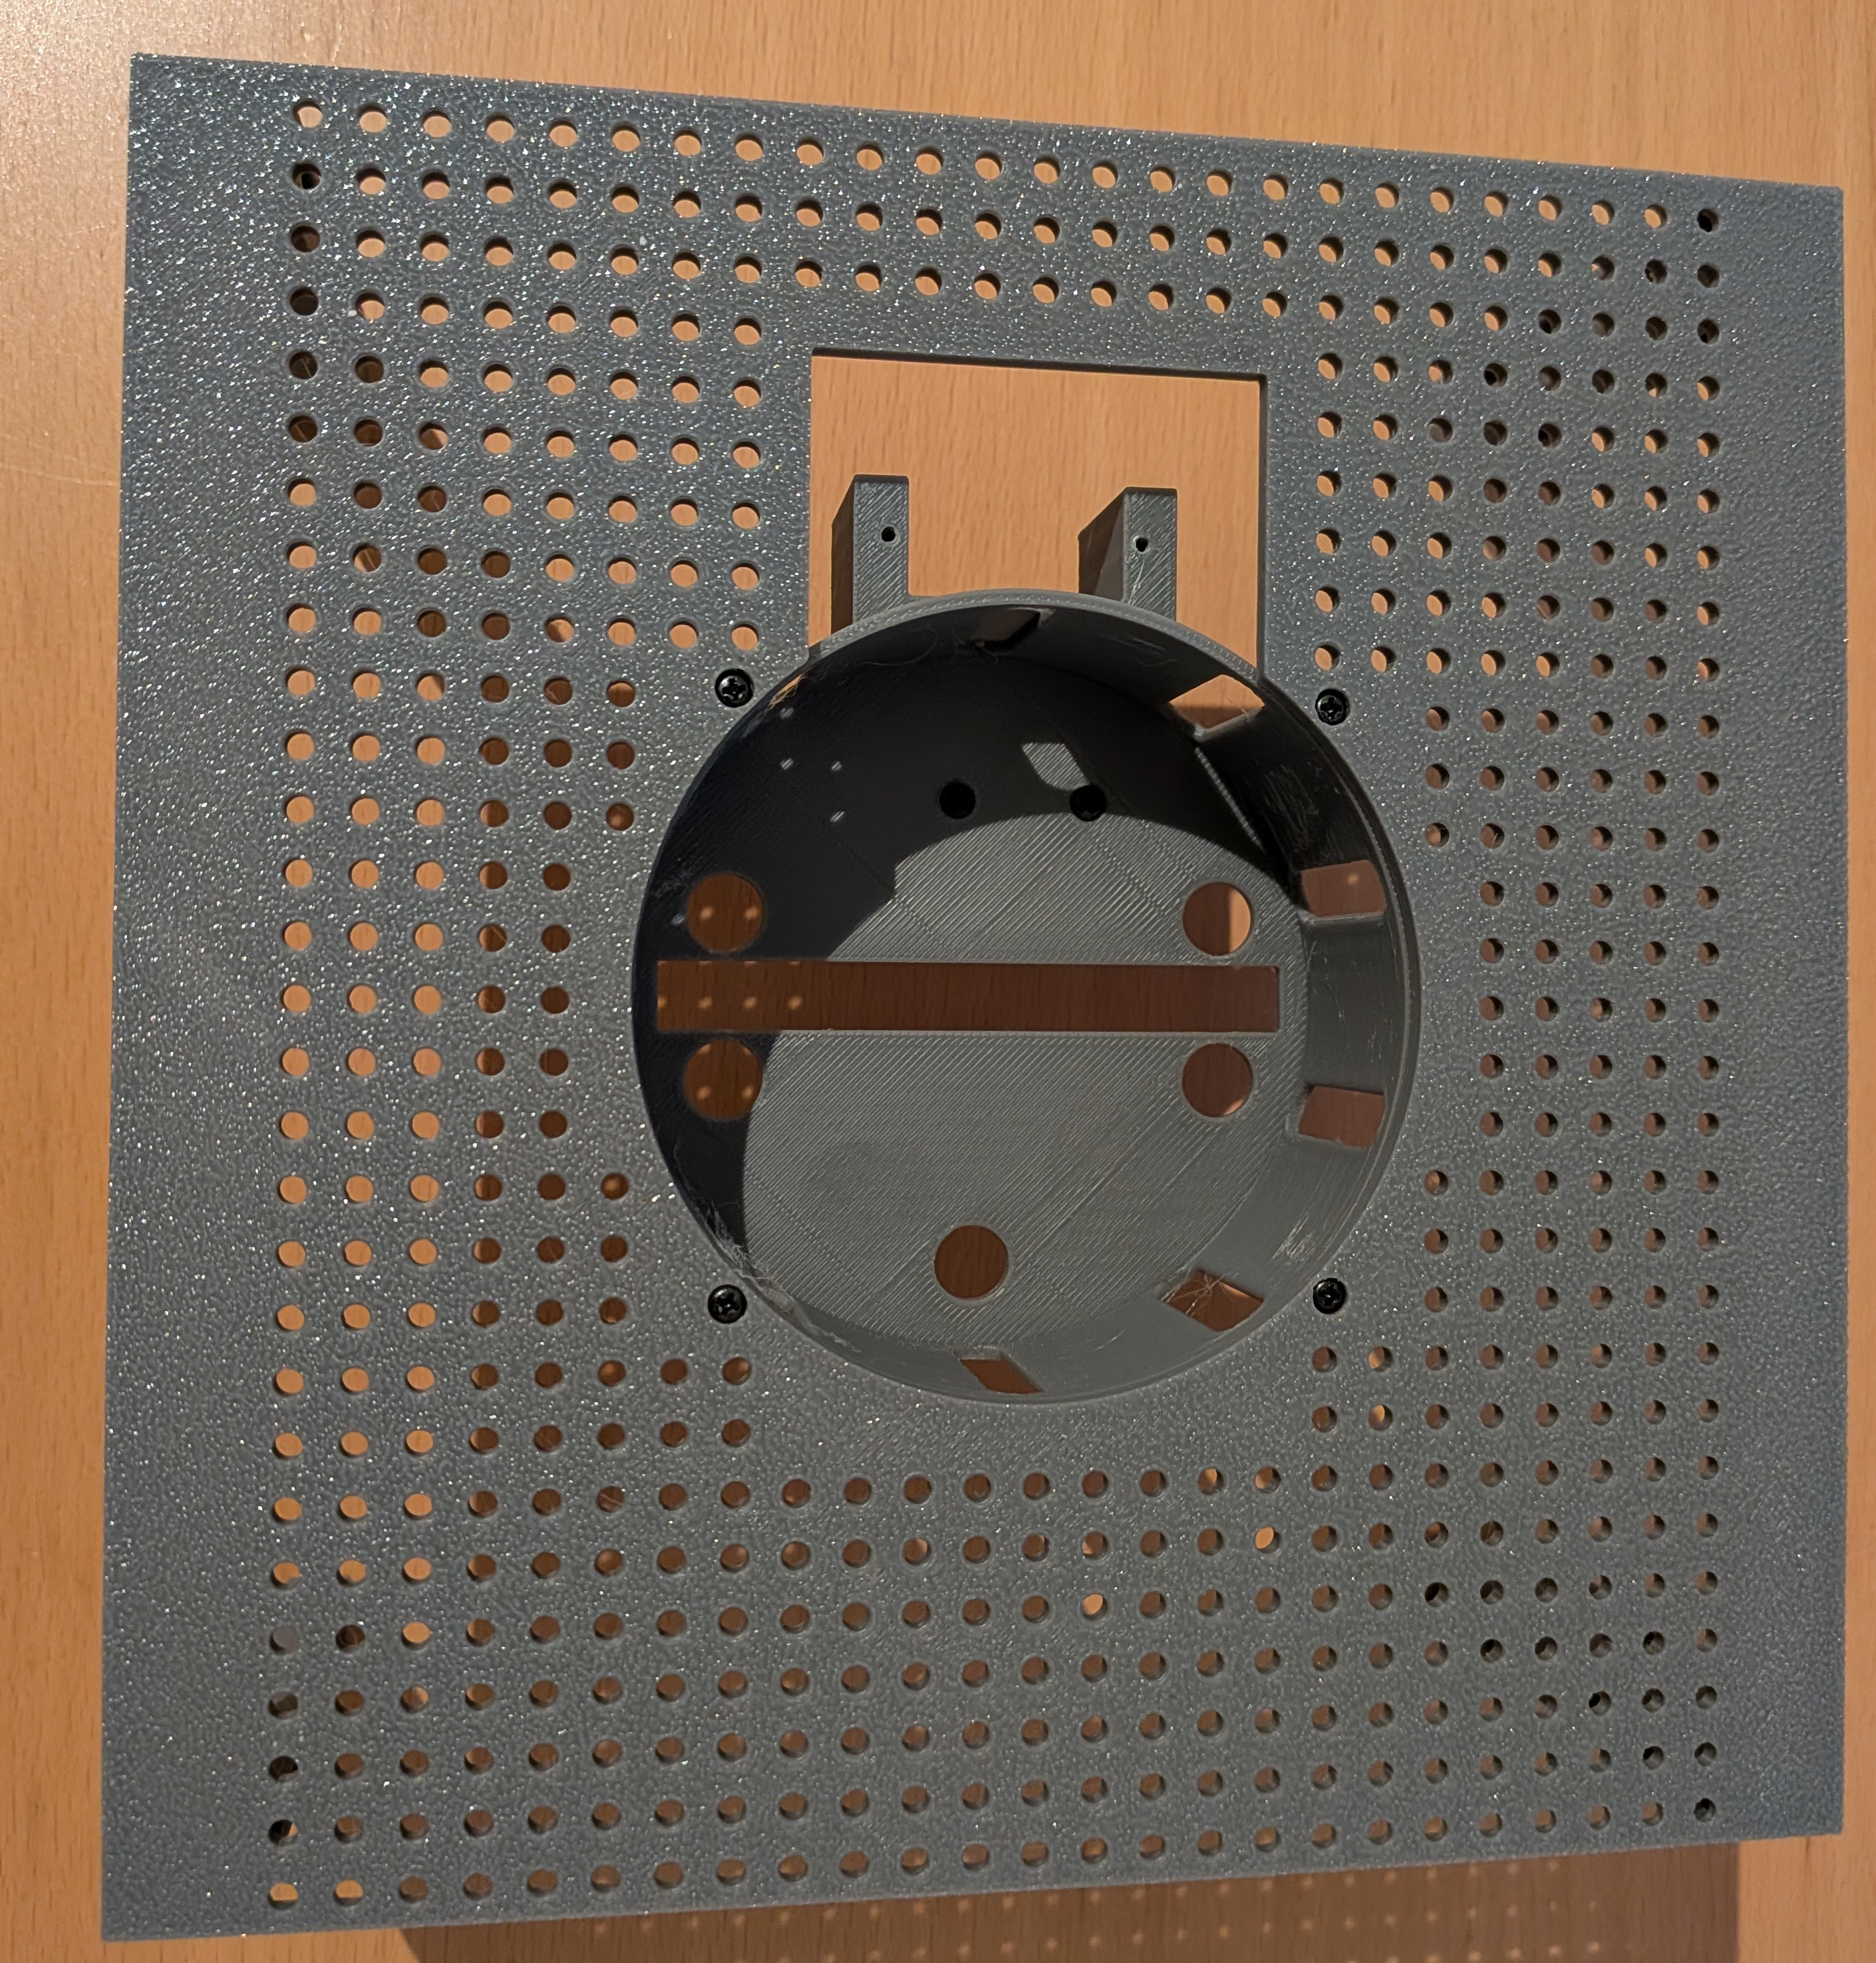
\includegraphics[scale=0.08]{montage_gereon/basis_konstrukt/PXL_20260909_073241241.jpg}

Anschließend werden die Träger an den Ecken angebracht:

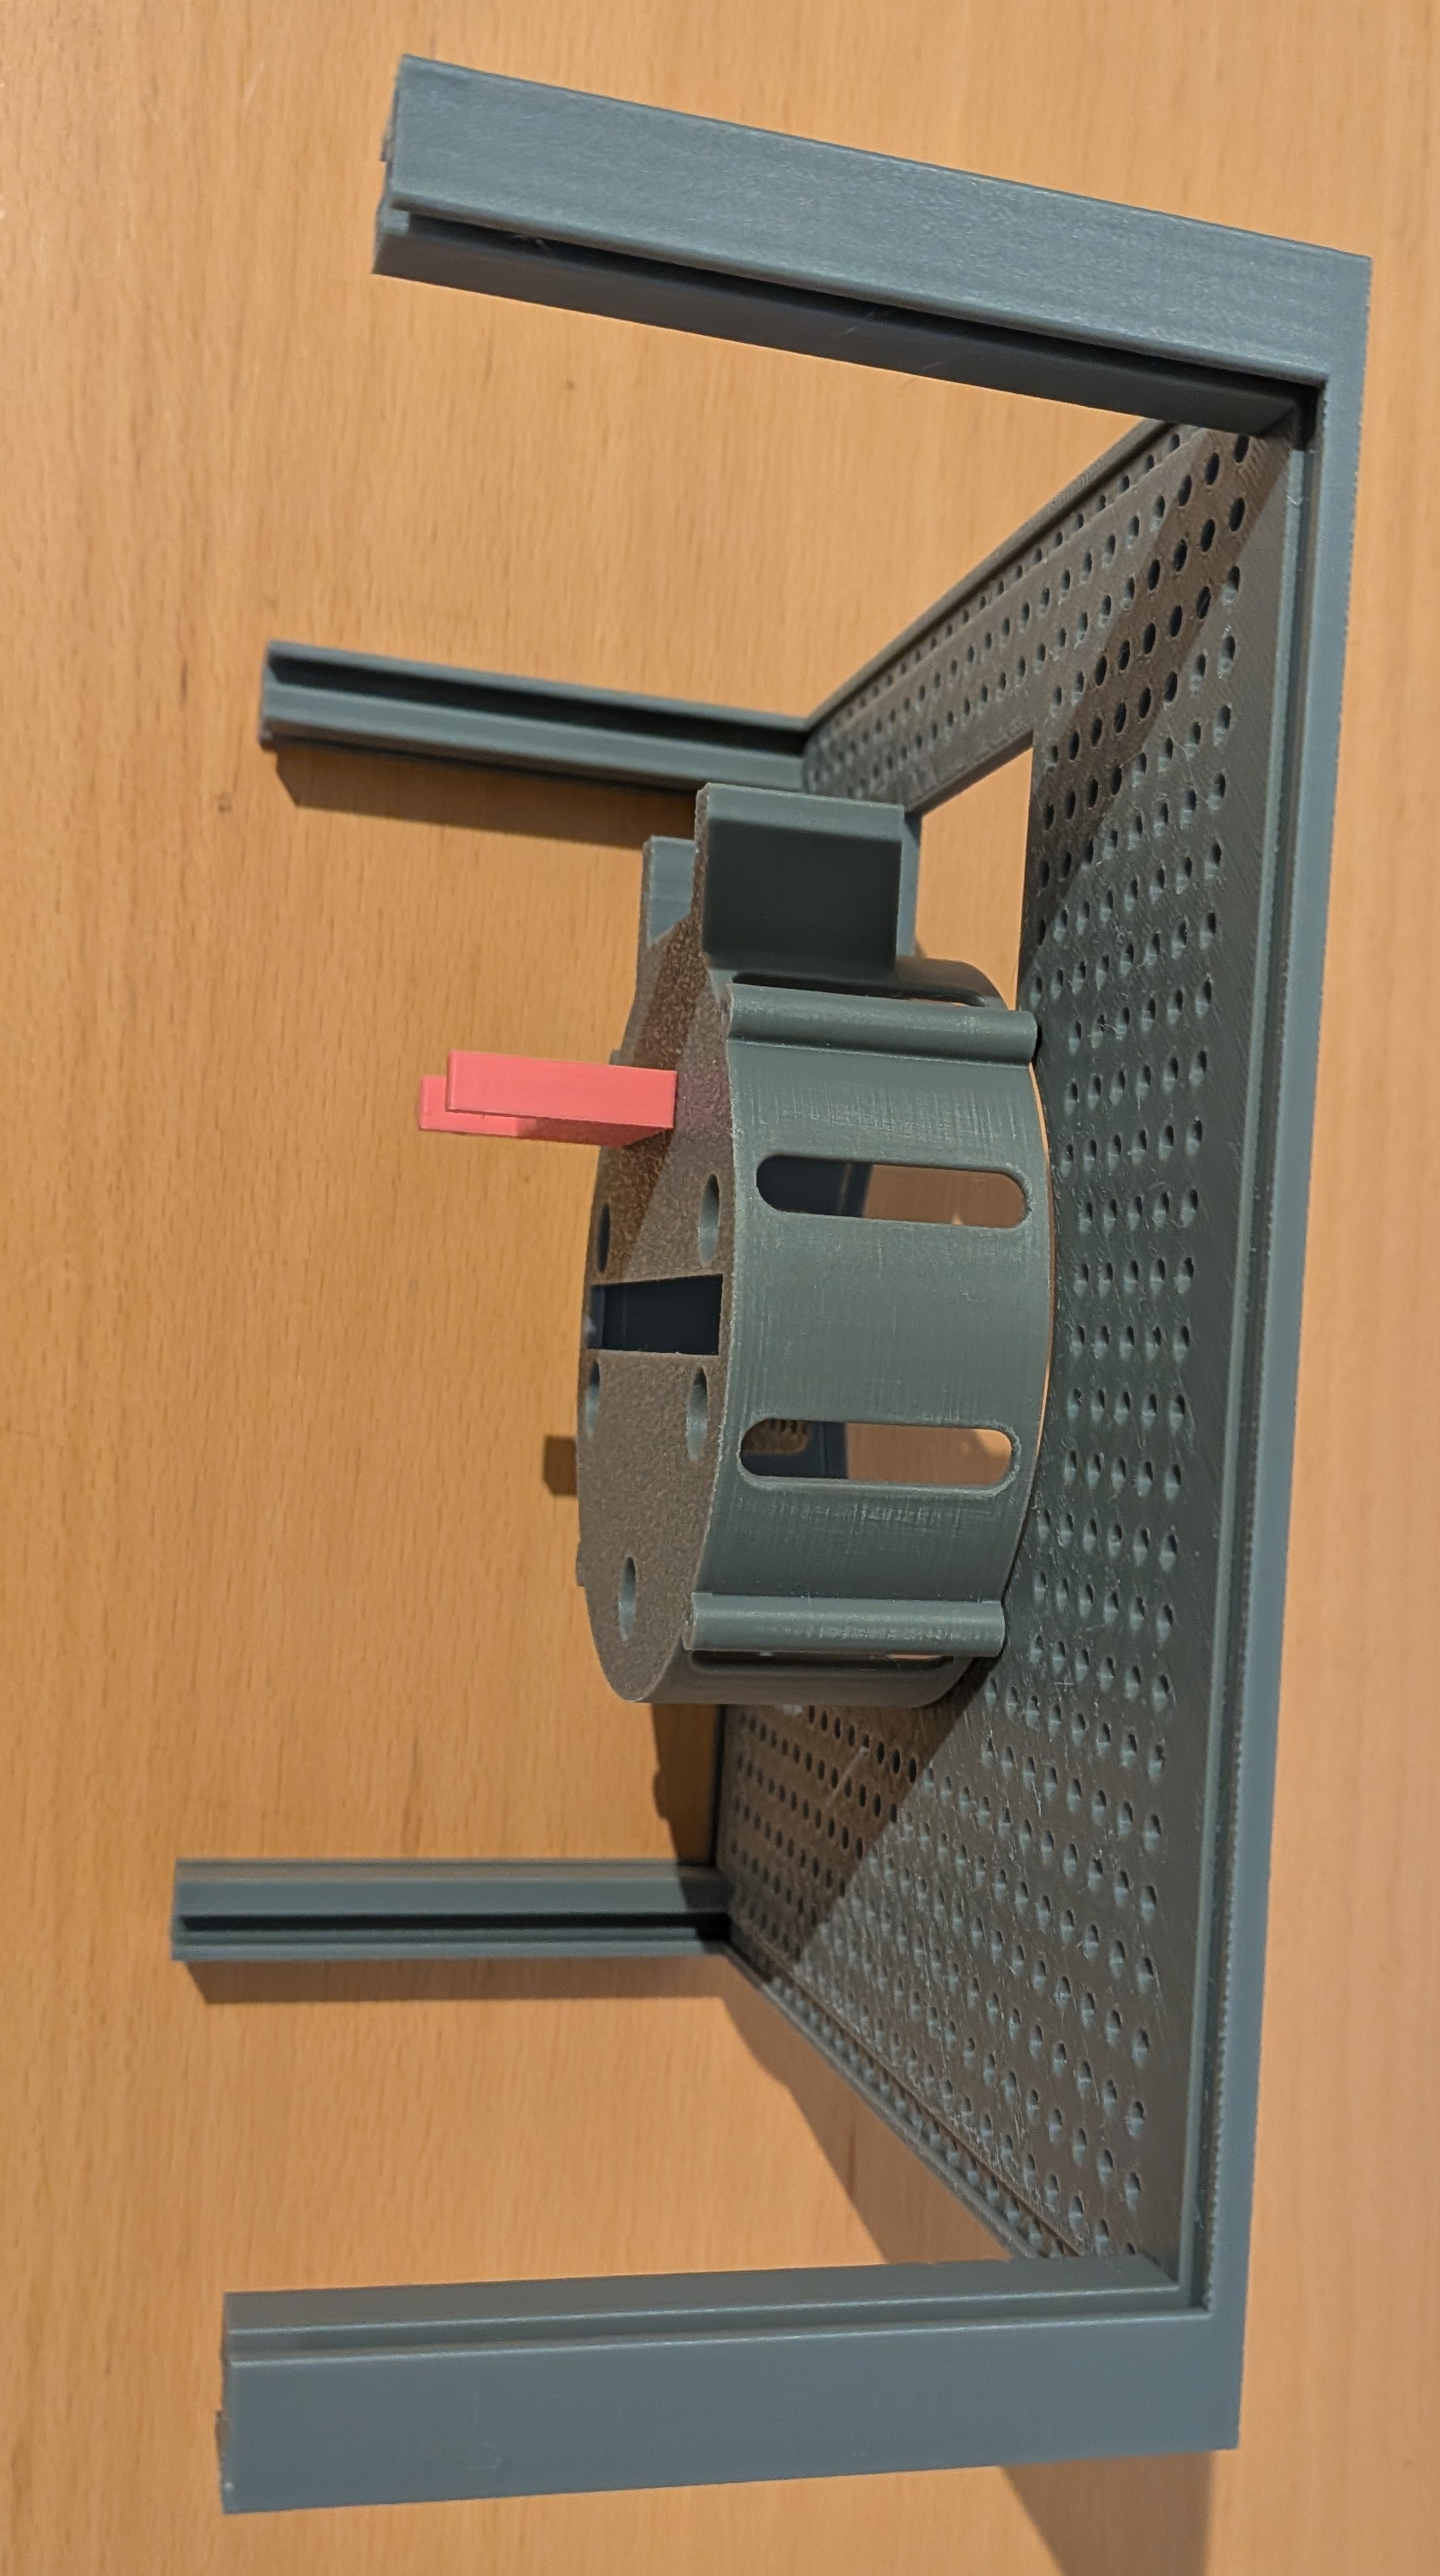
\includegraphics[scale=0.08]{montage_gereon/basis_konstrukt/PXL_20260909_073304730.jpg}
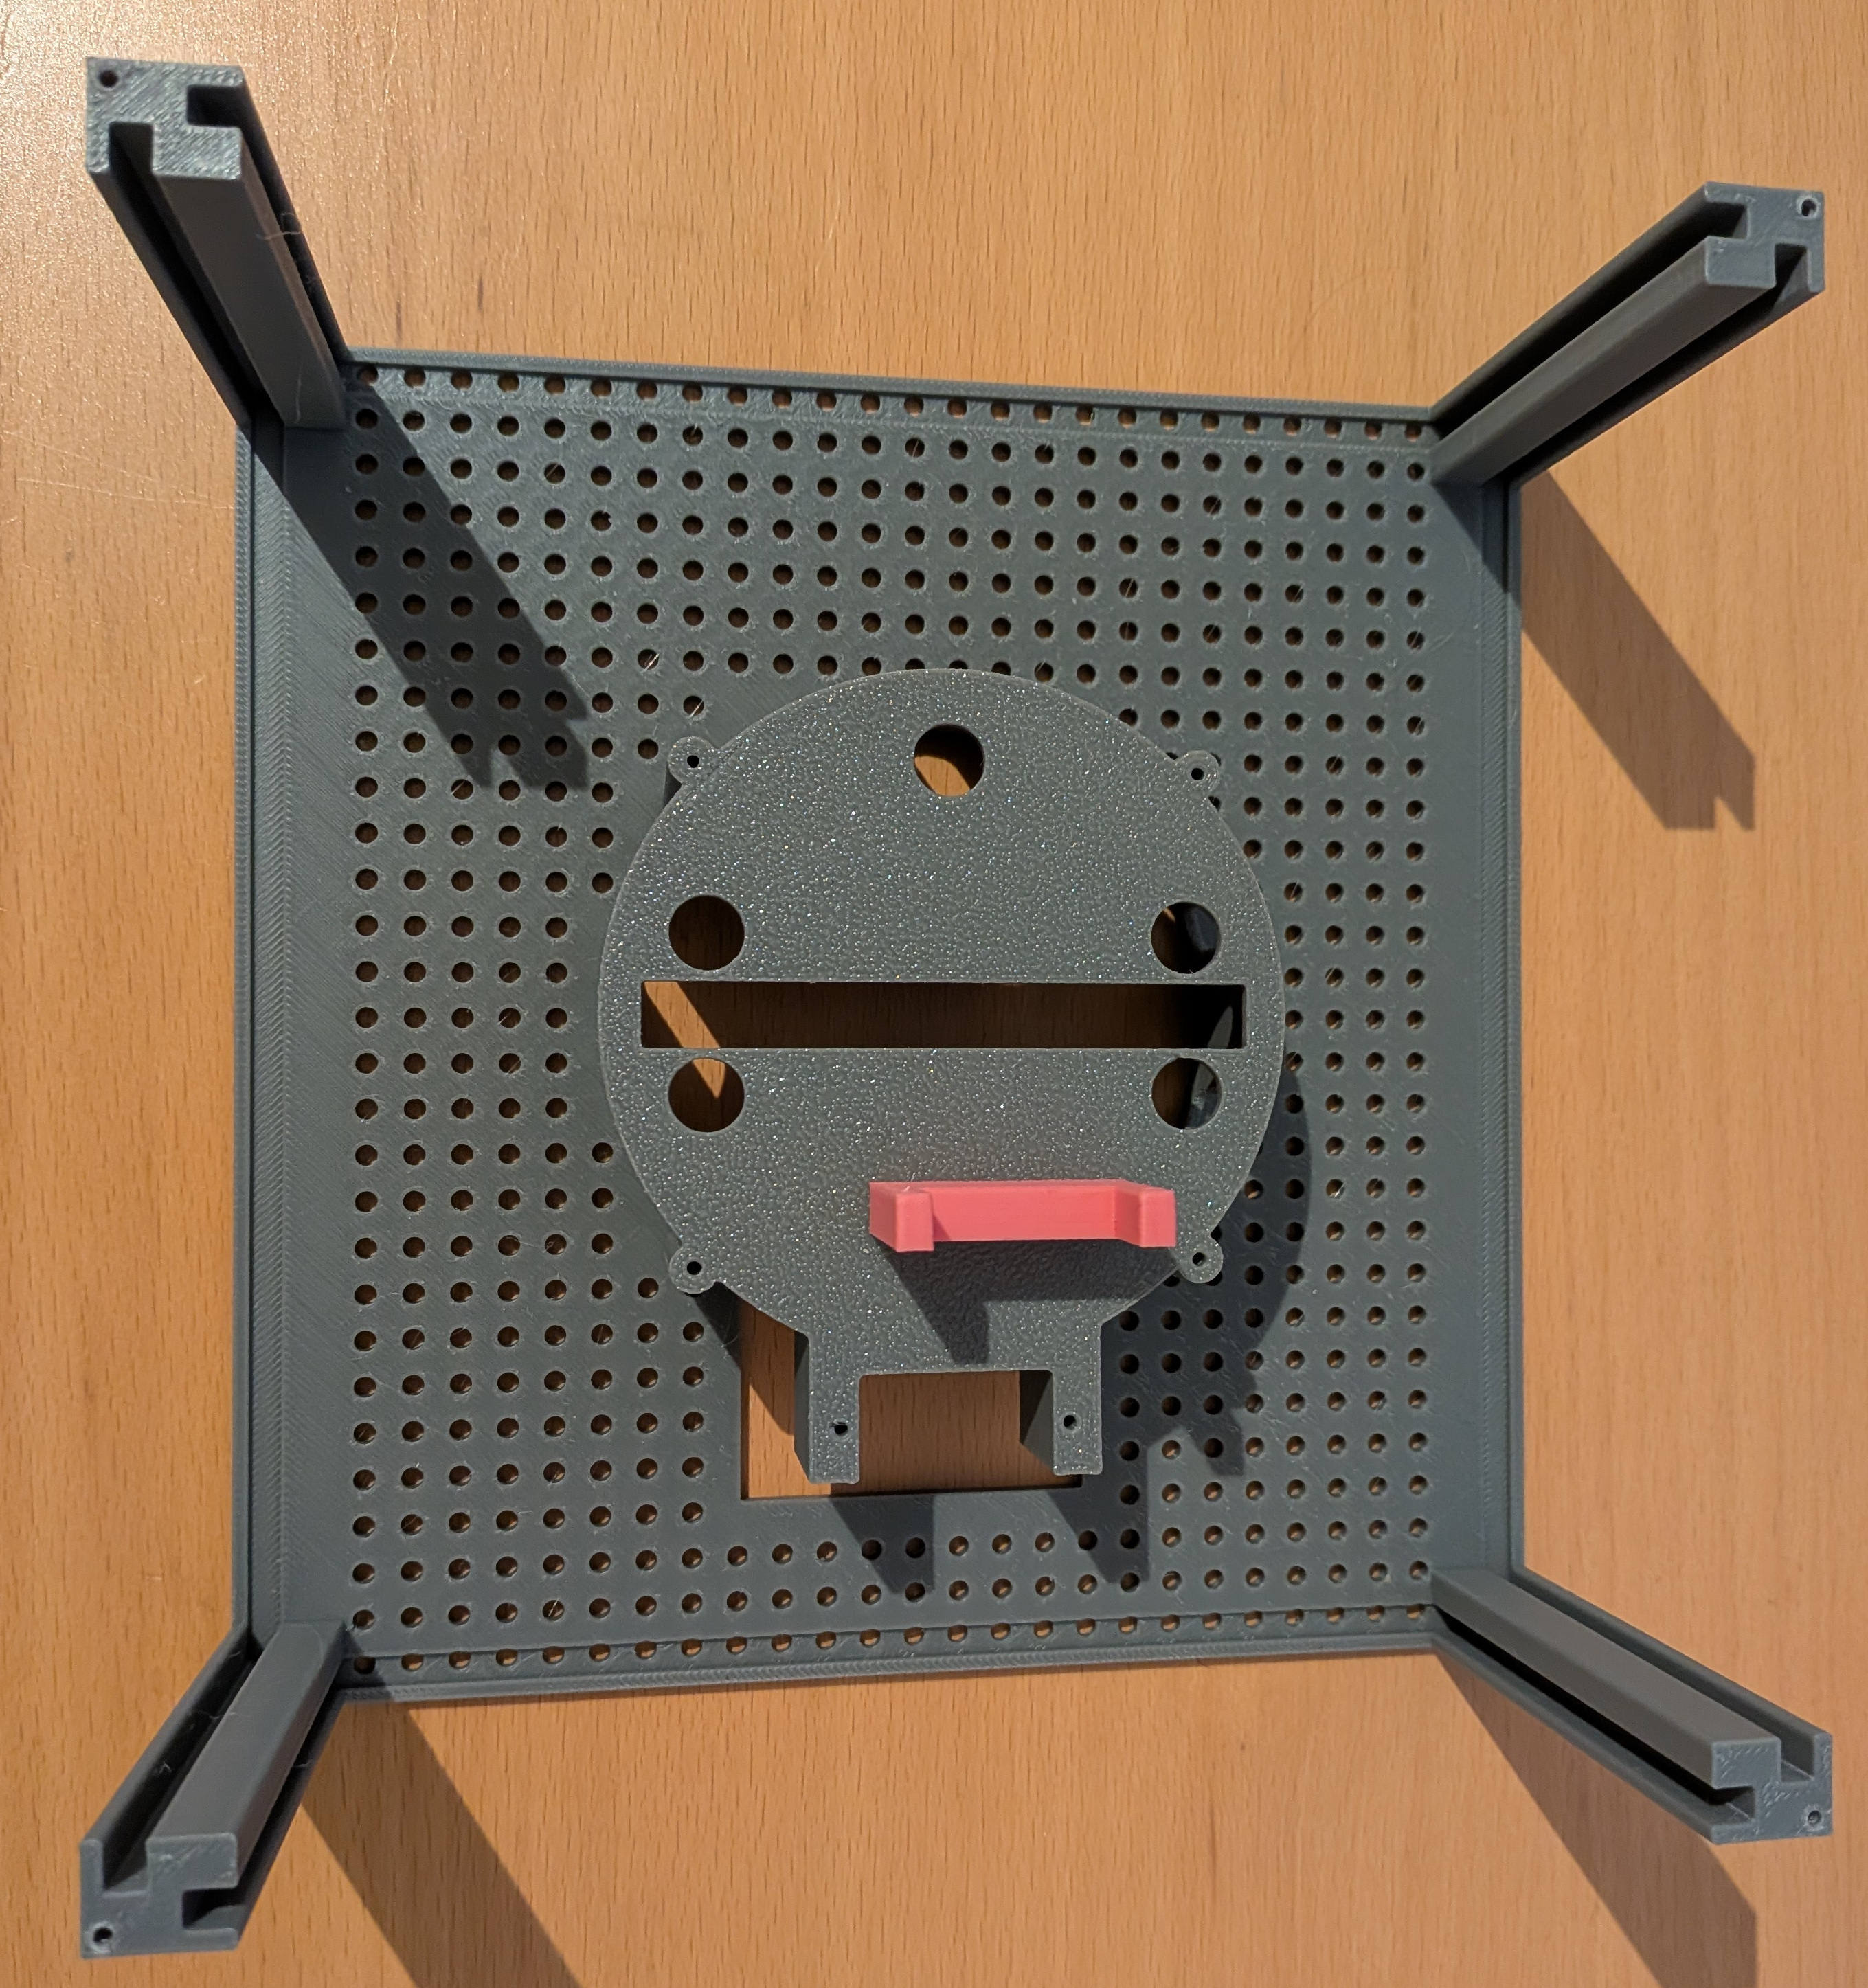
\includegraphics[scale=0.08]{montage_gereon/basis_konstrukt/PXL_20260909_073227706.jpg}



\subsection{Coastermechanismus Montieren}

Nun wird der Mechanismus zur Coasteraufnahme montiert:

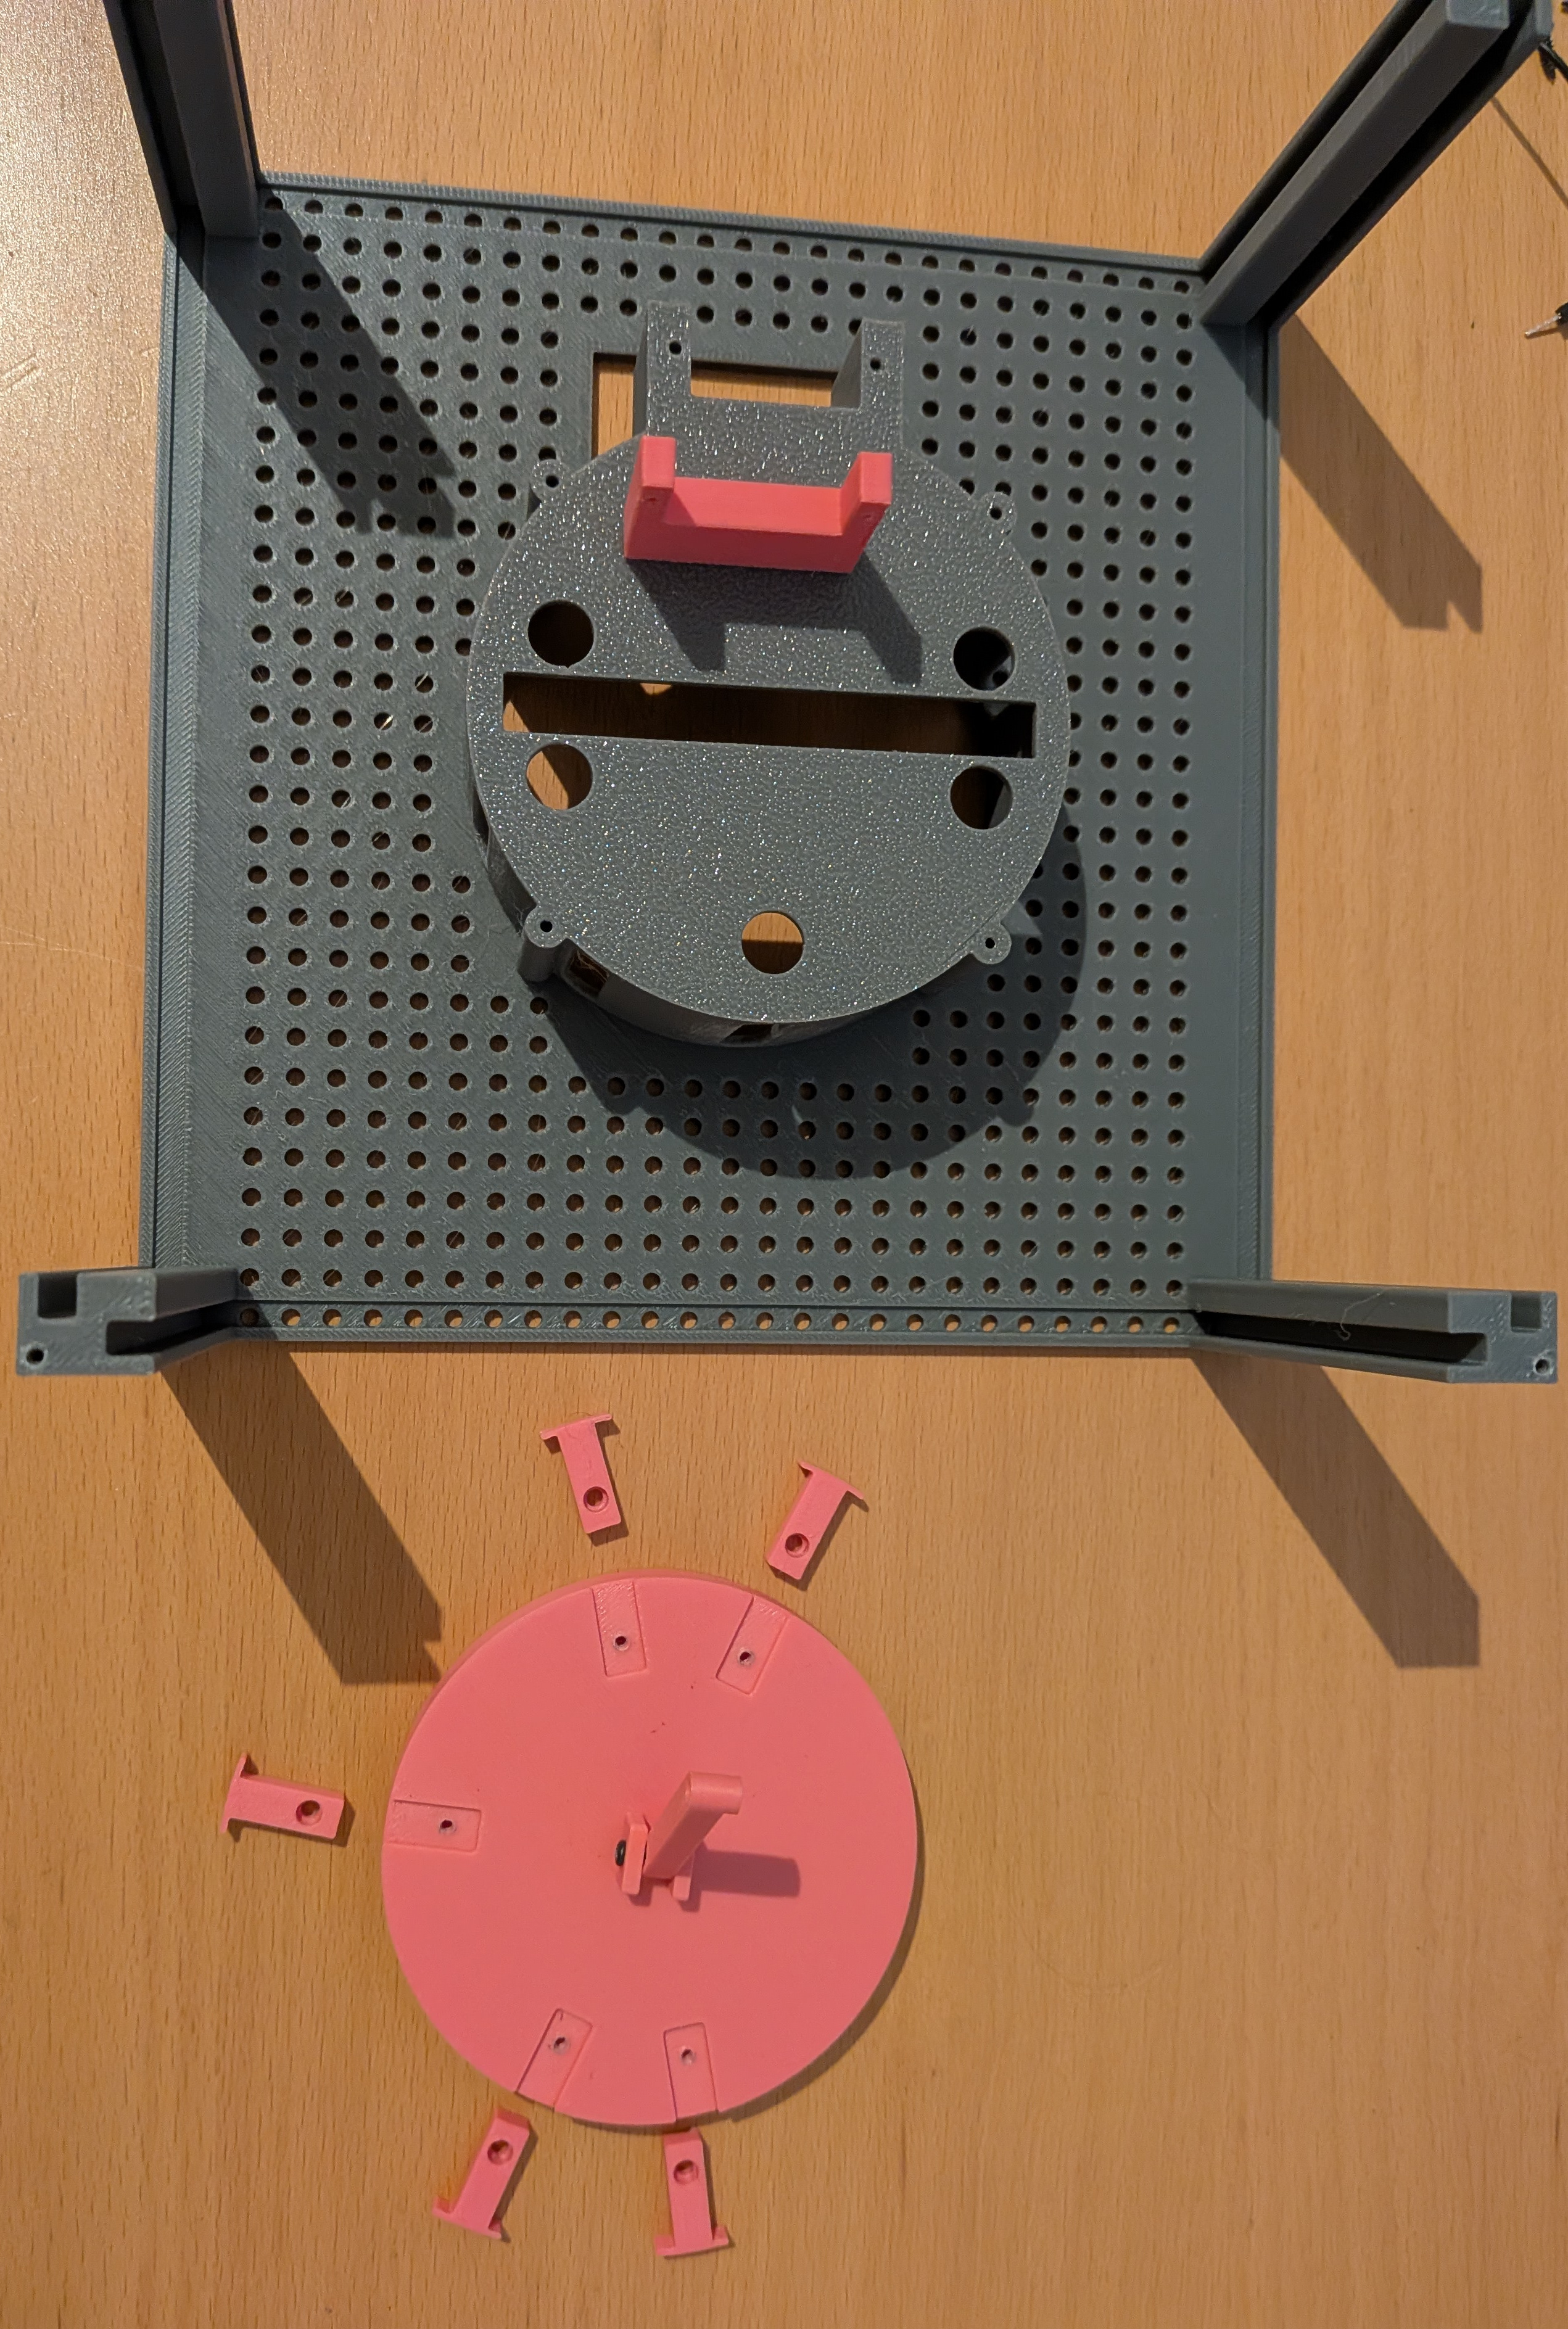
\includegraphics[scale=0.08]{montage_gereon/basis_konstrukt/PXL_20260909_073450774.jpg}

Dazu muss der Träger zunächst ohne die Führungsachsen in die Coasteraufnahme eingelegt werden, anschließend werden die Führungsachsen von außen auf der Coasteraufnahme verschraubt. Die Coasteraufnahme hat dazu auf der Oberseite Löcher zum durchführen eines Schraubenziehers. 

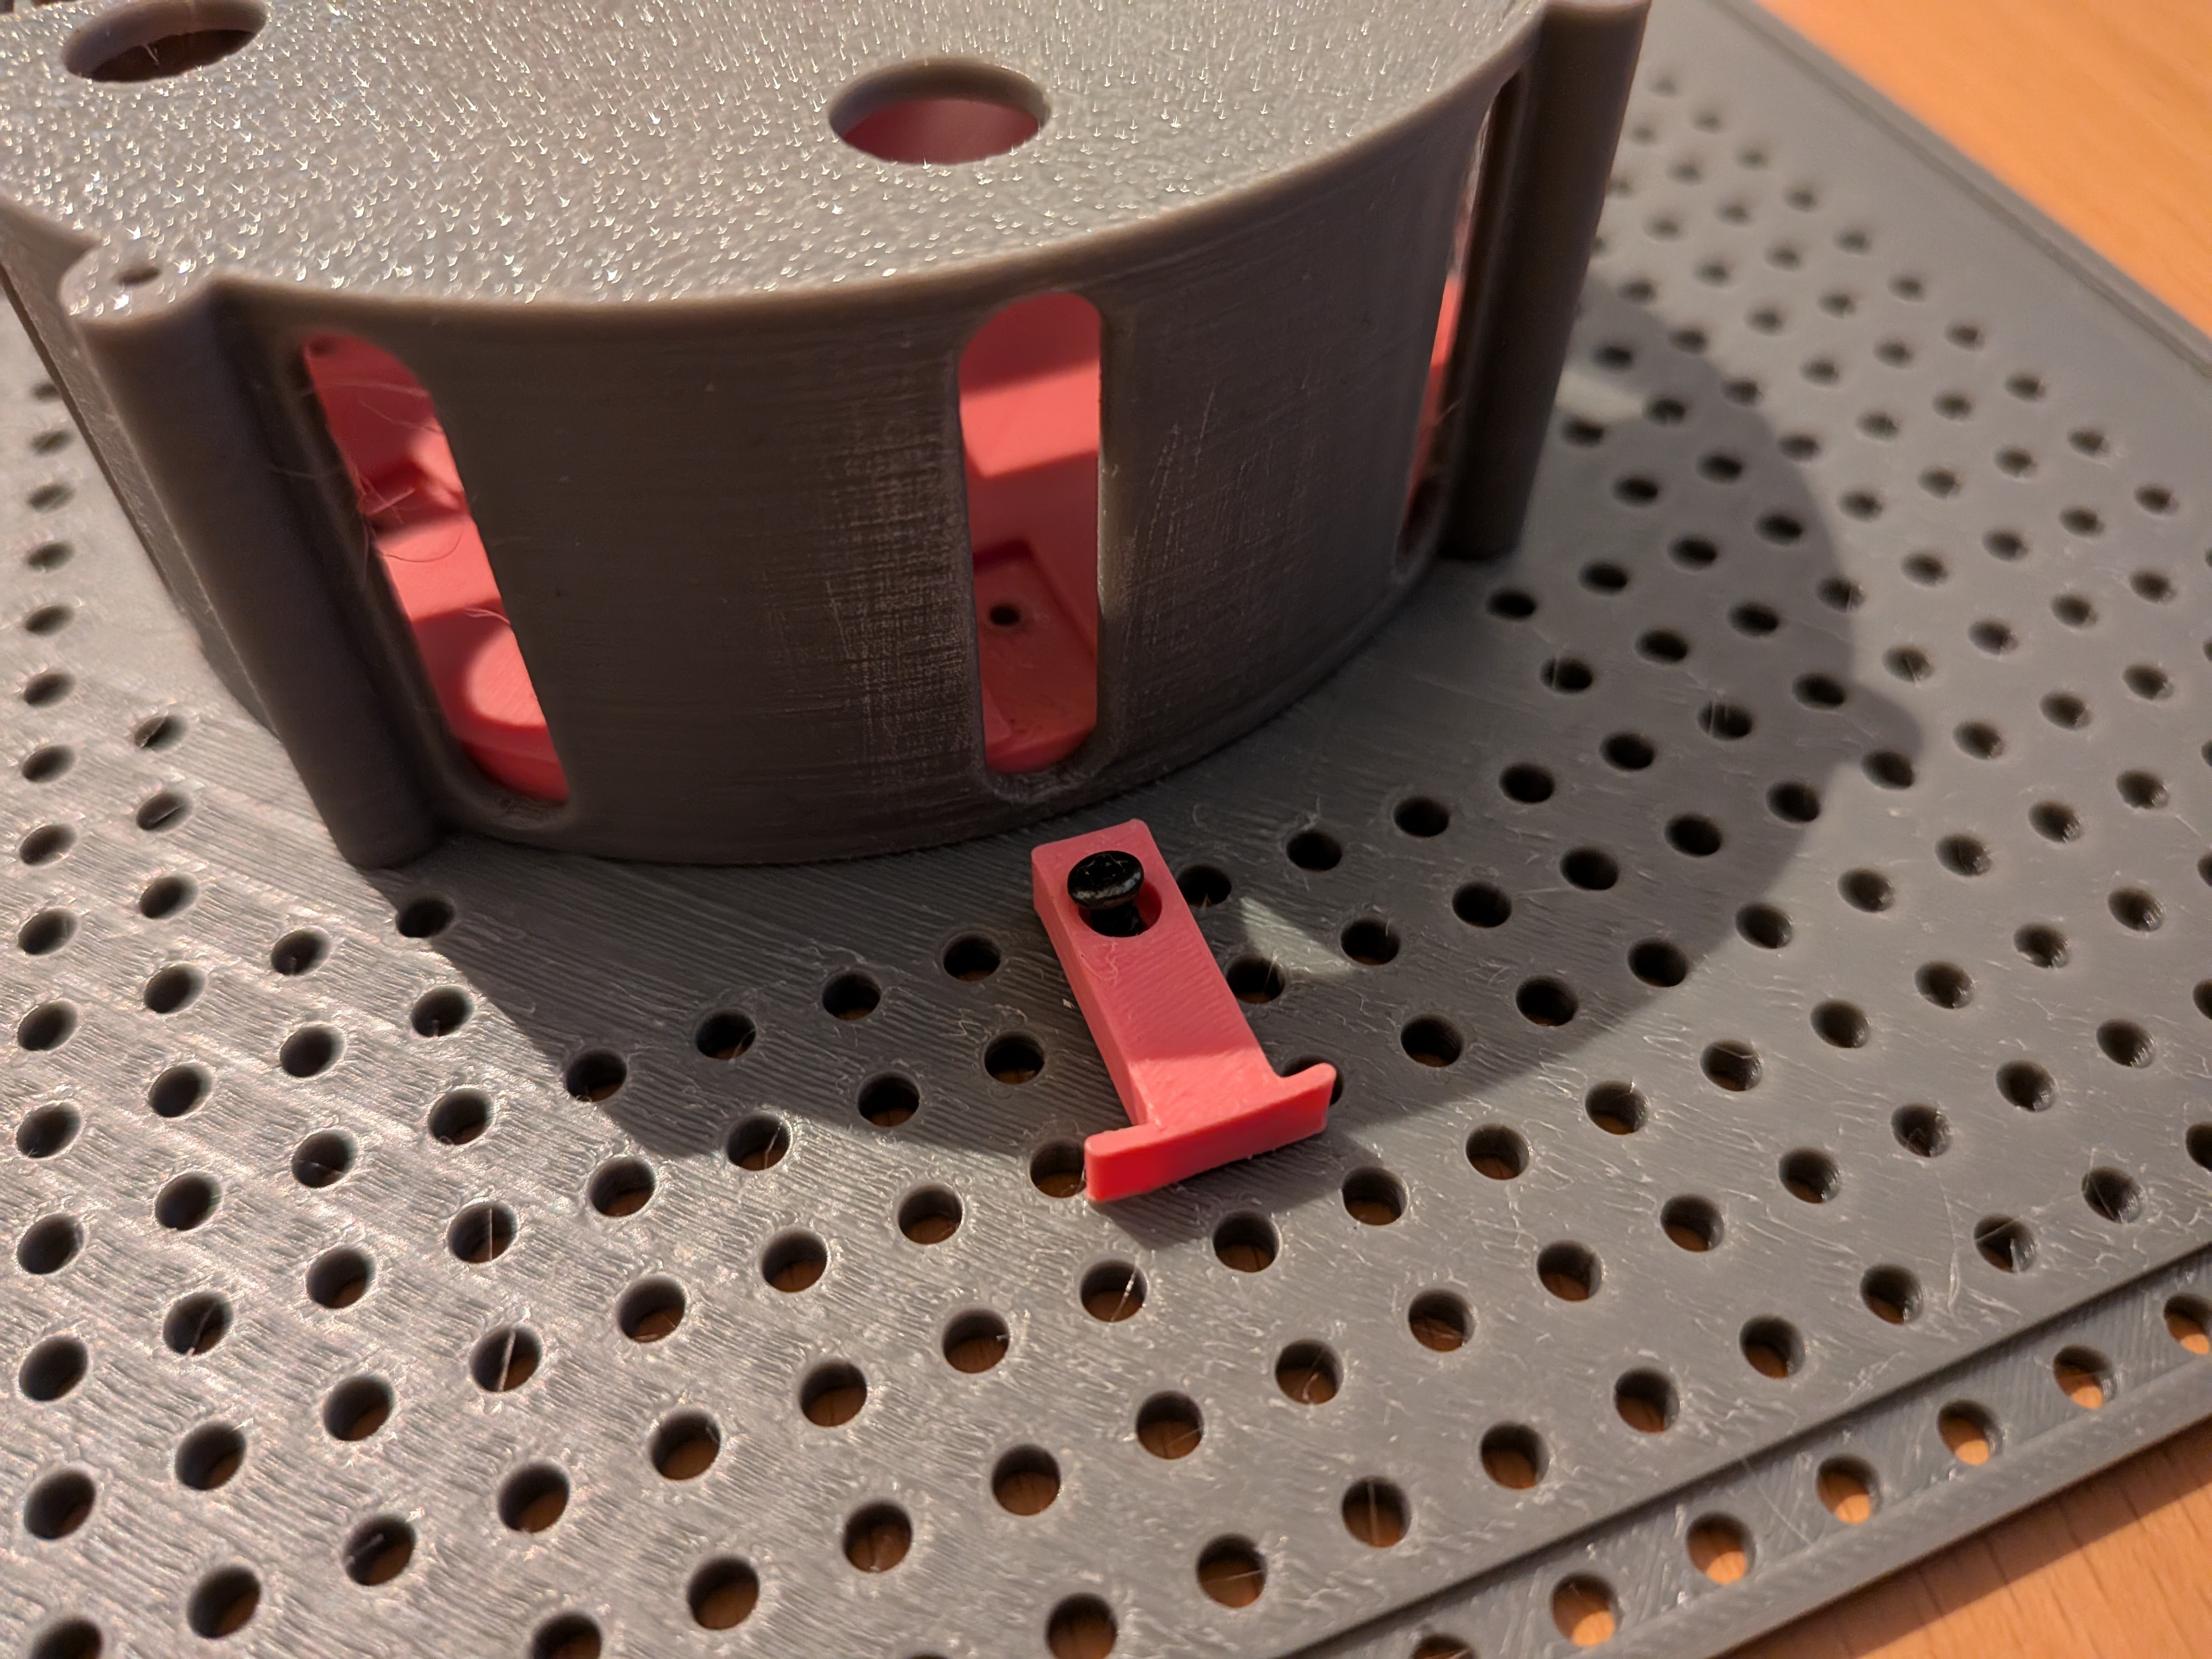
\includegraphics[scale=0.06]{montage_gereon/basis_konstrukt/PXL_20260909_073617594.jpg}
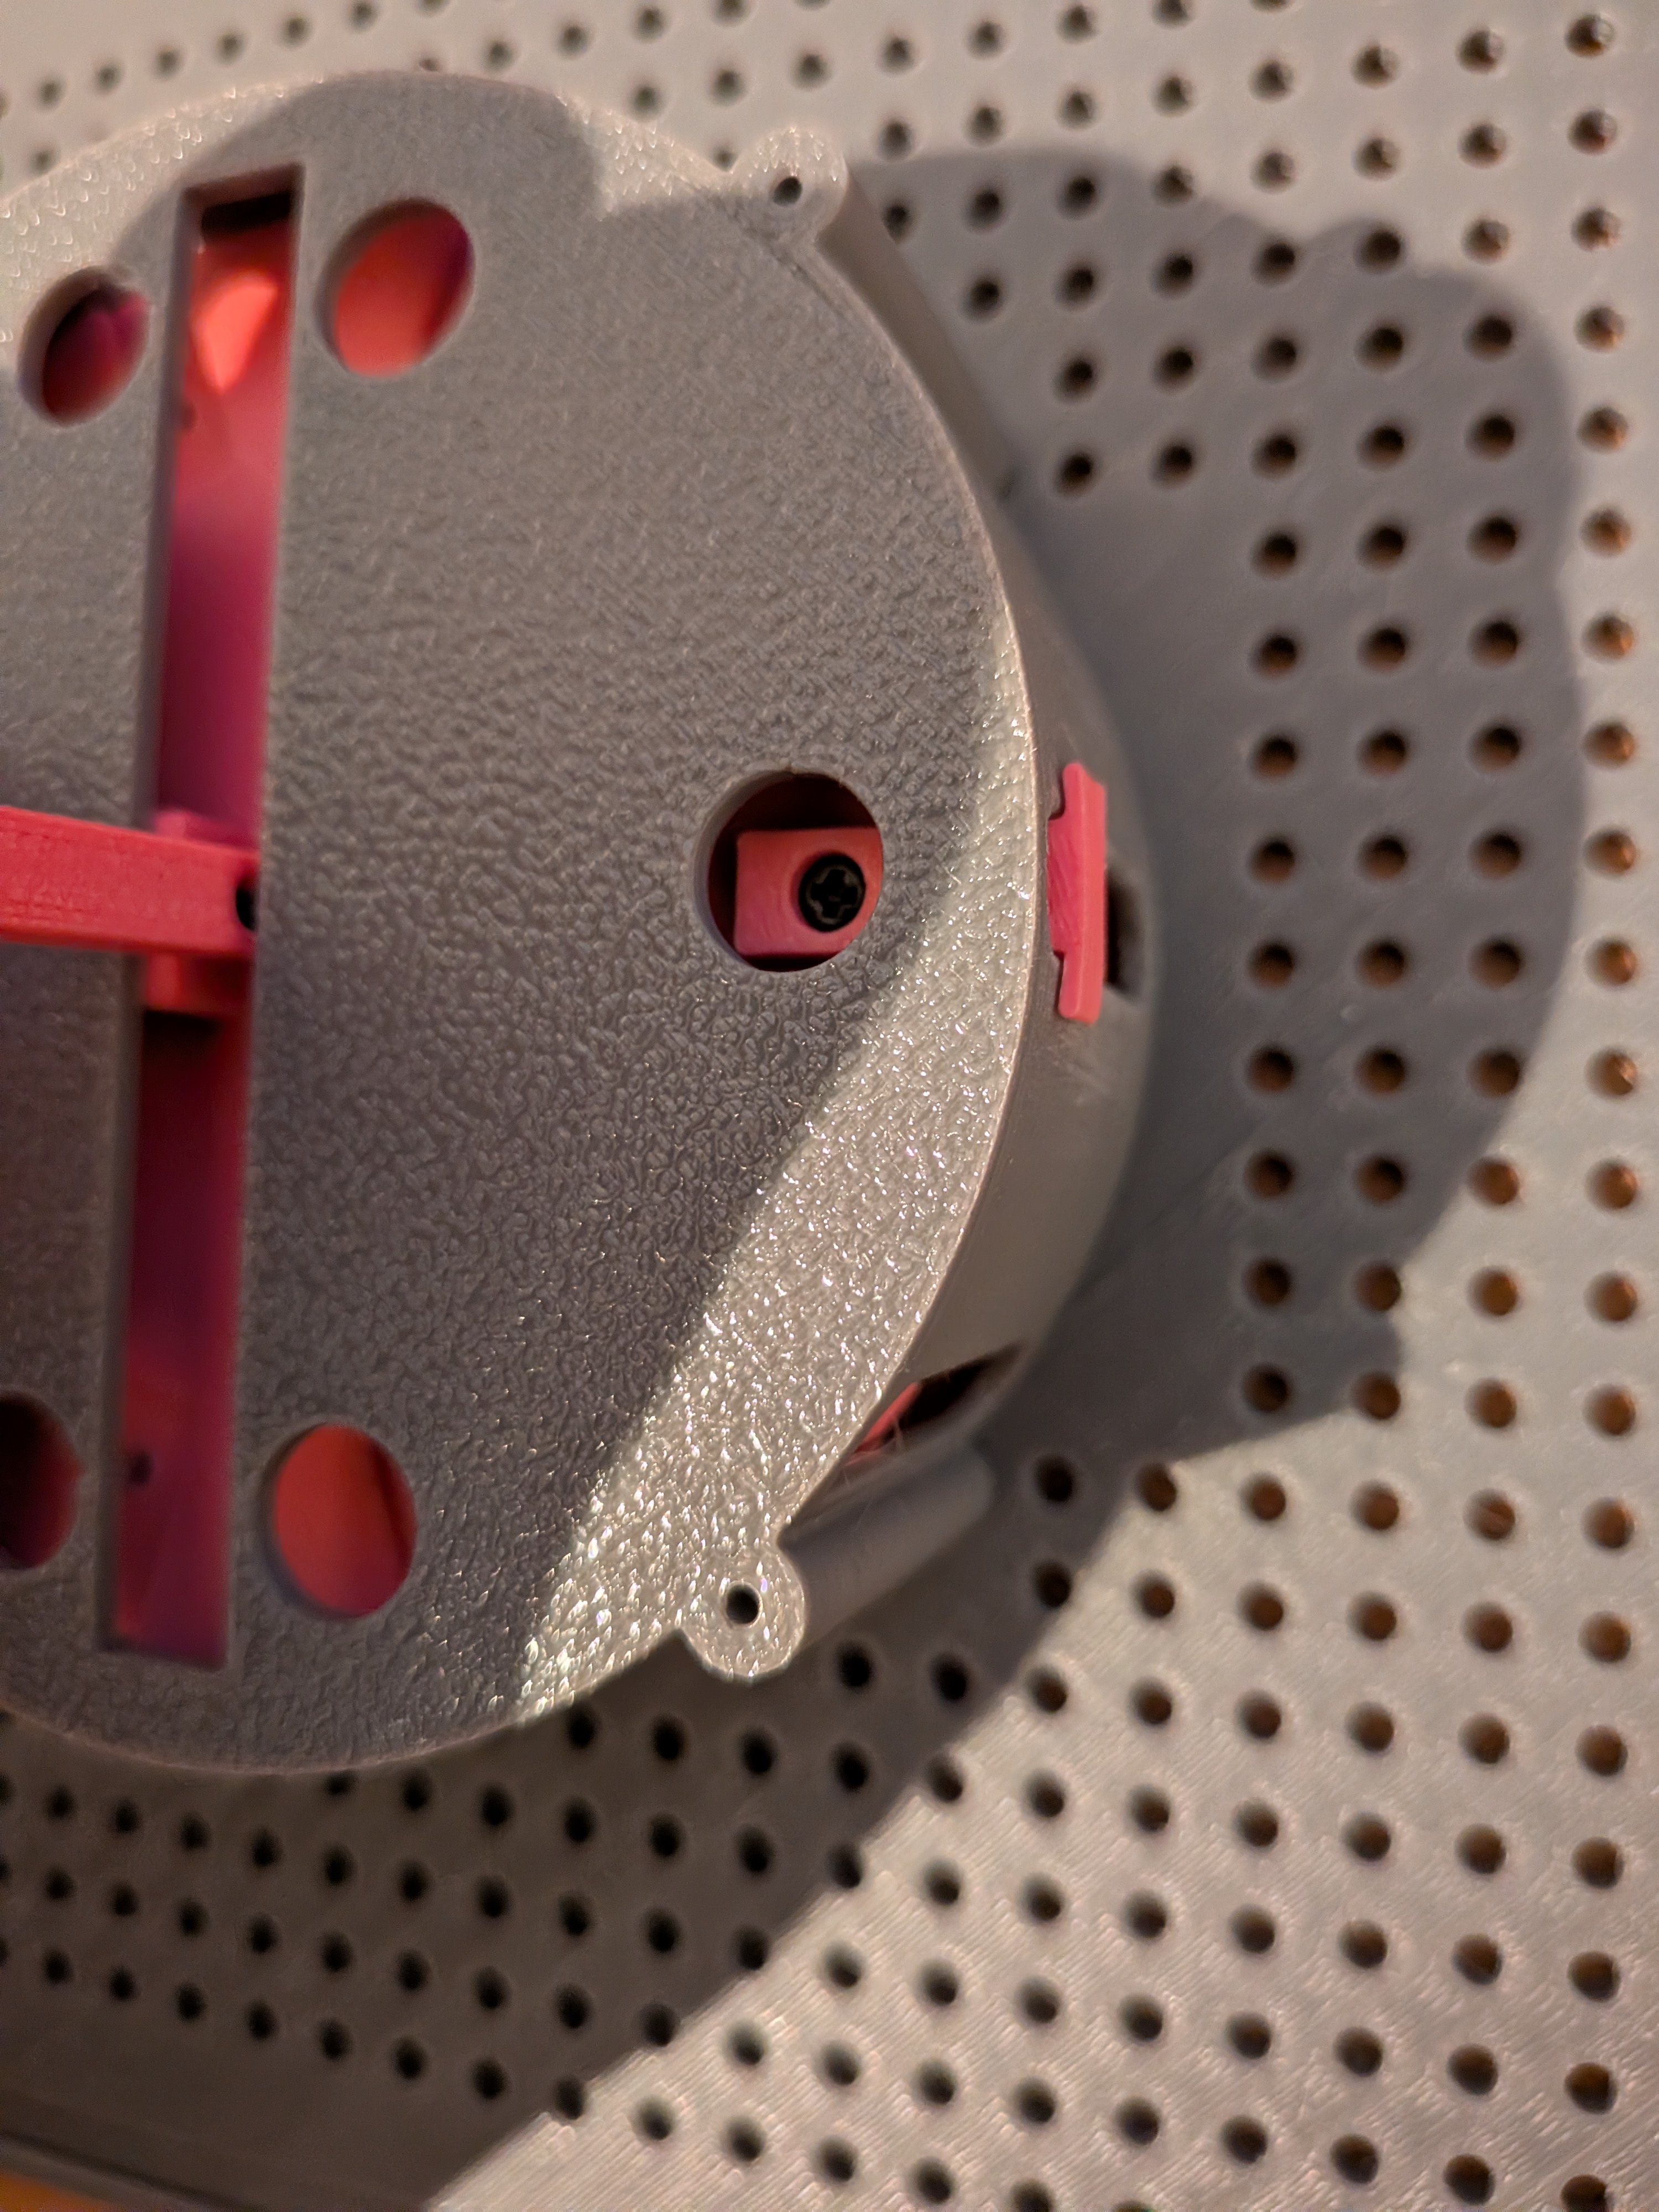
\includegraphics[scale=0.05]{montage_gereon/basis_konstrukt/PXL_20260909_073721737.jpg}

Dieser Vorgang wird für alle 5 Führungsachsen wiederholt:

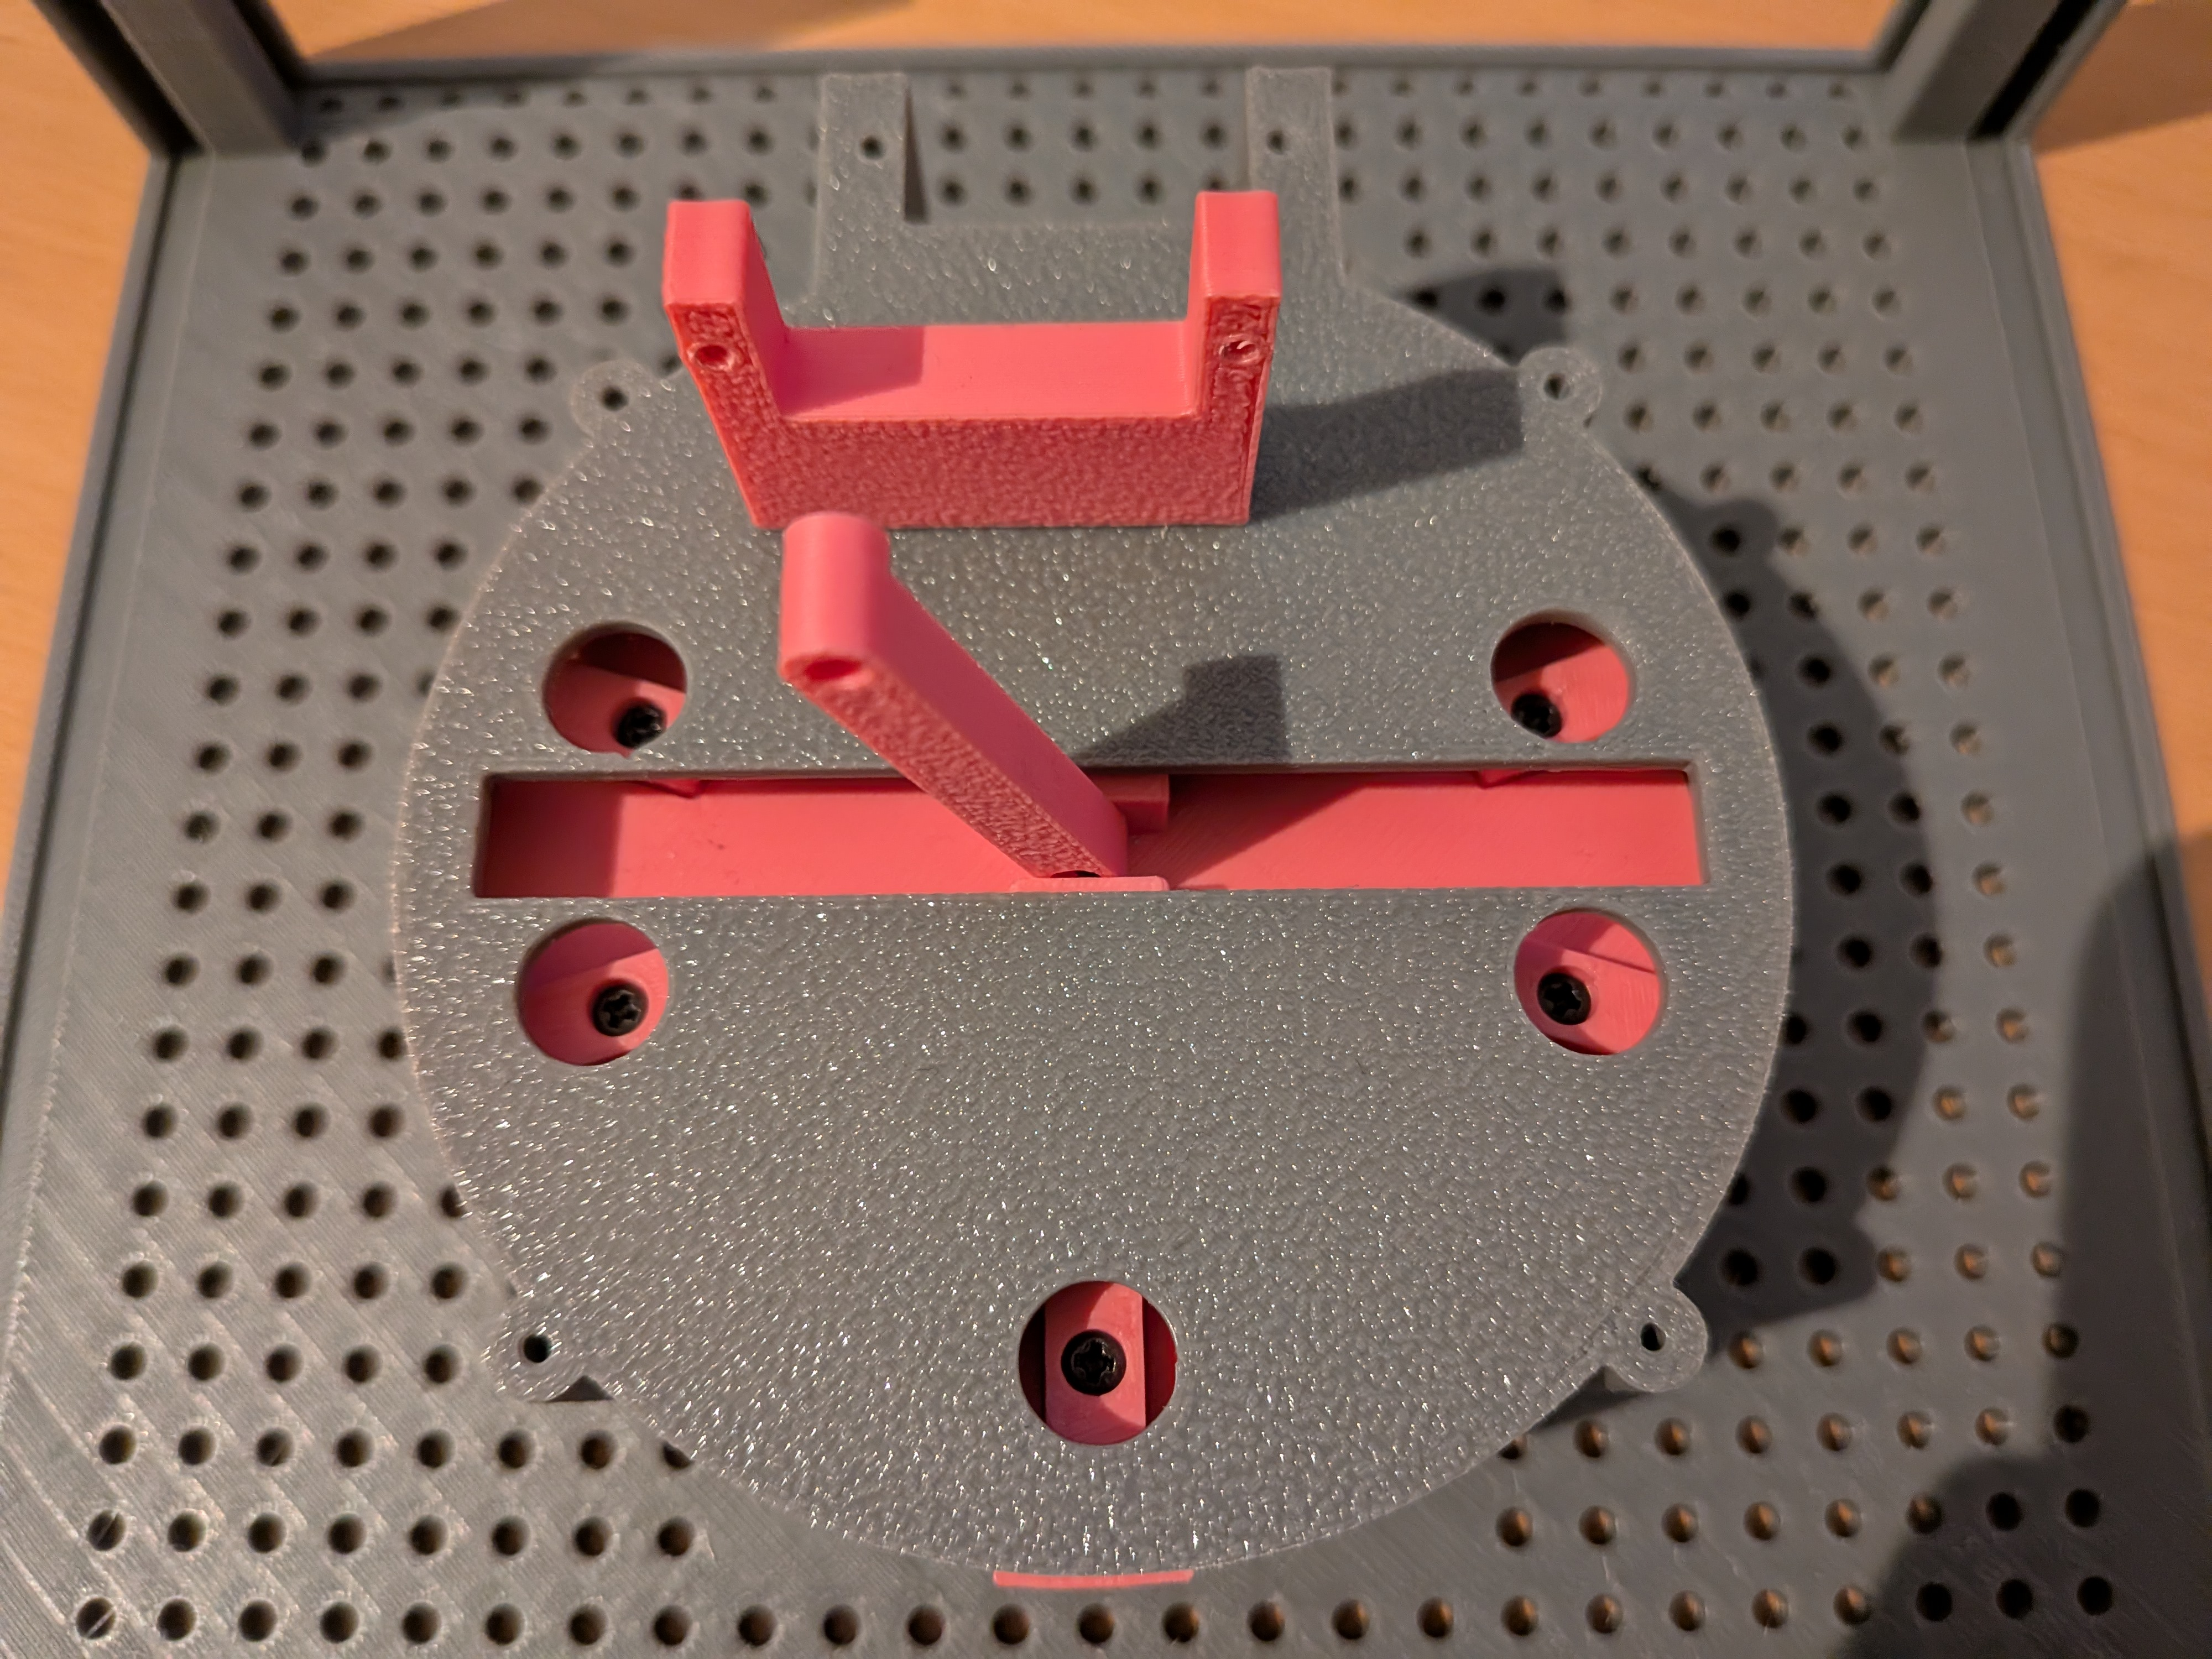
\includegraphics[scale=0.05]{montage_gereon/basis_konstrukt/PXL_20260909_074029247.jpg}


\begin{warnbox}
Wenn in den Öffnungen für die Führungsachsen wie in der nachfolgenden Darstellung gezeigt noch Reste des 3D-Drucks sind müssen diese nun entfernt werden, andernfalls ist die Bewegung des Coasterträgers nicht flüßig. 

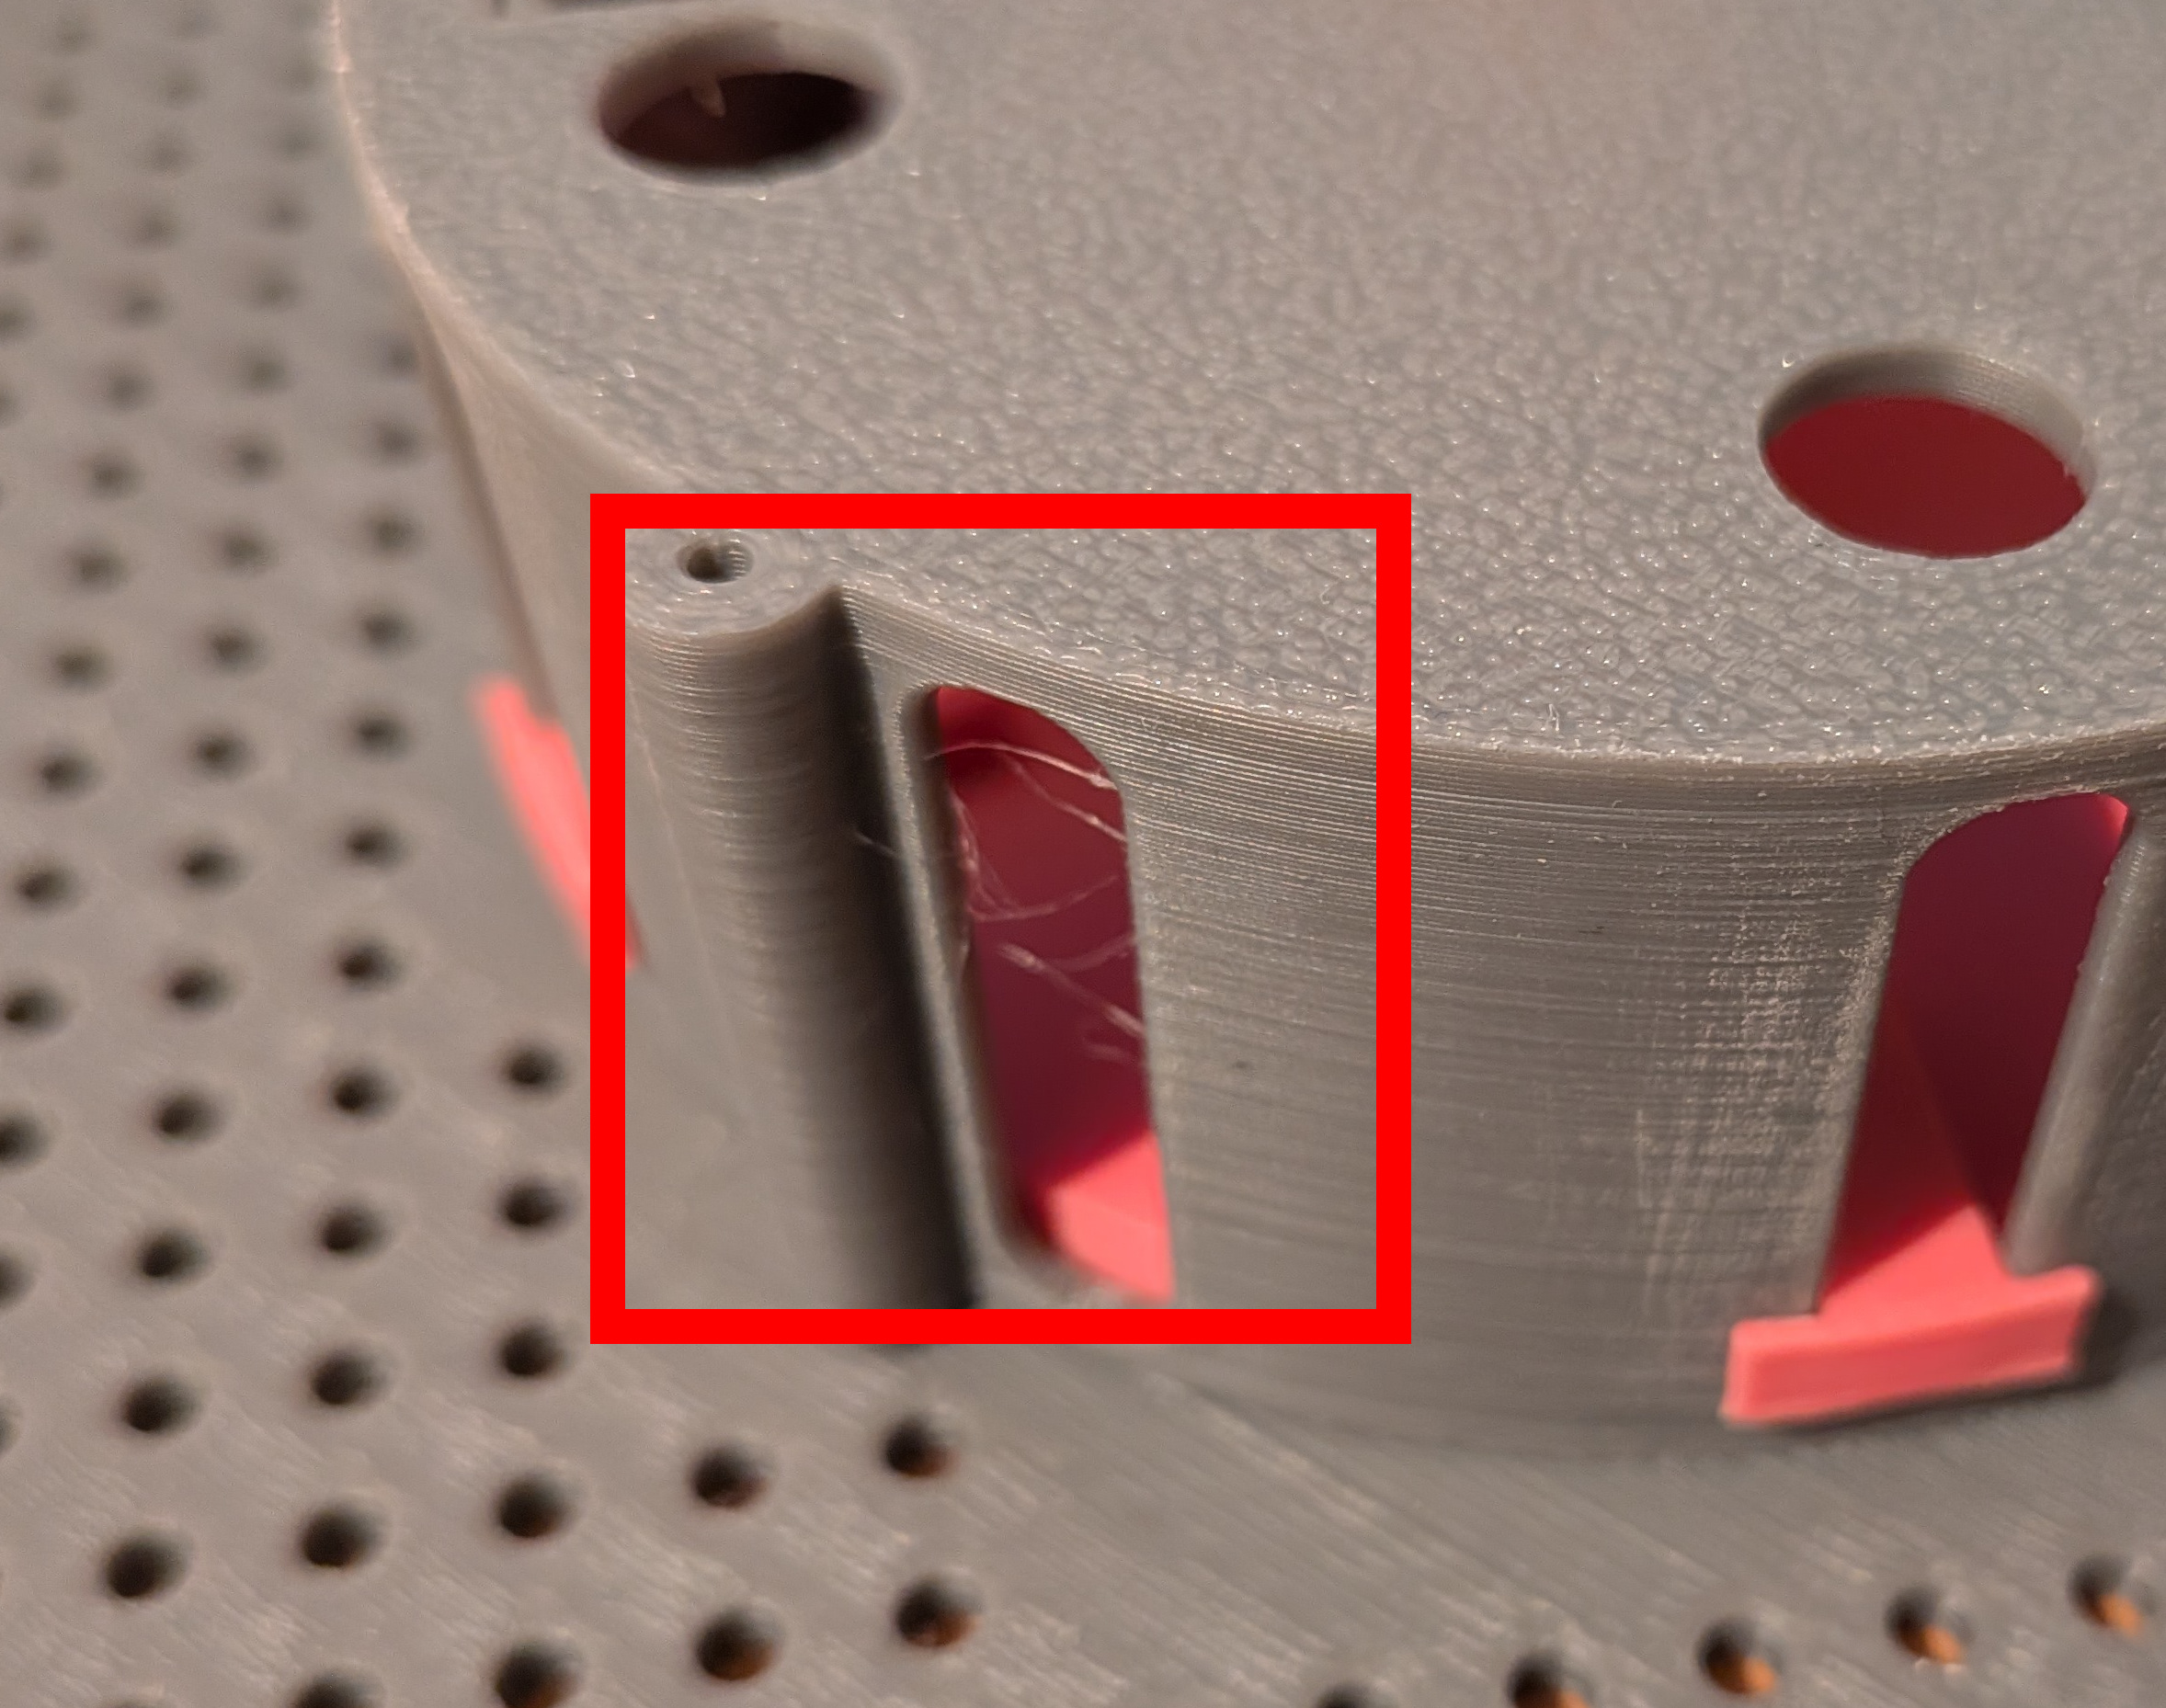
\includegraphics[scale=0.10]{montage_gereon/basis_konstrukt/PXL_20260909_074048115.jpg}
\end{warnbox}


\subsection{Coasteraufnahme Servos montieren}

Nun werden die Servos auf der Coasteraufnahme montiert. Zunächst wird der obere Servo eingesetzt und beidseitig verschraubt.

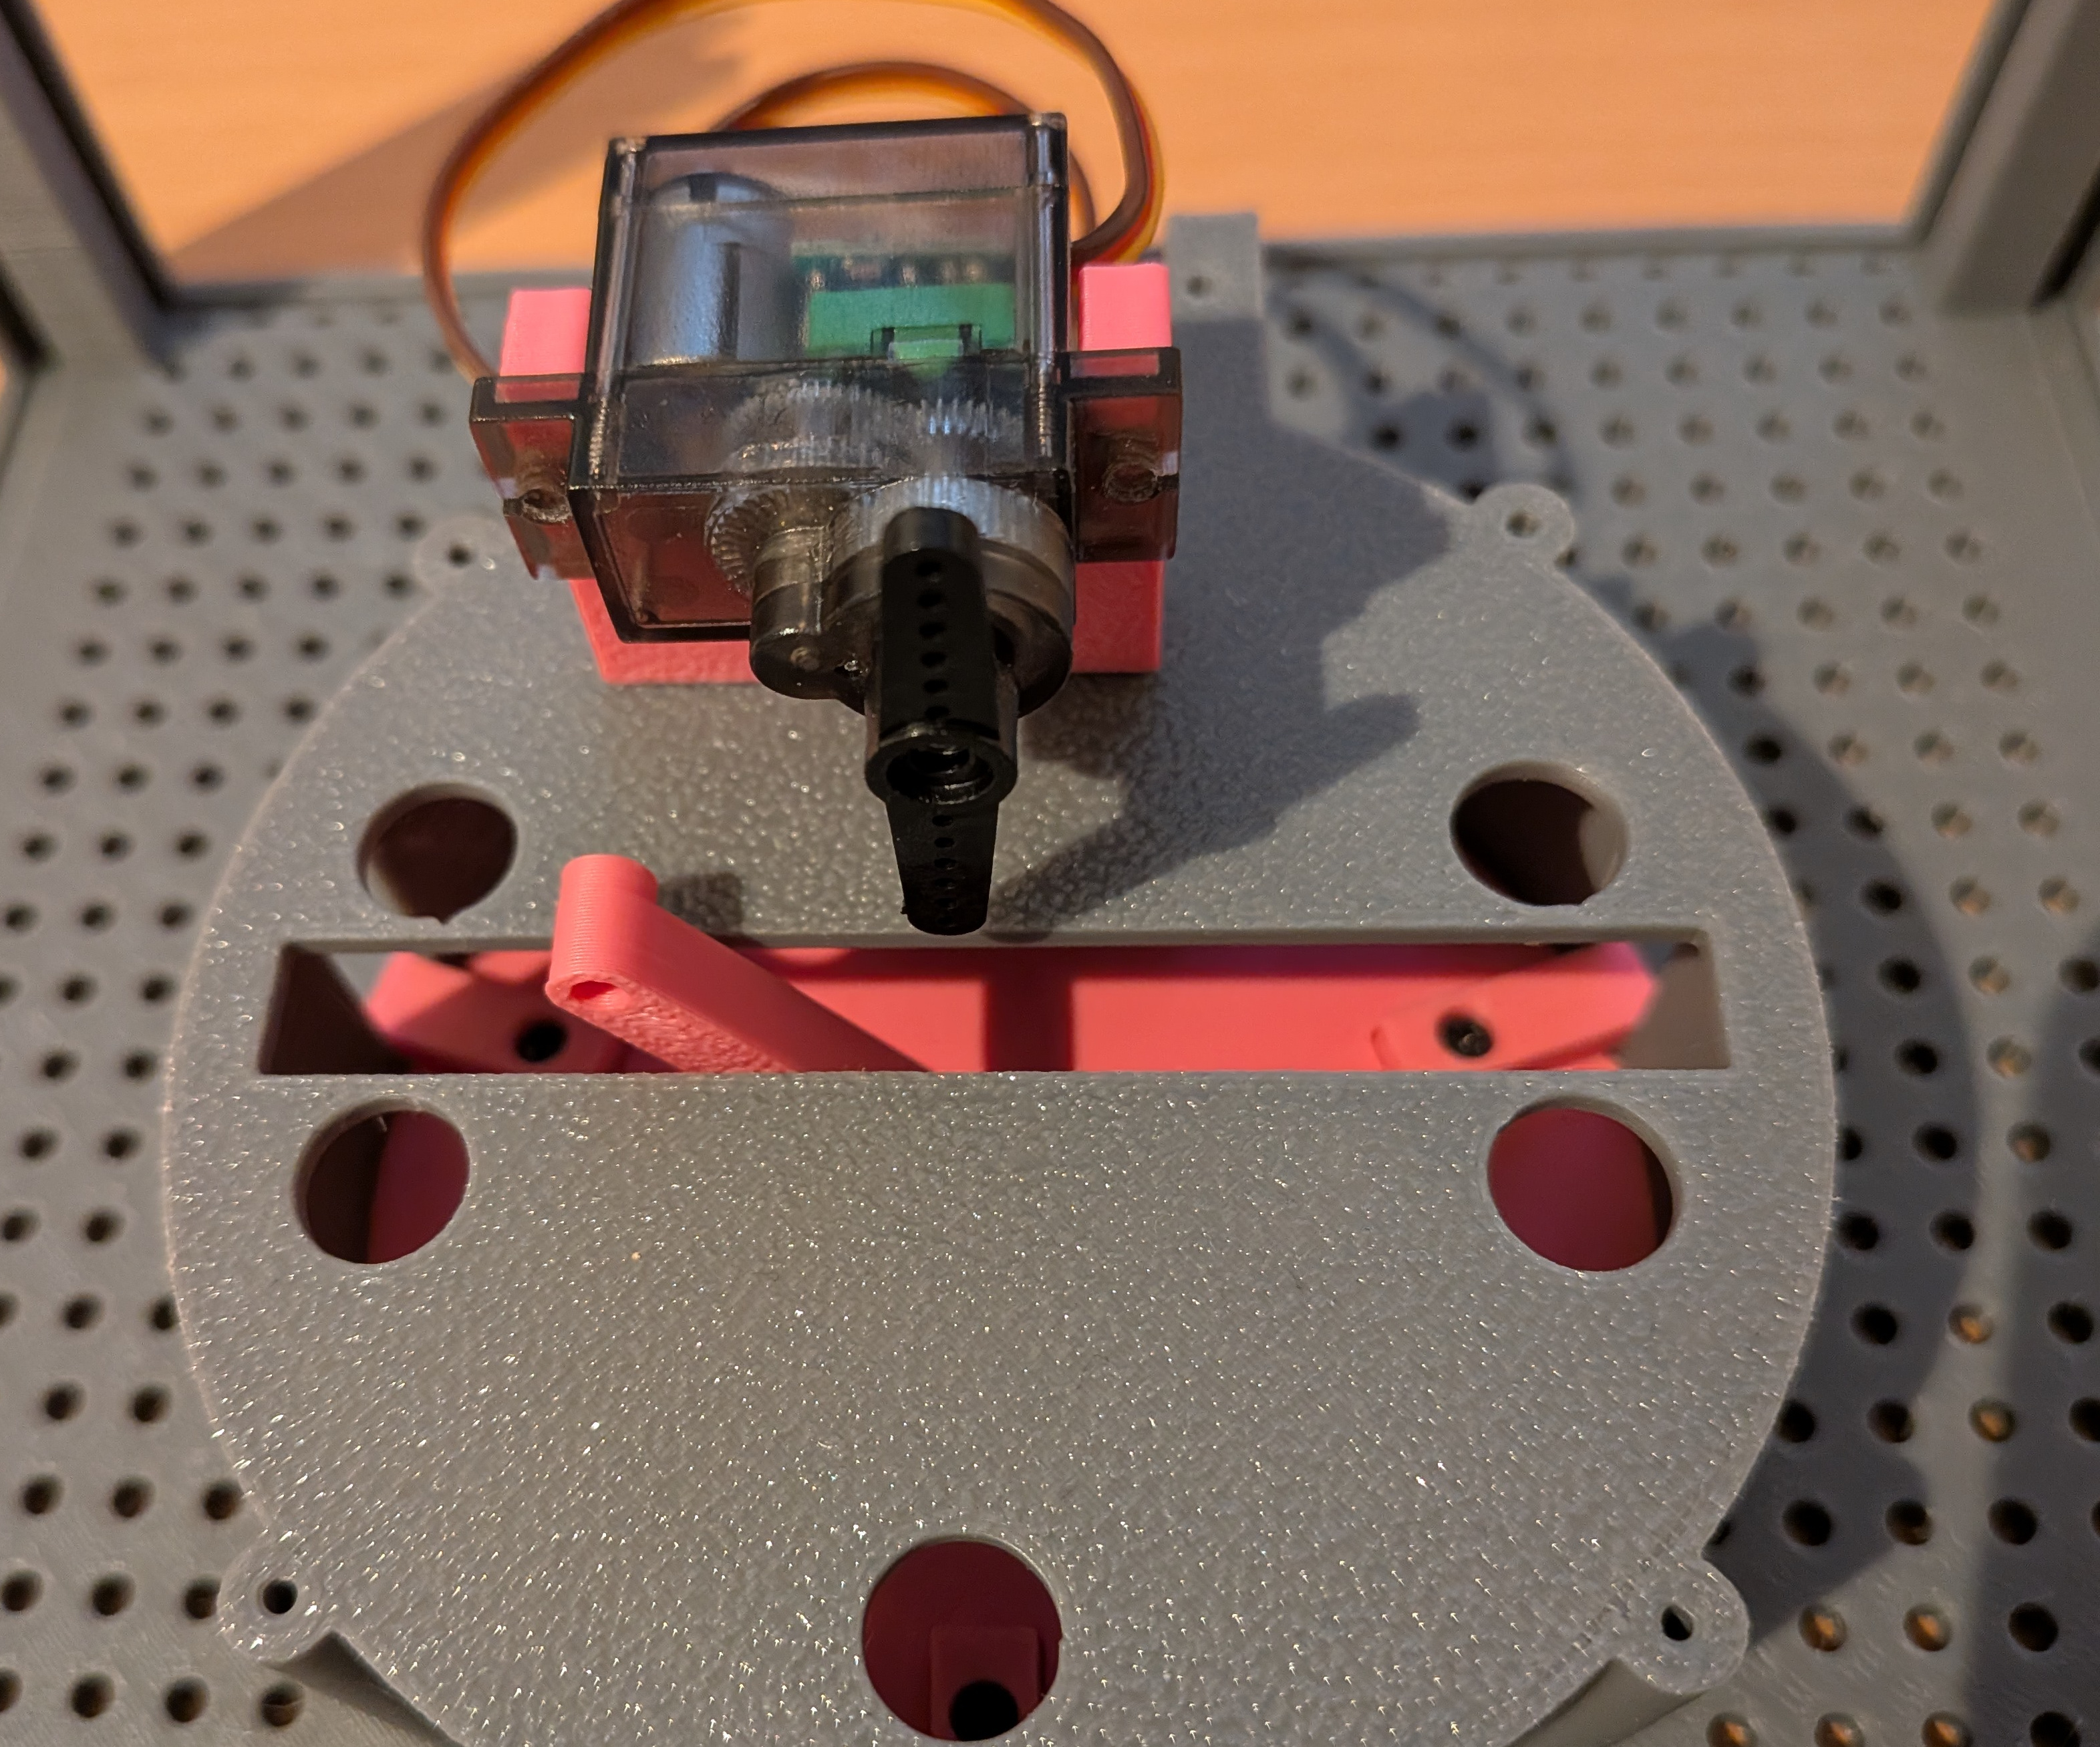
\includegraphics[scale=0.07]{montage_gereon/servo_montage/PXL_20260909_074828749.jpg}

An diesem wird nun der Zugträger des Coasteraufnahmemechanimus befestigt:

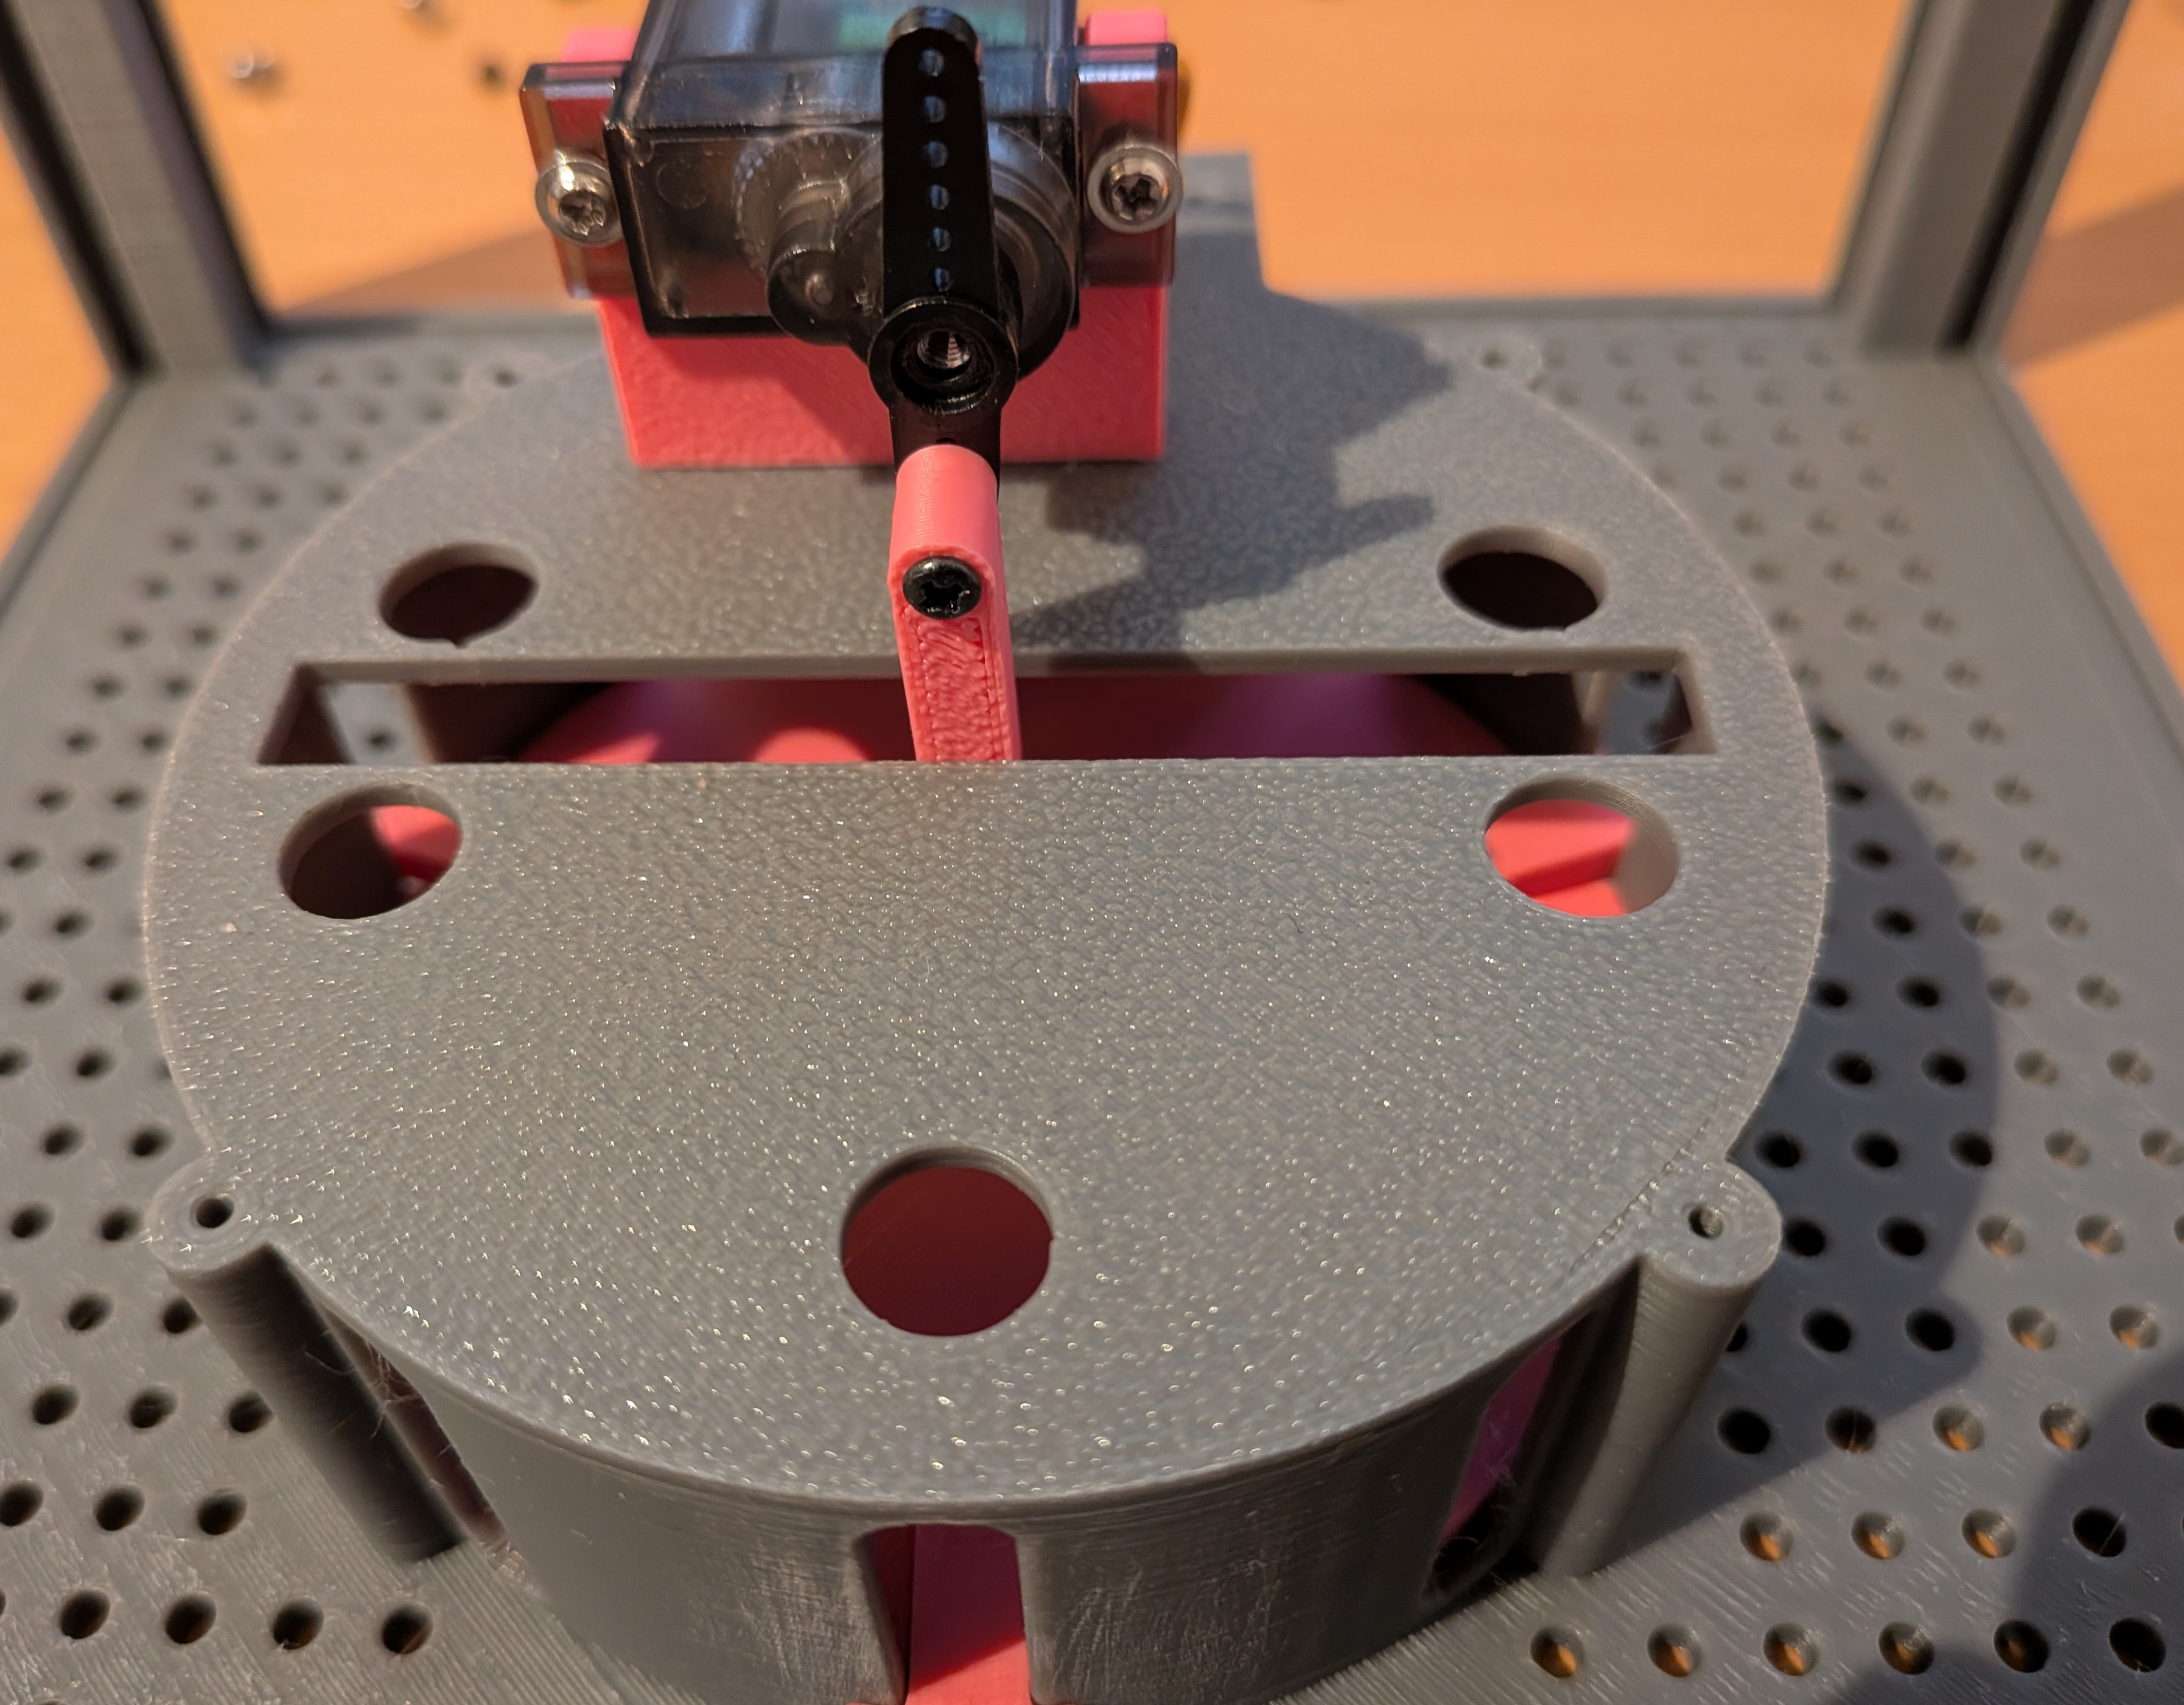
\includegraphics[scale=0.07]{montage_gereon/servo_montage/PXL_20260909_075115487.jpg}


Nun muss der zweite Servo in der seitlichen Halteschiene eingesetzt werden. Abhängig vom Servomodell und der zuweilen unterschiedlichen Kabelausführung aus dem Gehäuse kann dies etwas eng werden, ist aber auch in diesen Fällen möglich. Der Servo wird hier ebenfalls fixiert. 


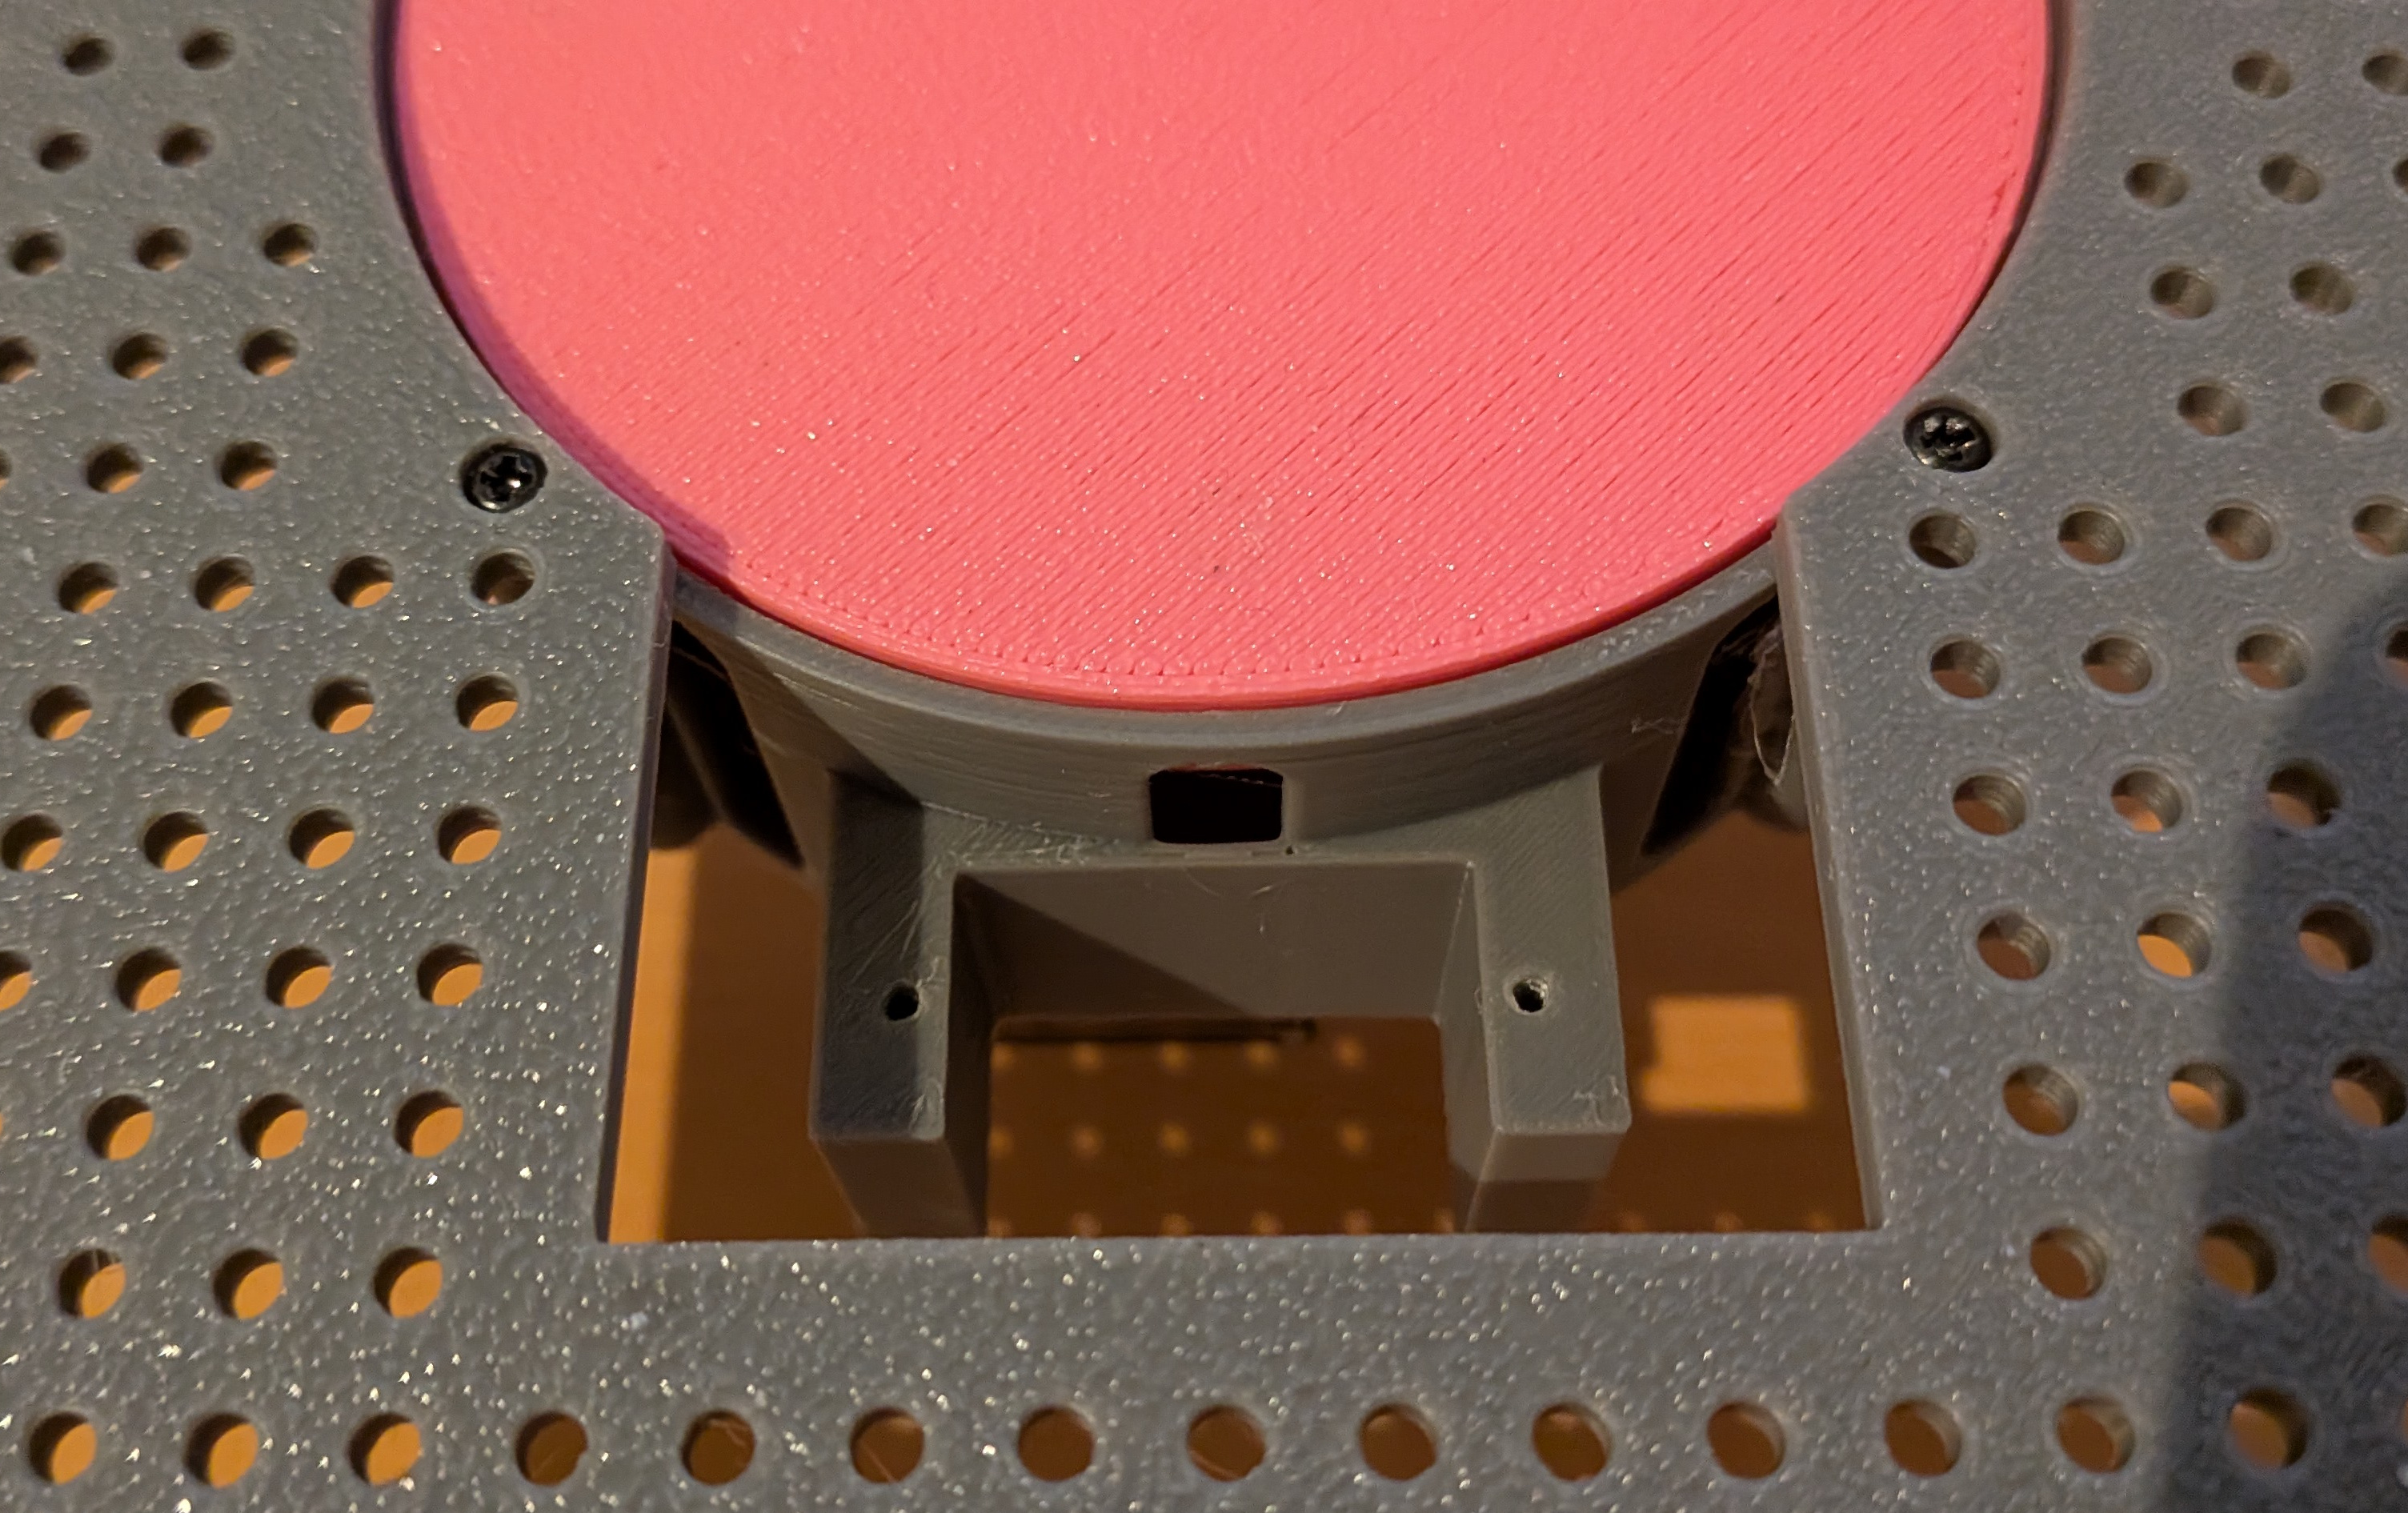
\includegraphics[scale=0.07]{montage_gereon/servo_montage/PXL_20260909_075226995.jpg}
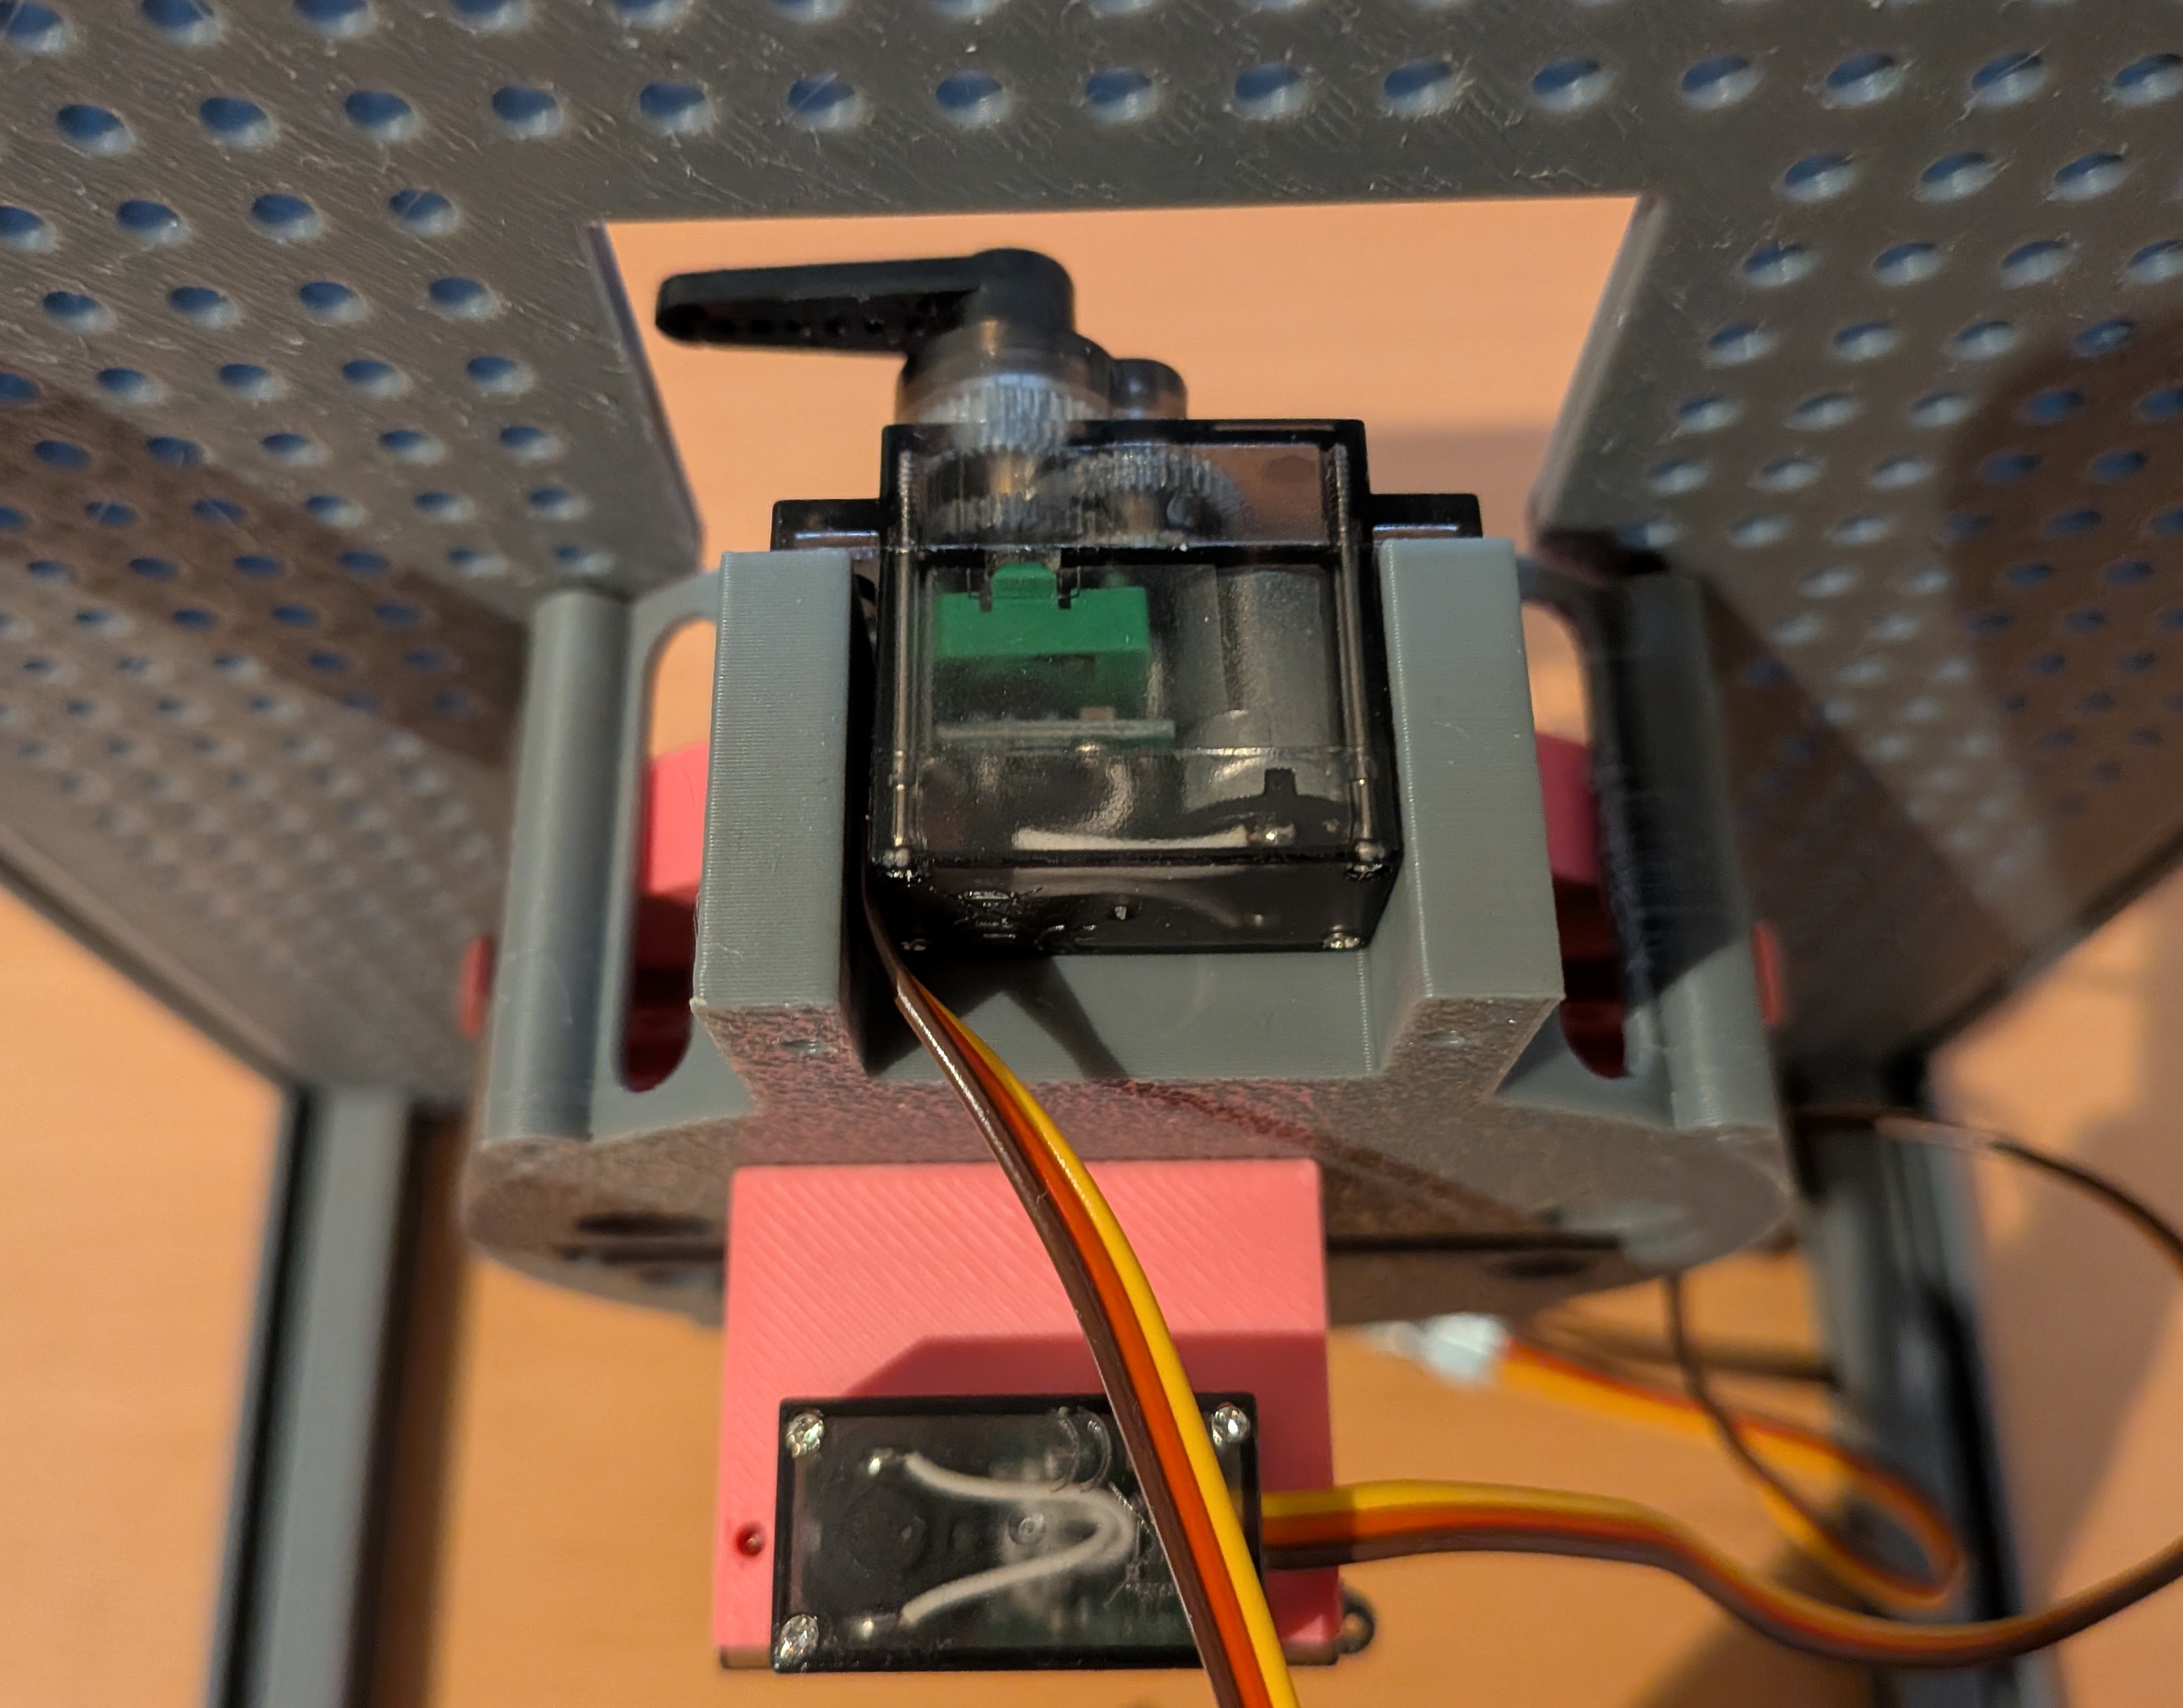
\includegraphics[scale=0.06]{montage_gereon/servo_montage/PXL_20260909_080007064.jpg}

Anschließend muss der Arm zum Ausschunb der Coaster noch aufgesetzt und verschraubt werden:

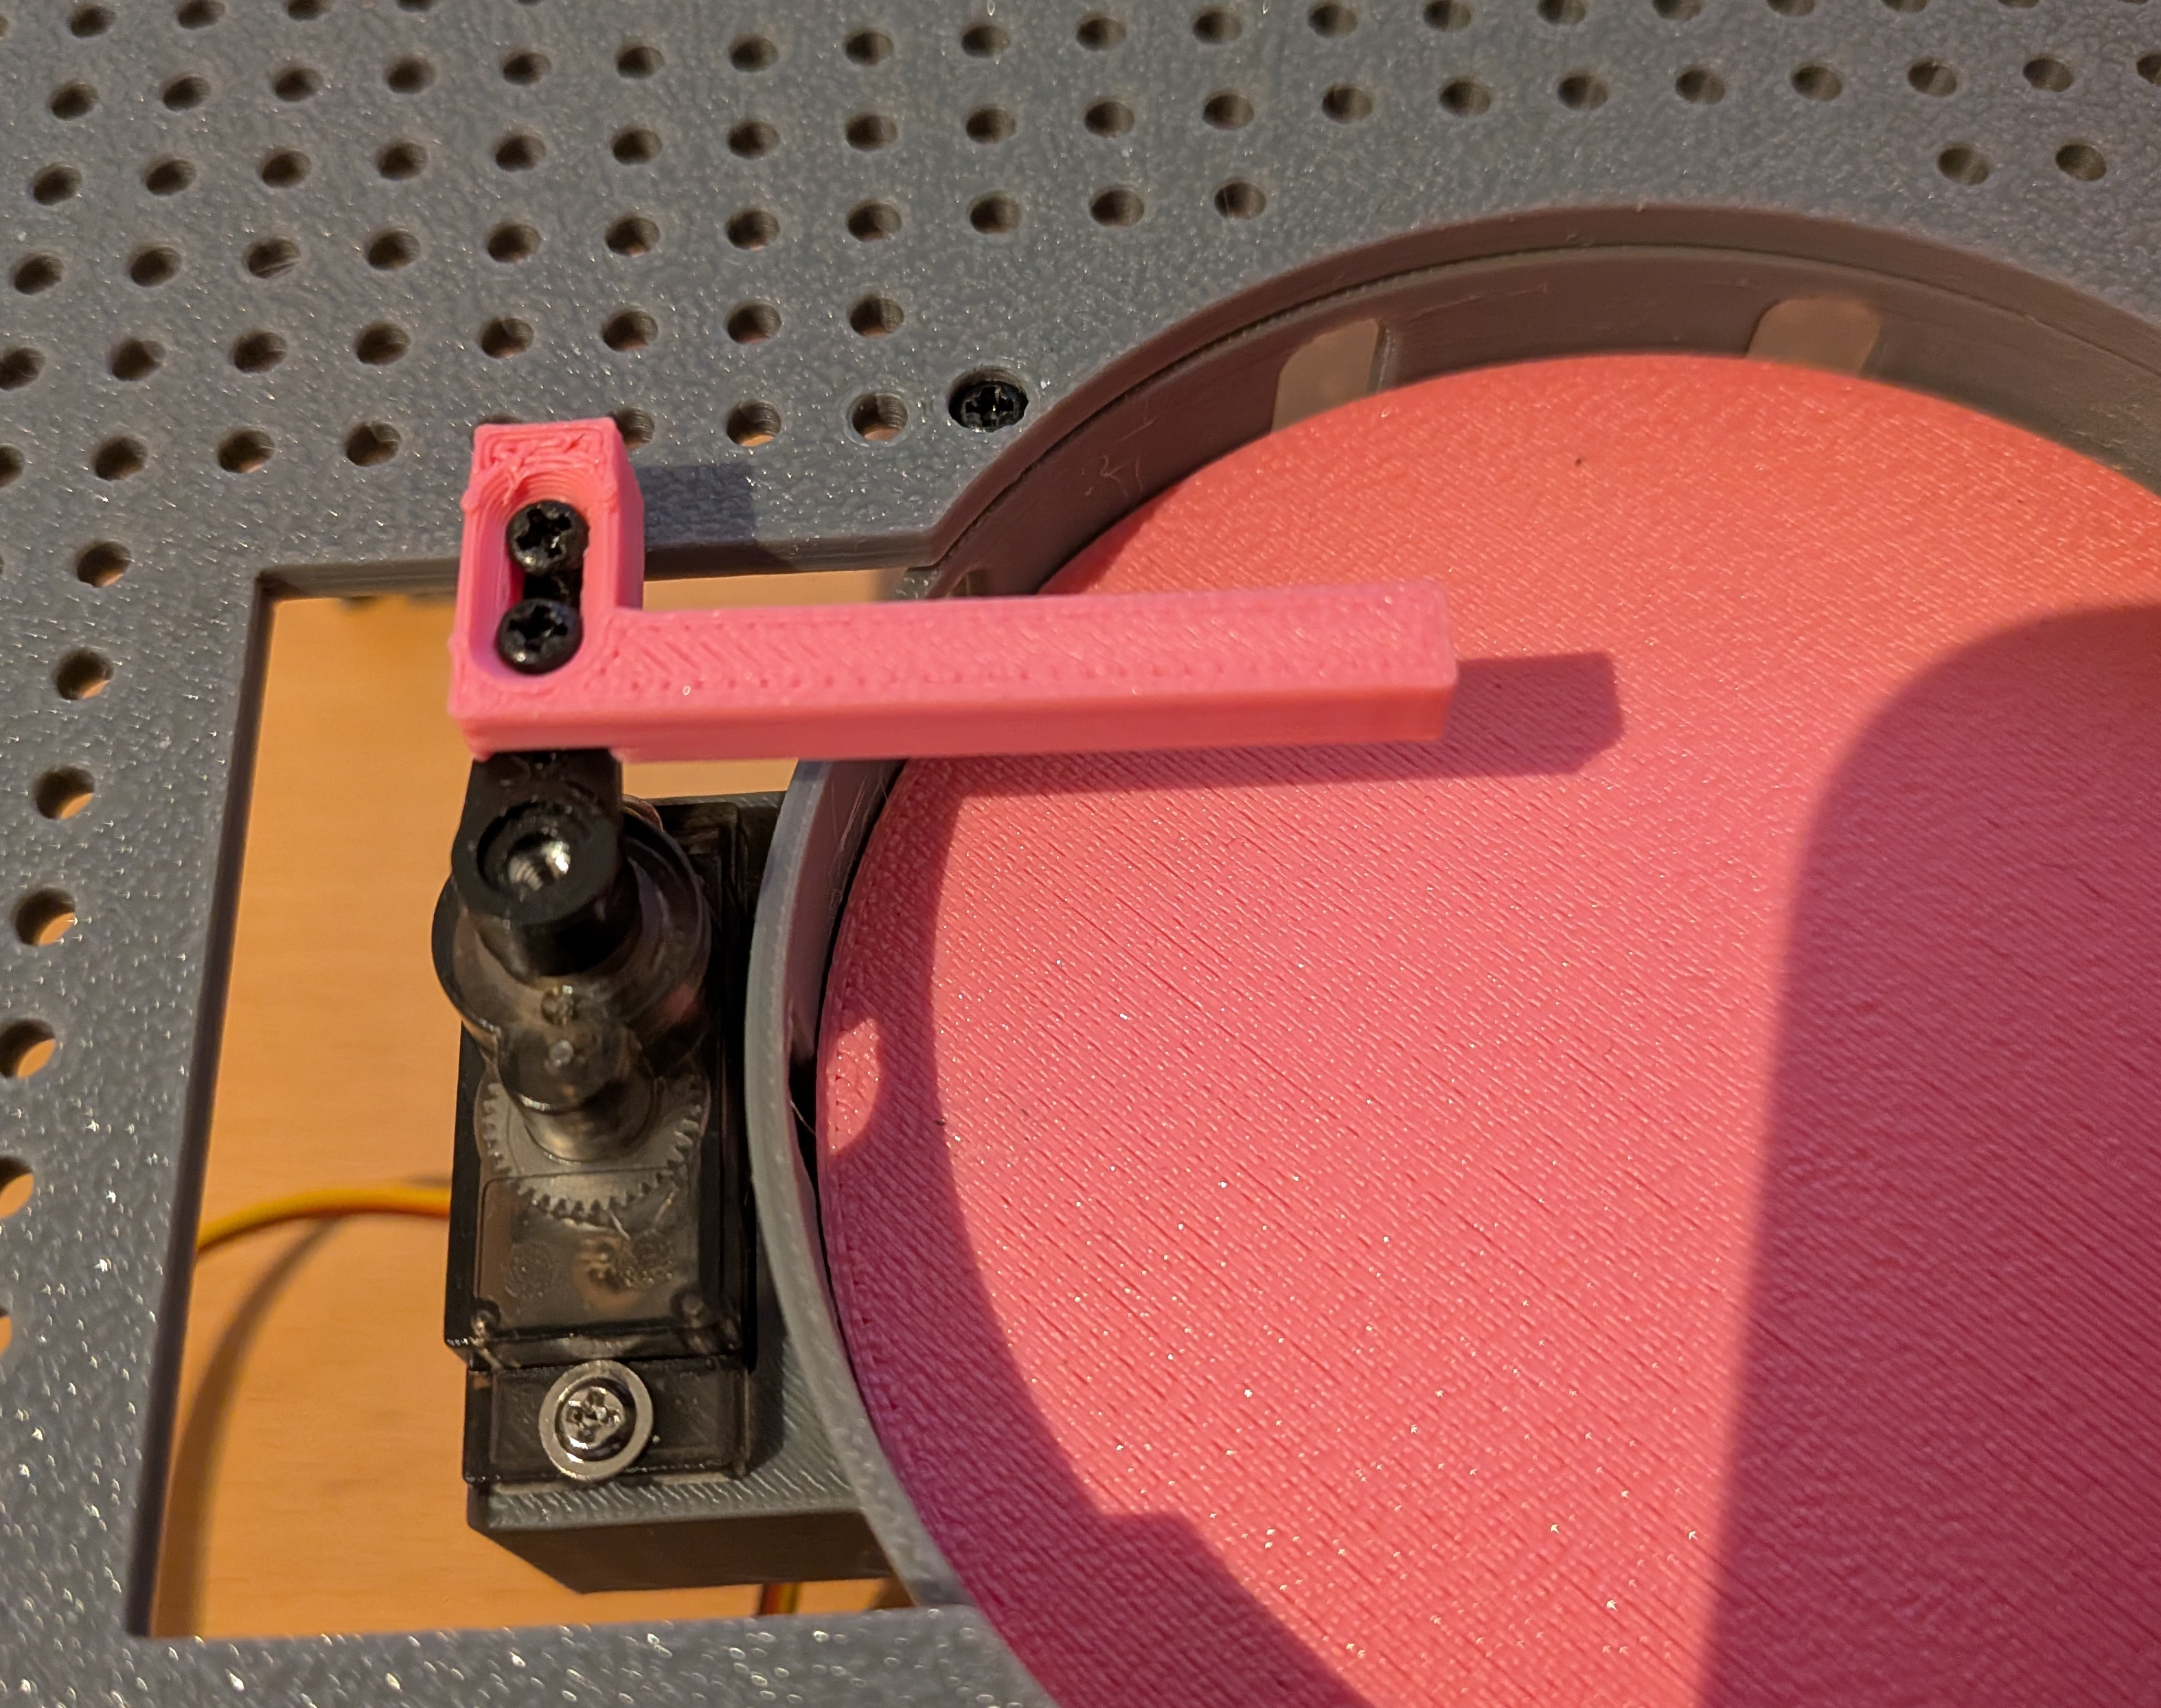
\includegraphics[scale=0.09]{montage_gereon/servo_montage/PXL_20260909_080331090.jpg}



\subsection{Sensorik montieren}

Nun erfolgt die Montage der Sensorik Module

\subsubsection{Tischkantenerkennung}

Zur Montage der 4 Tischkantensensoren bedarf es jeweils einer Infrarot Abstandsmessungsplatine und für die Gehäuse einer Grundplatte und der Abdeckung:

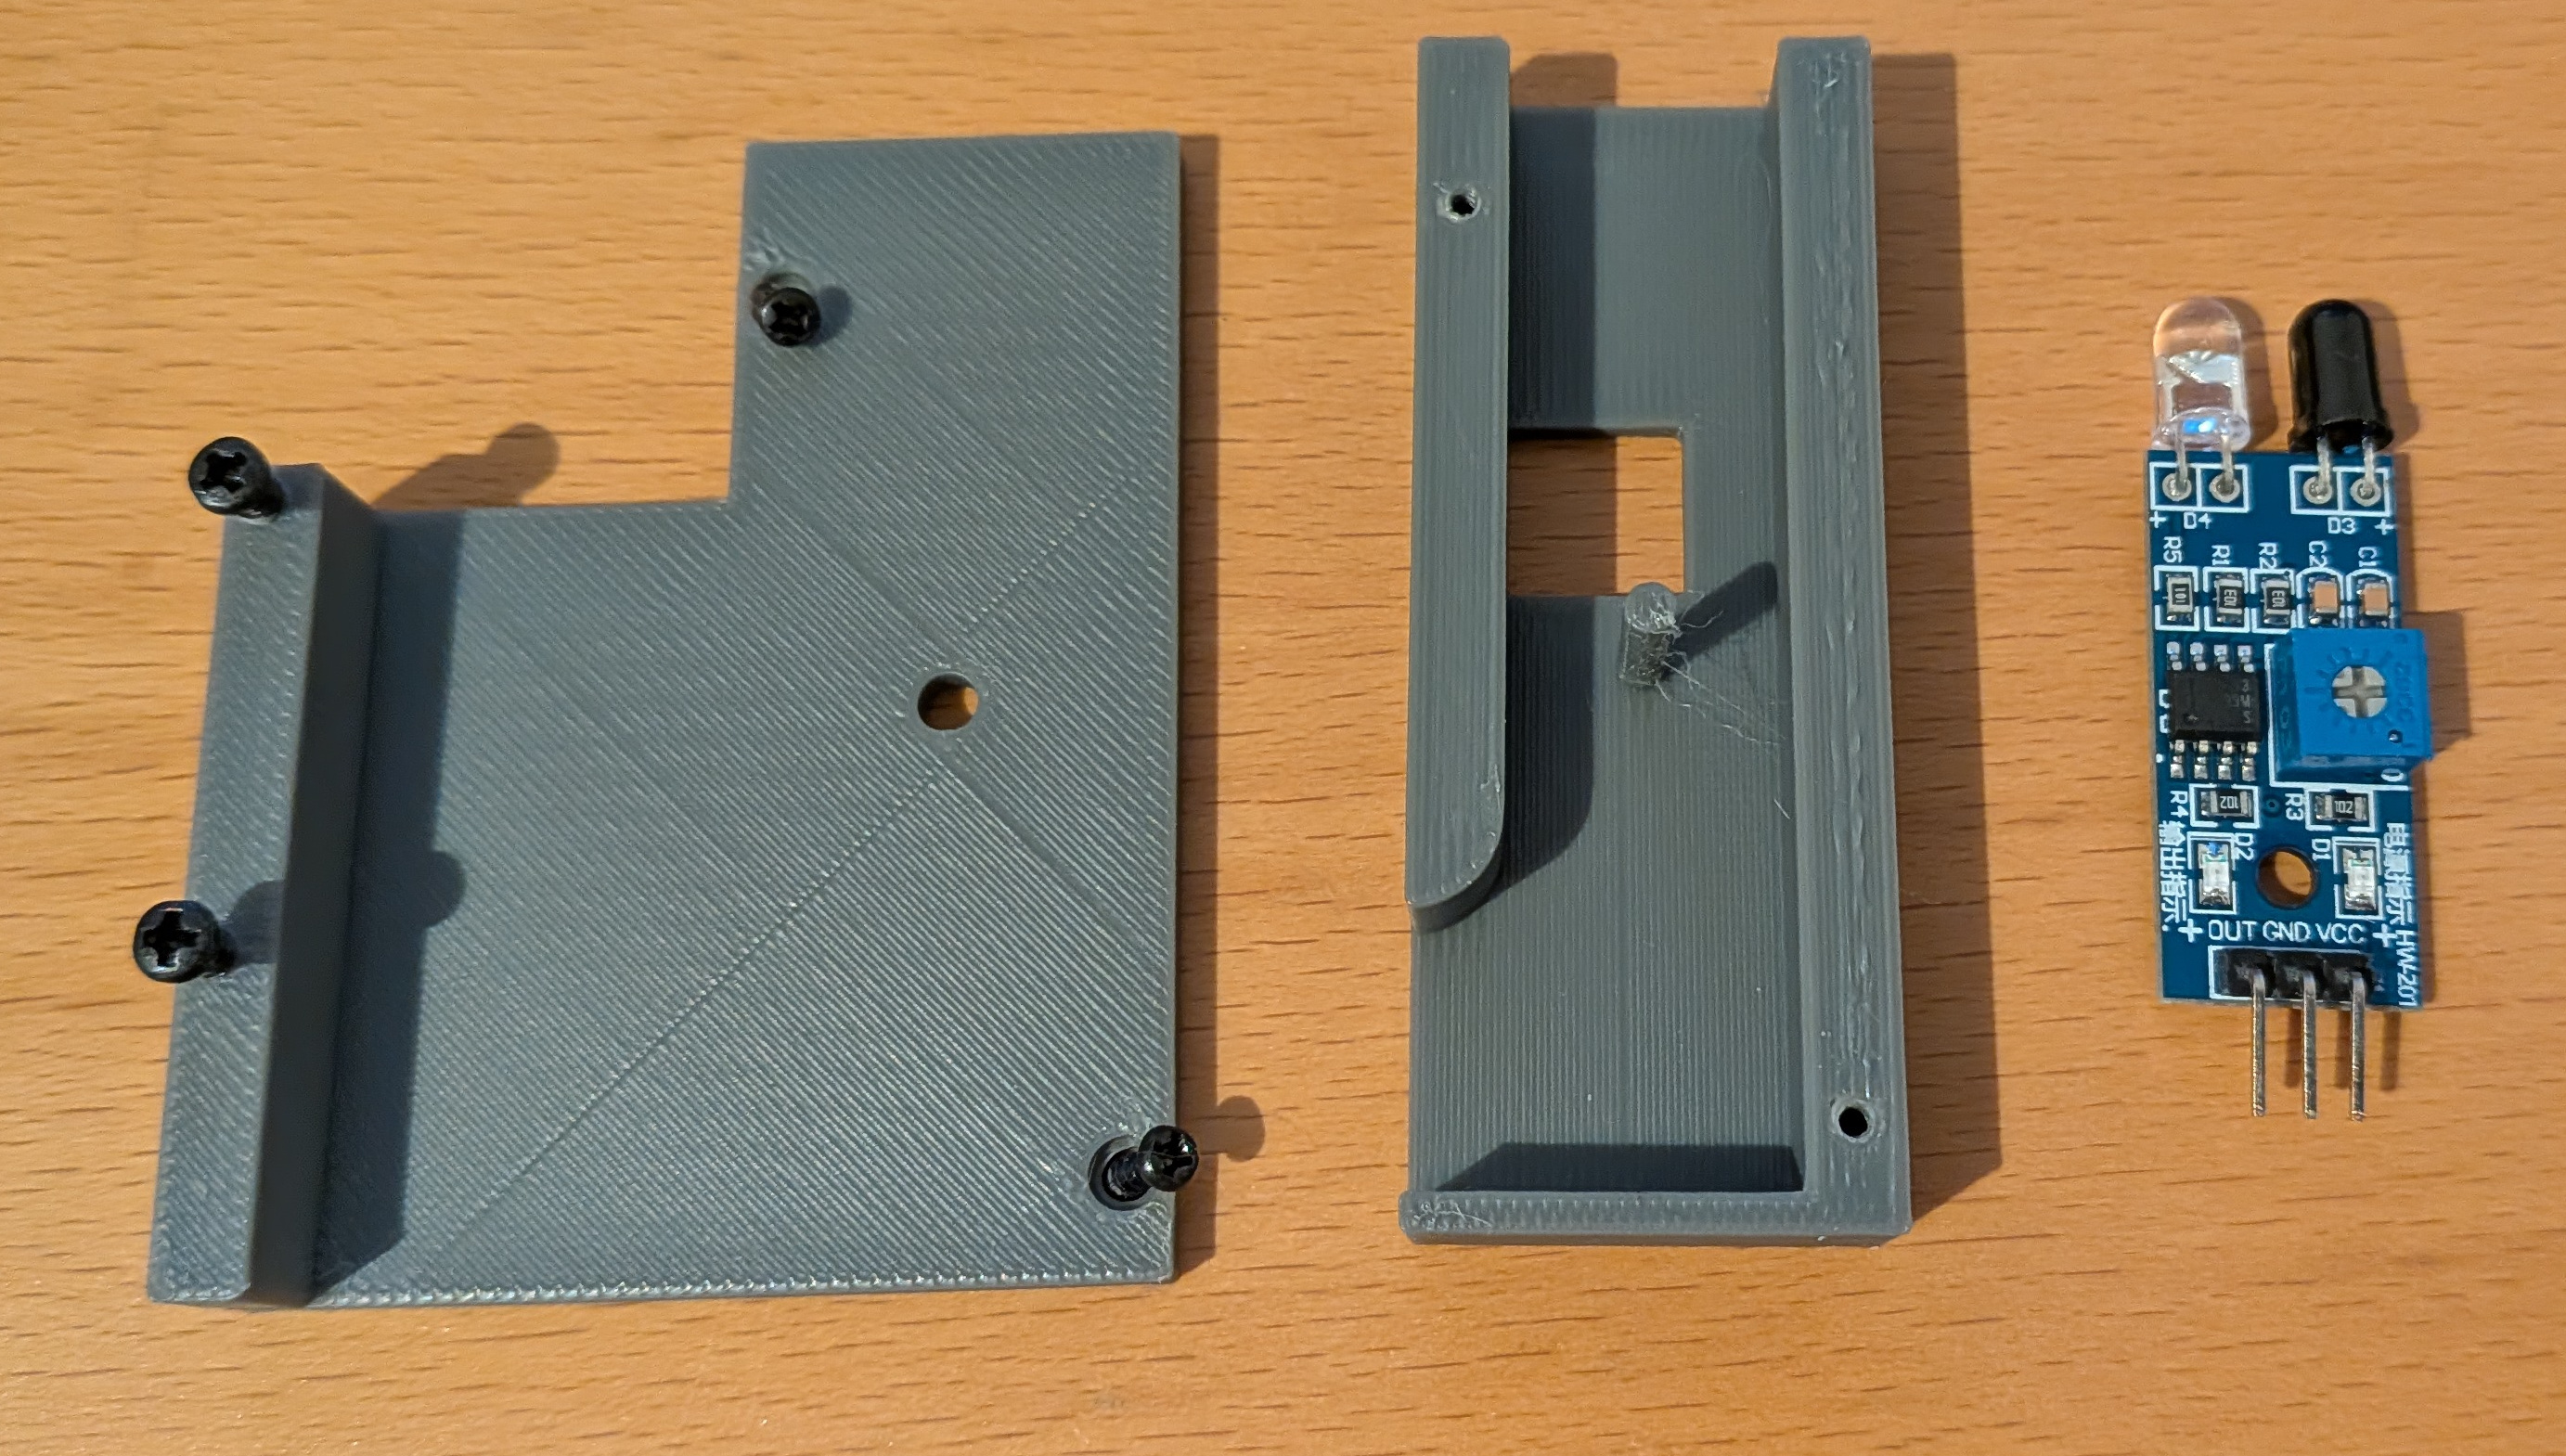
\includegraphics[scale=0.08]{montage_gereon/tischkantensensor/PXL_20260907_153310192.jpg}

Hier wird zunächst das dreiadrige Flachbandkabel mit den Steckverbindern montiert.

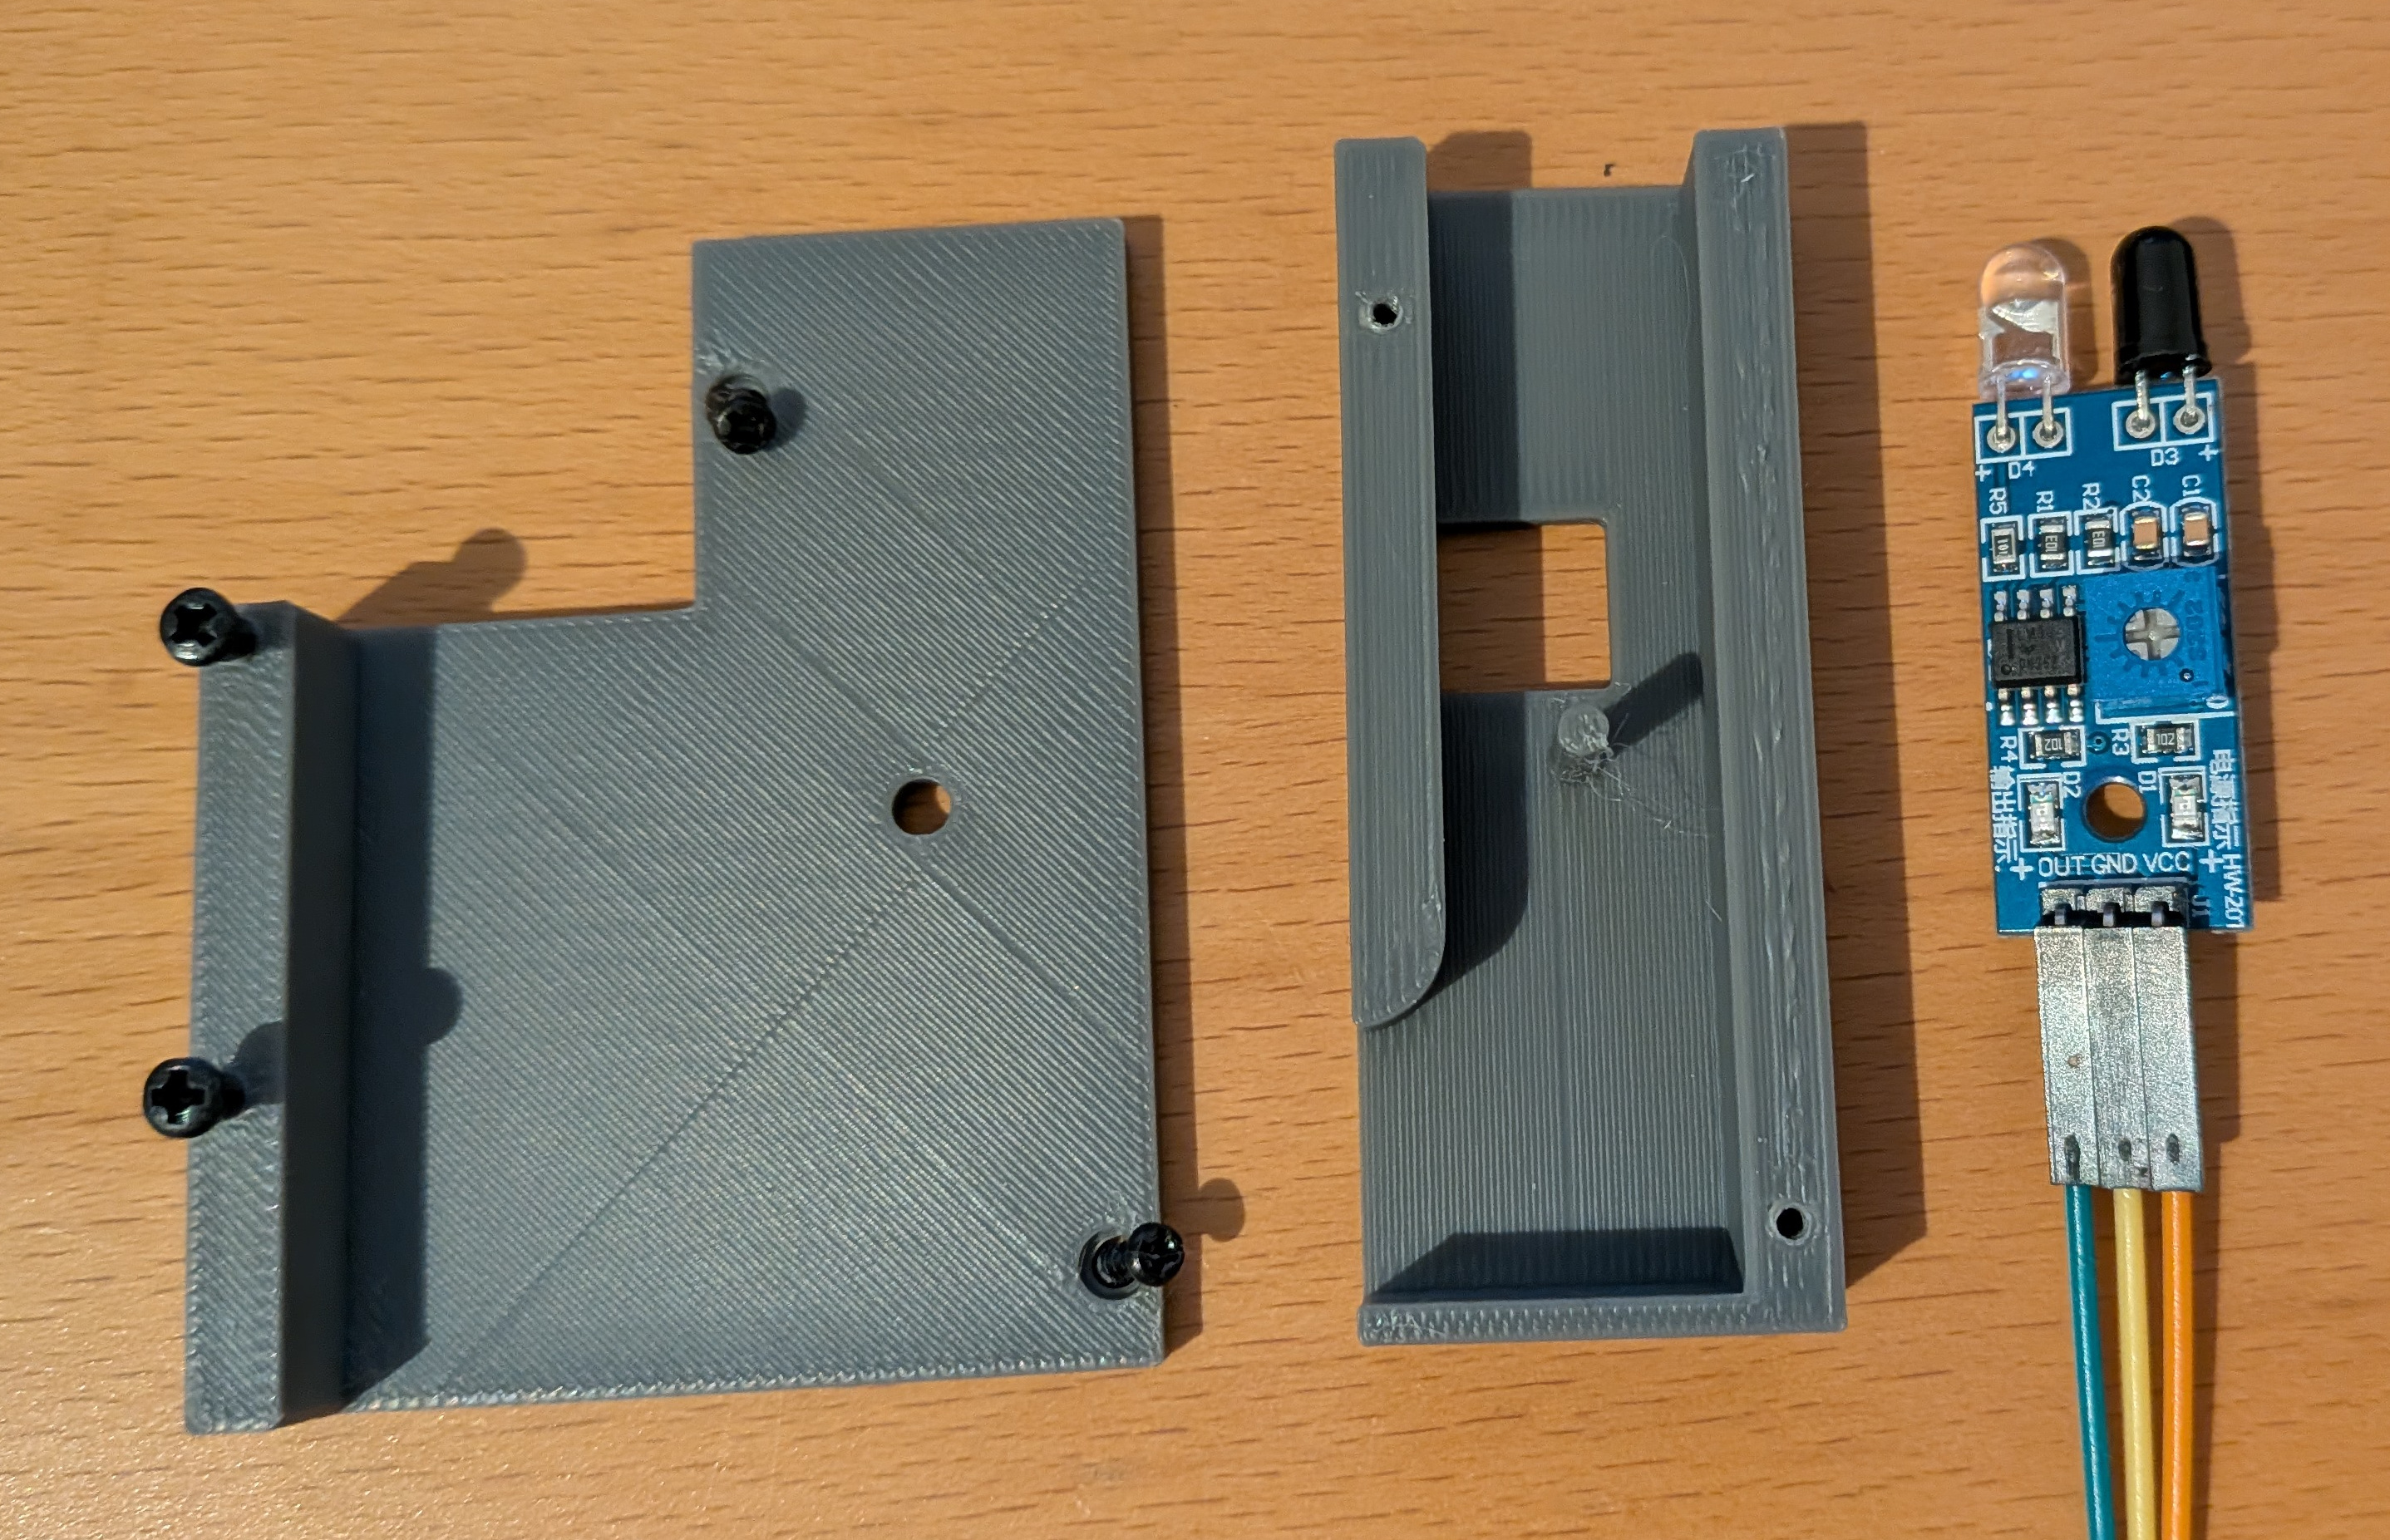
\includegraphics[scale=0.08]{montage_gereon/tischkantensensor/PXL_20260907_153358087.jpg}

Anschließend wird die Sensorplatine im Gehäuse platziert:

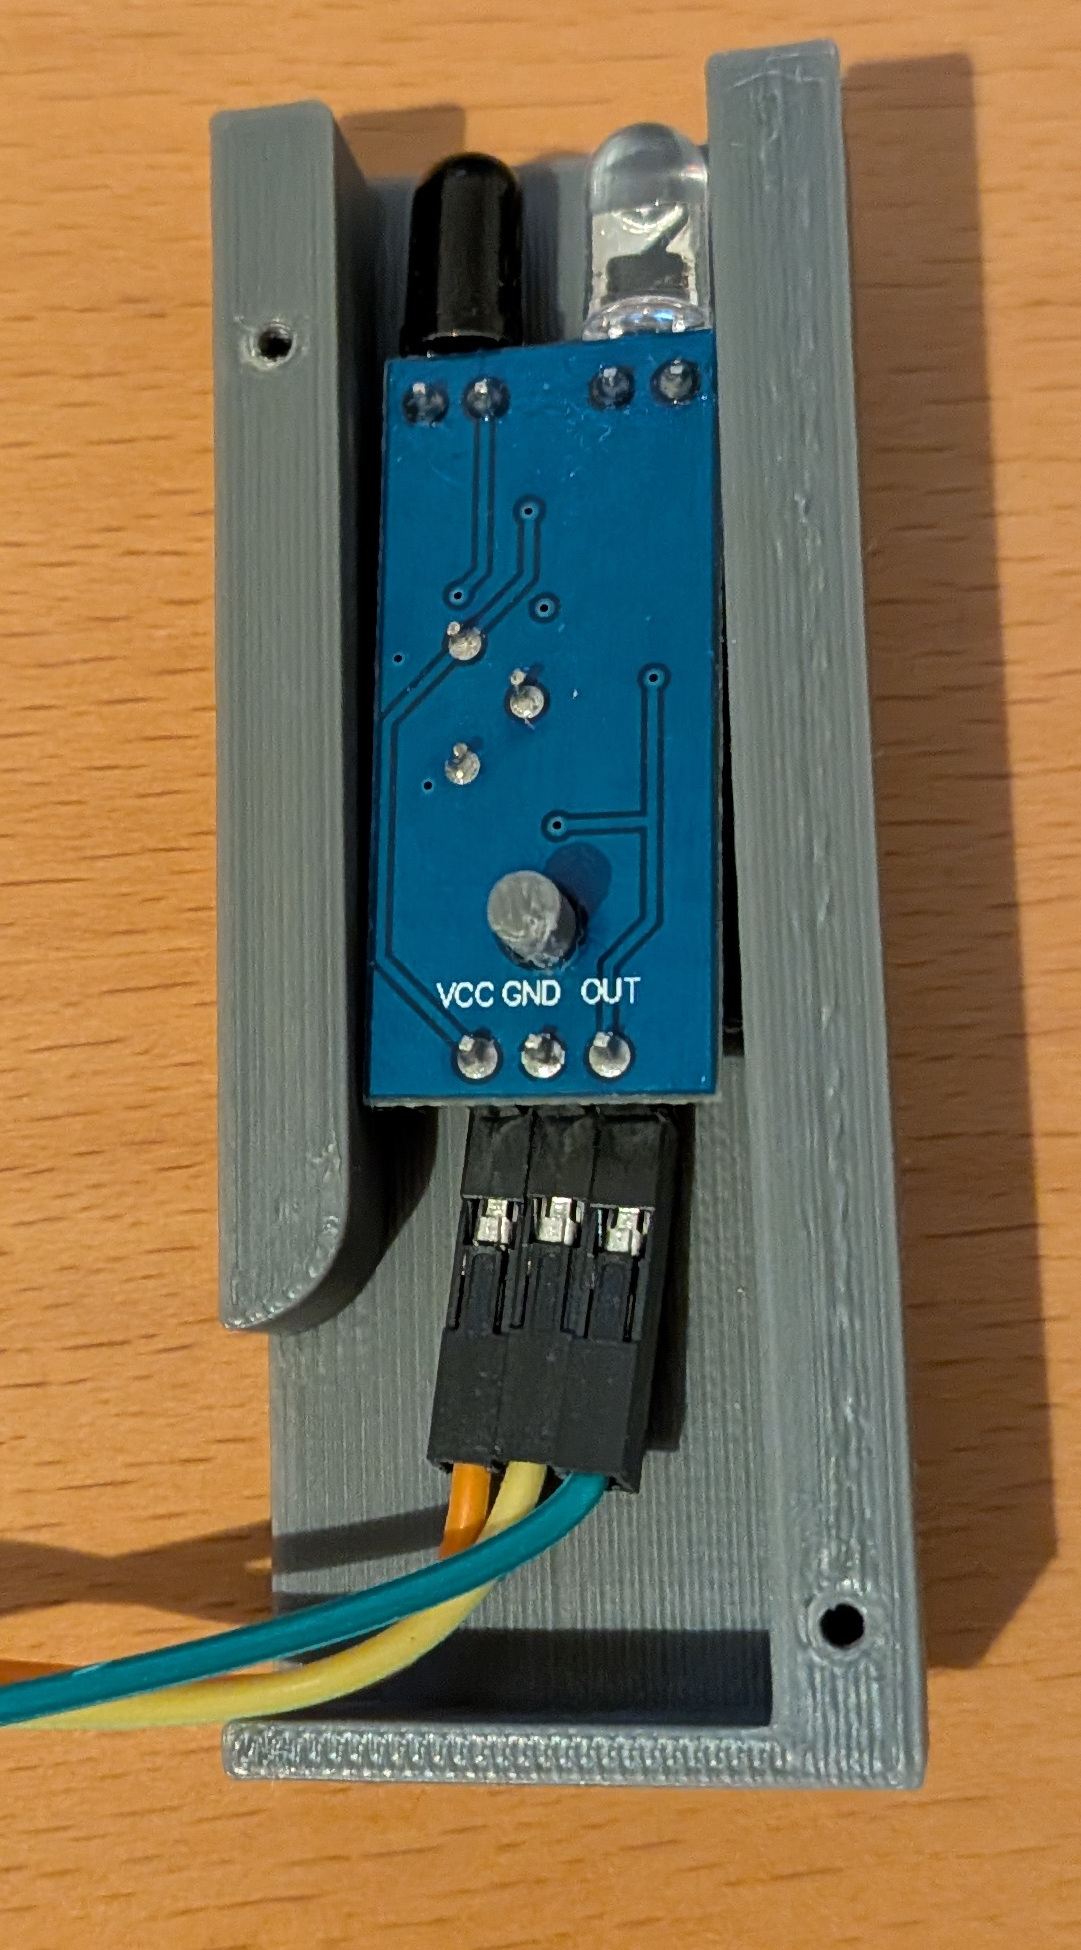
\includegraphics[scale=0.08]{montage_gereon/tischkantensensor/PXL_20260907_153439687.jpg}

Nun wird die Abdeckplatte auf dem Träger platziert und rückseitig verschraubt. Das Poti zur Empfindlichkeitsregelung muss dabei in der Aussparung sichtbar sein.

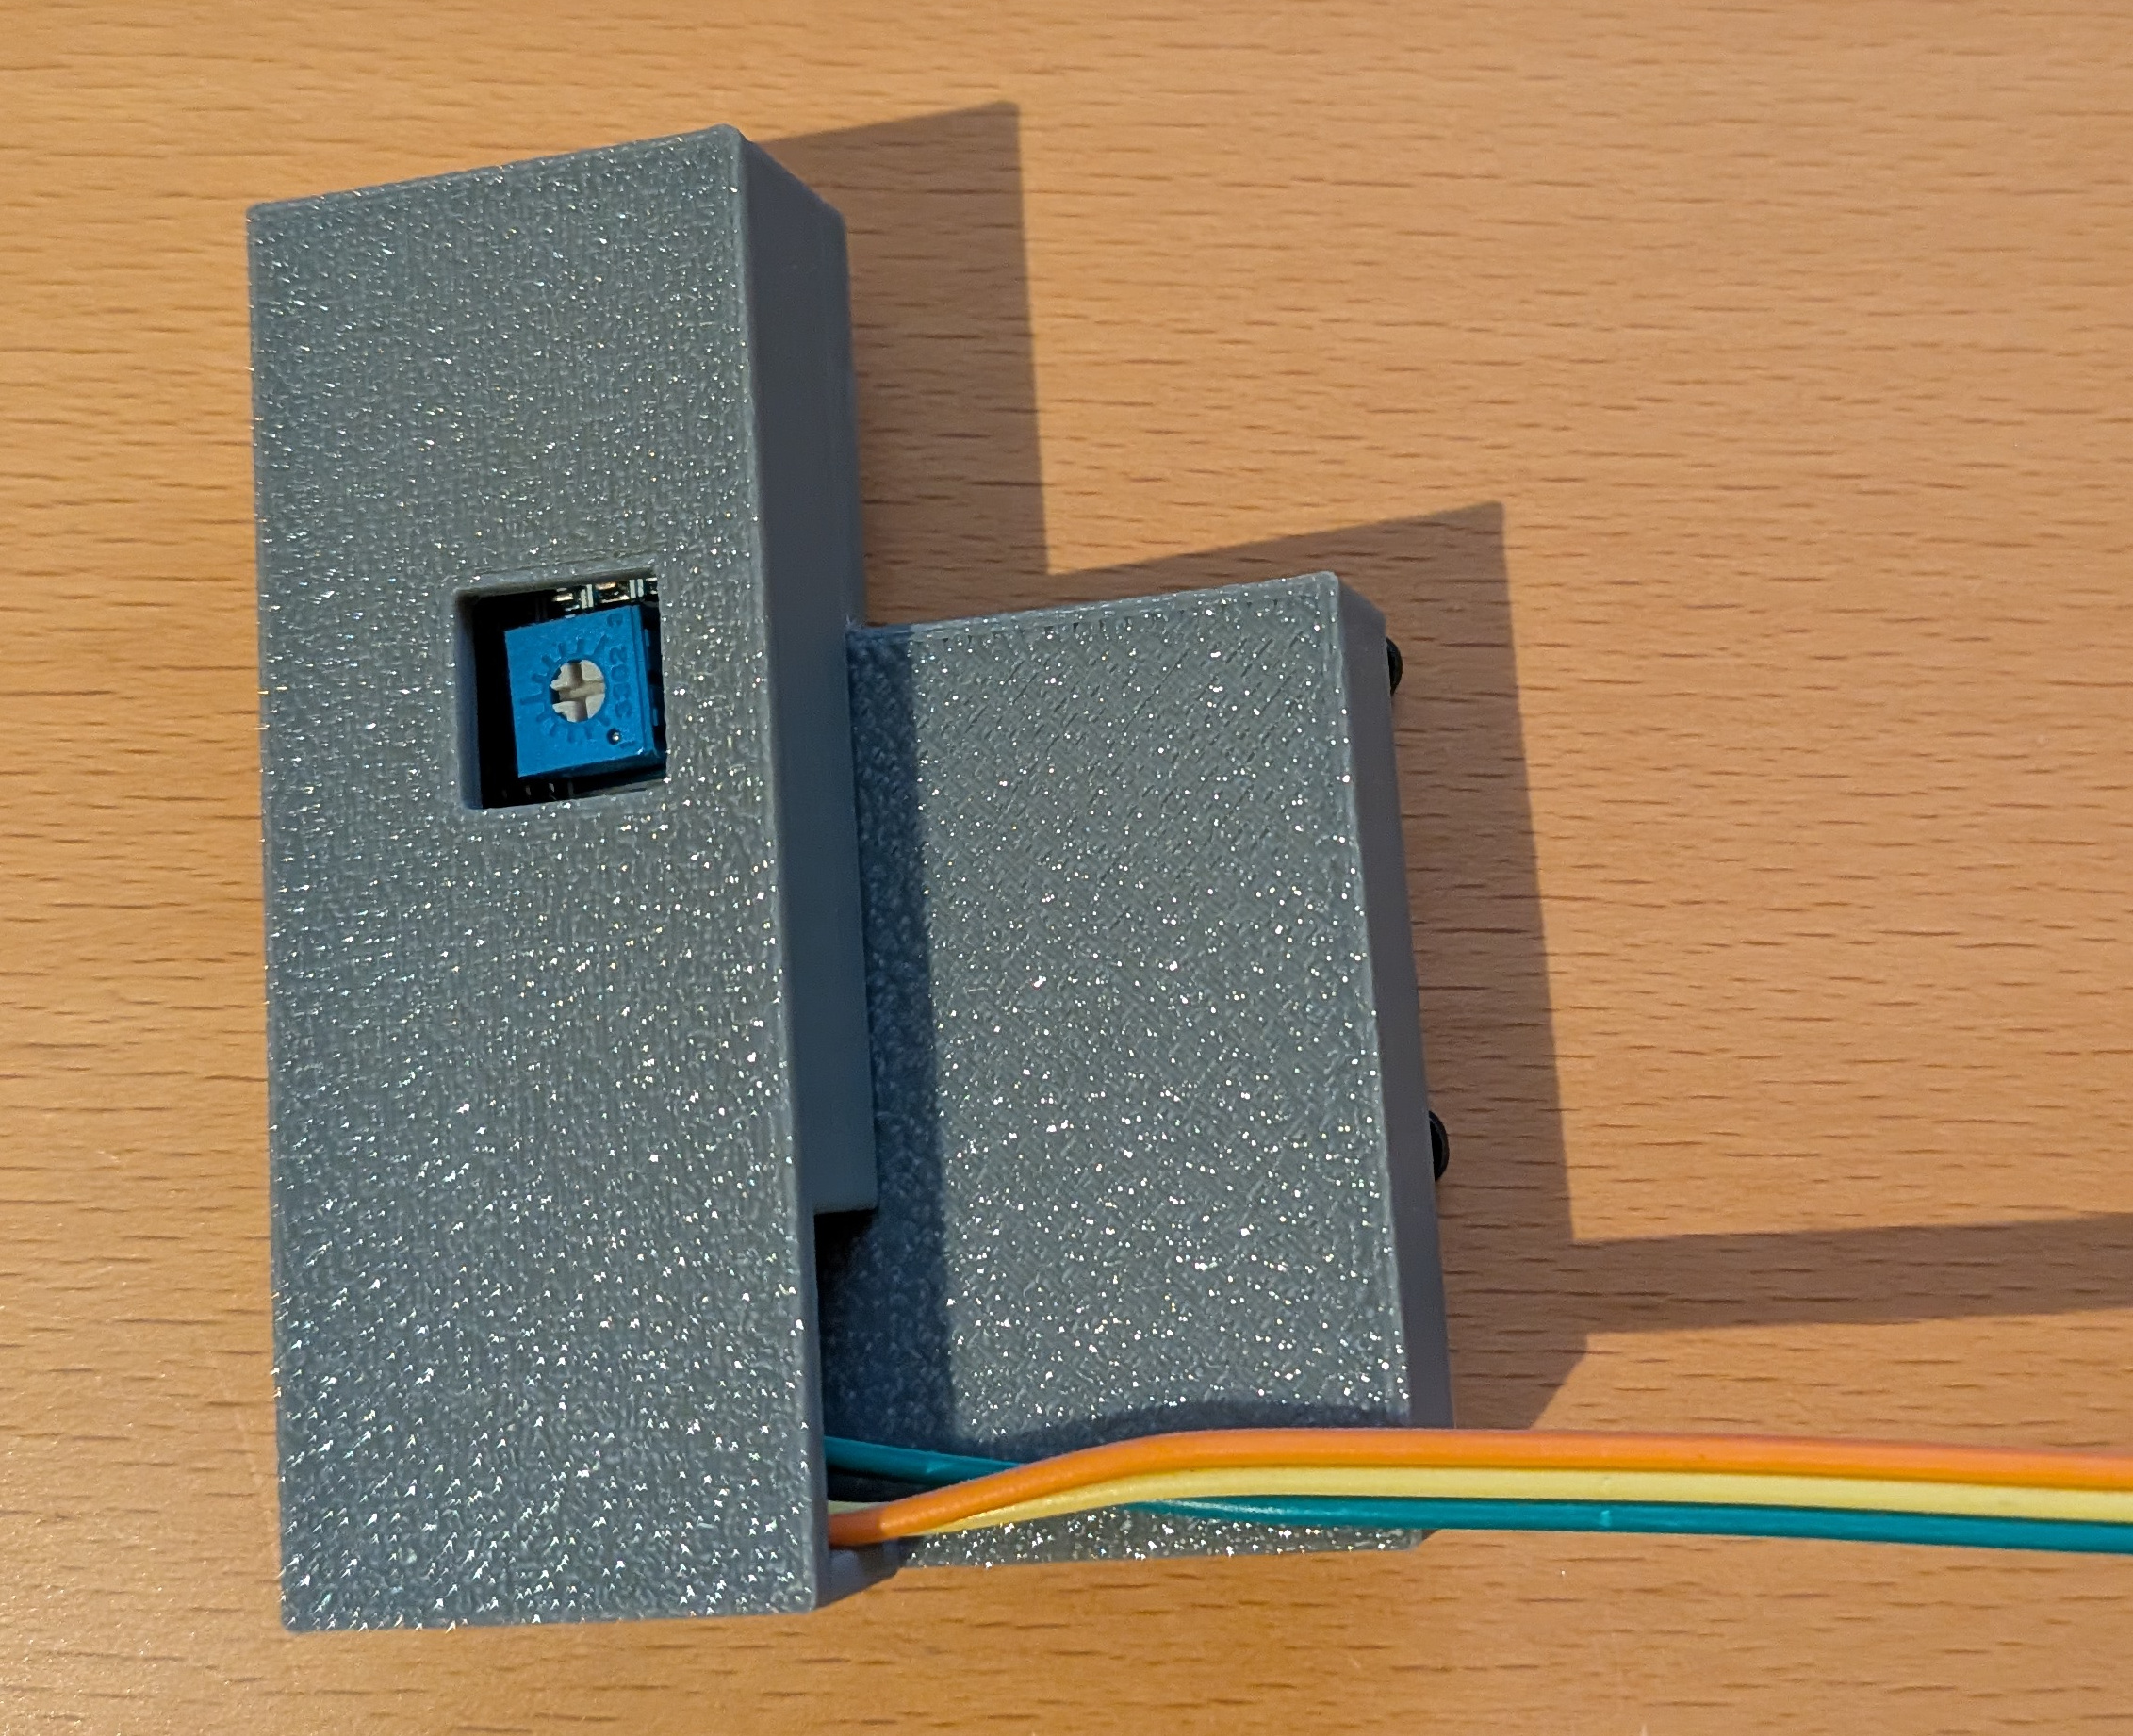
\includegraphics[scale=0.08]{montage_gereon/tischkantensensor/PXL_20260912_182526907.jpg}



\subsubsection{Kollisionserkennung}

Zur montage des Ultraschall Sensors wird dieser zunächst im Gehäuse platziert und fixiert

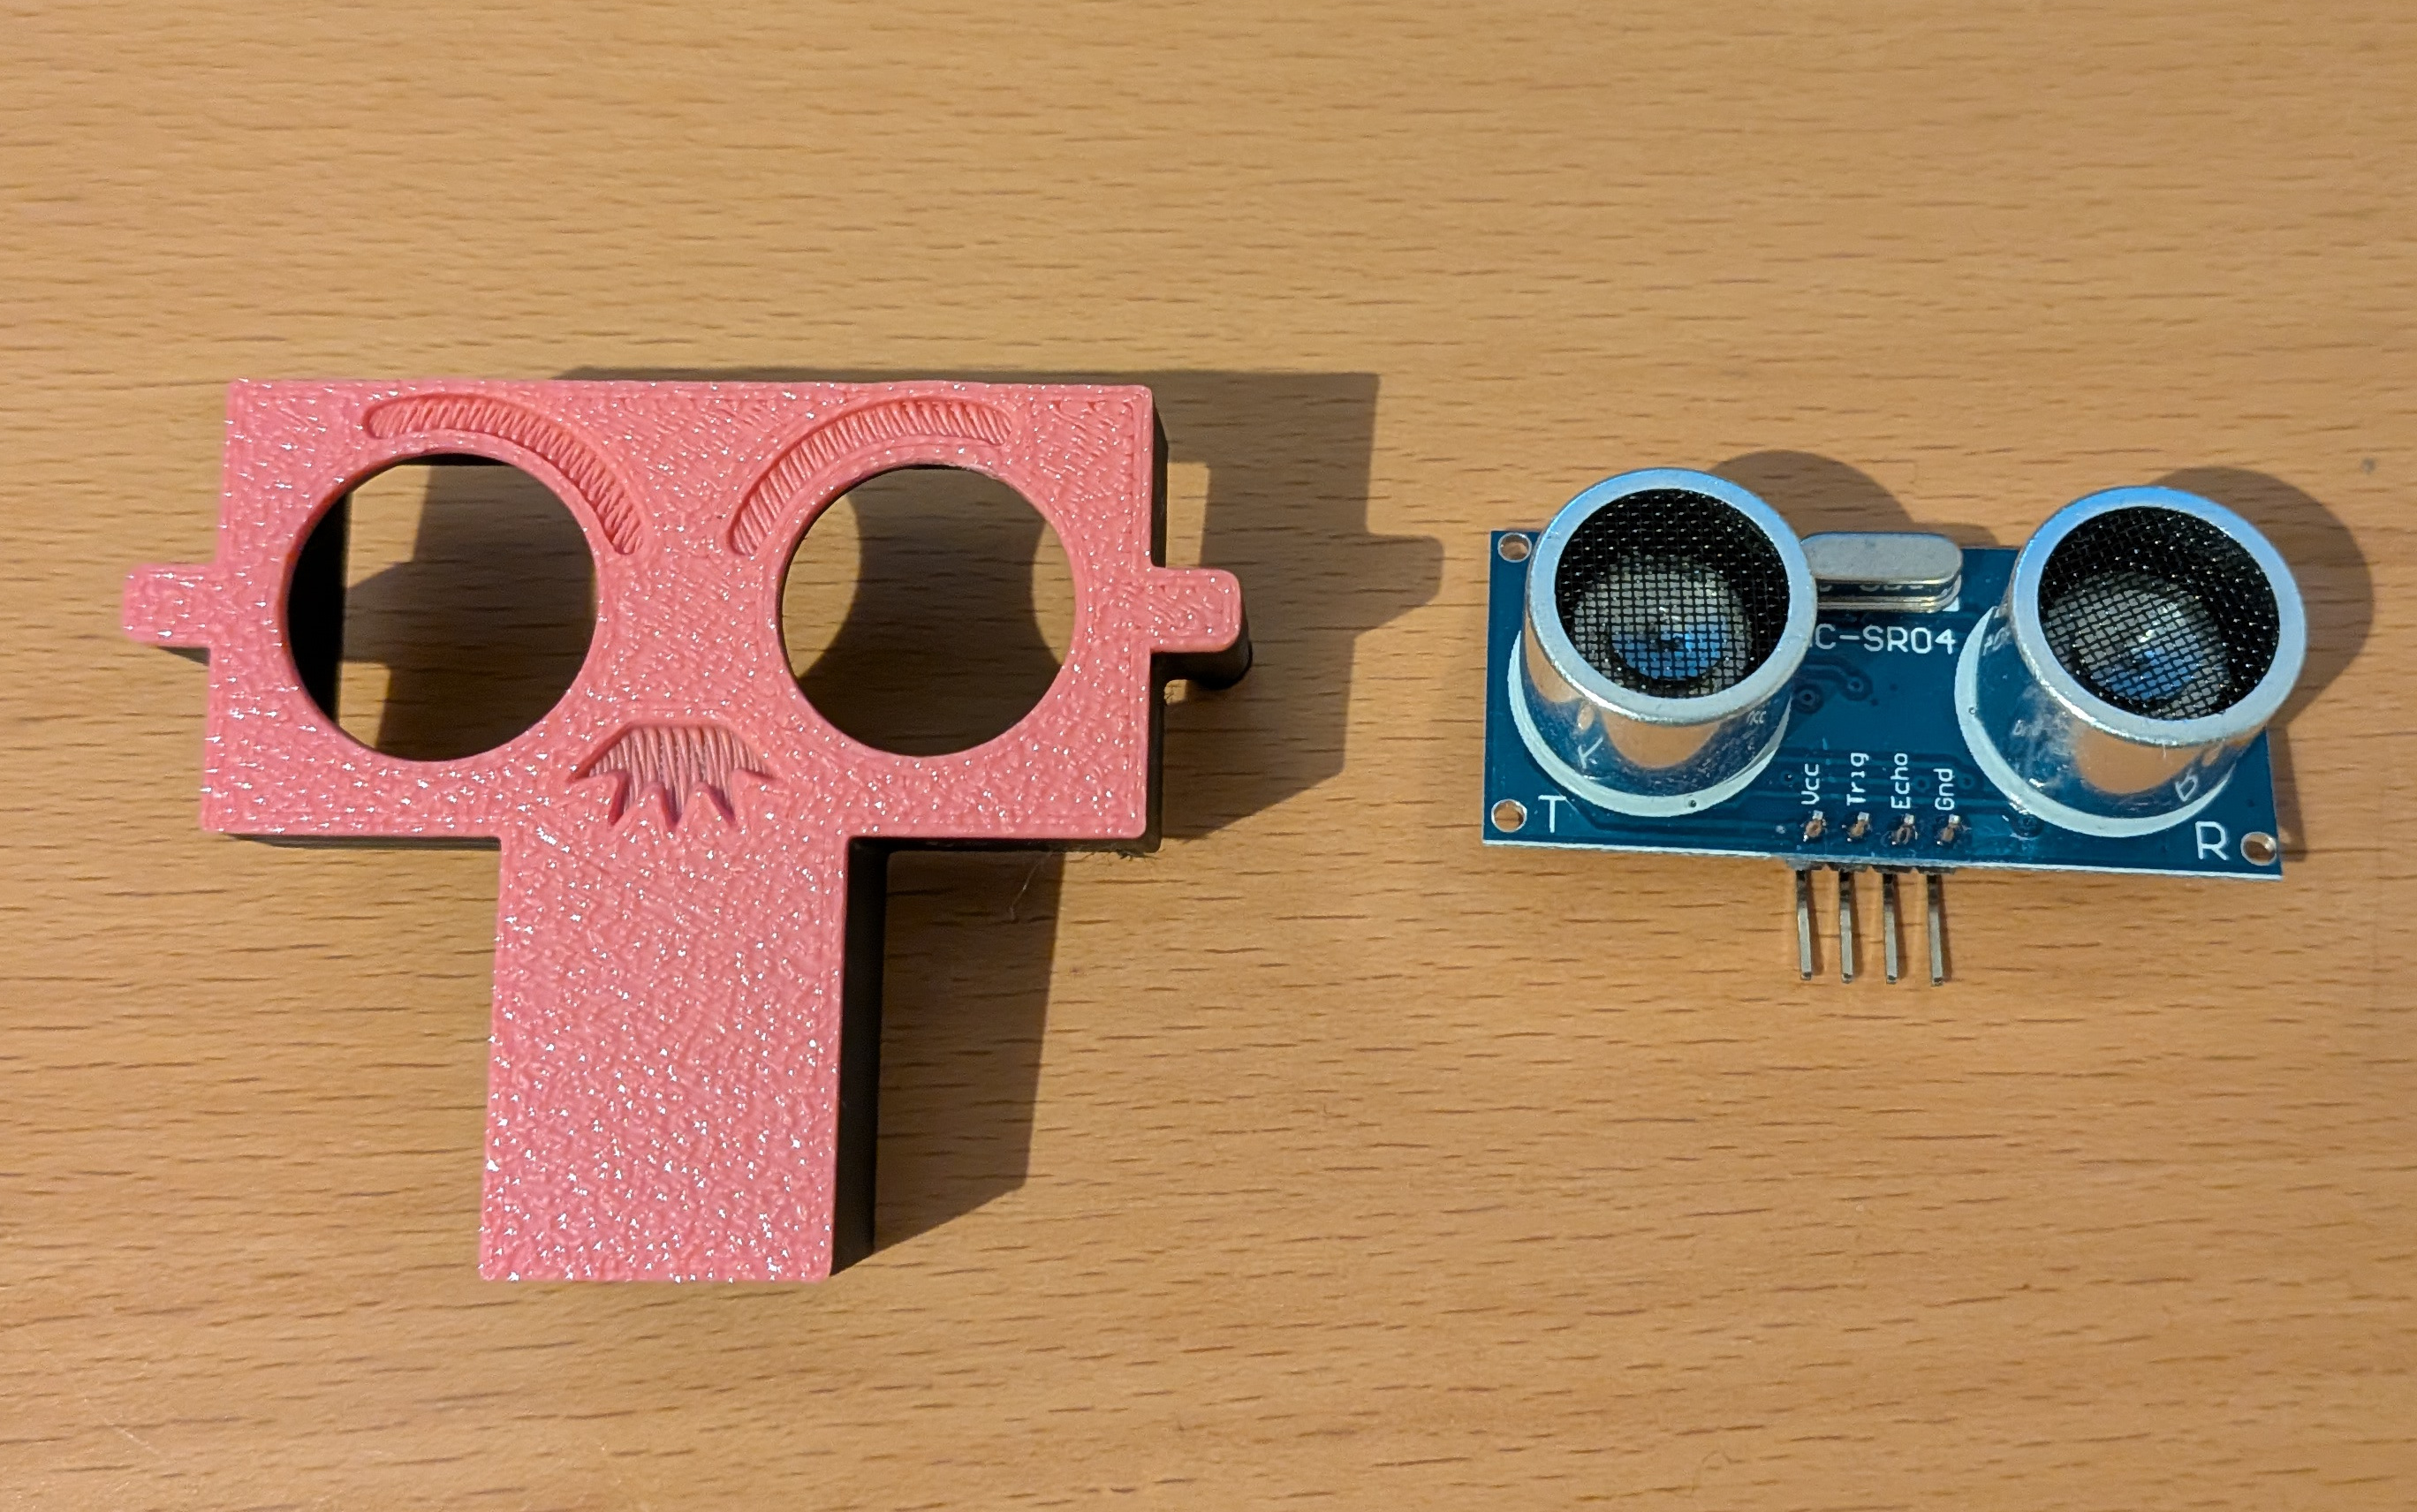
\includegraphics[scale=0.08]{montage_gereon/echo_sensor/PXL_20260907_152931739.jpg}
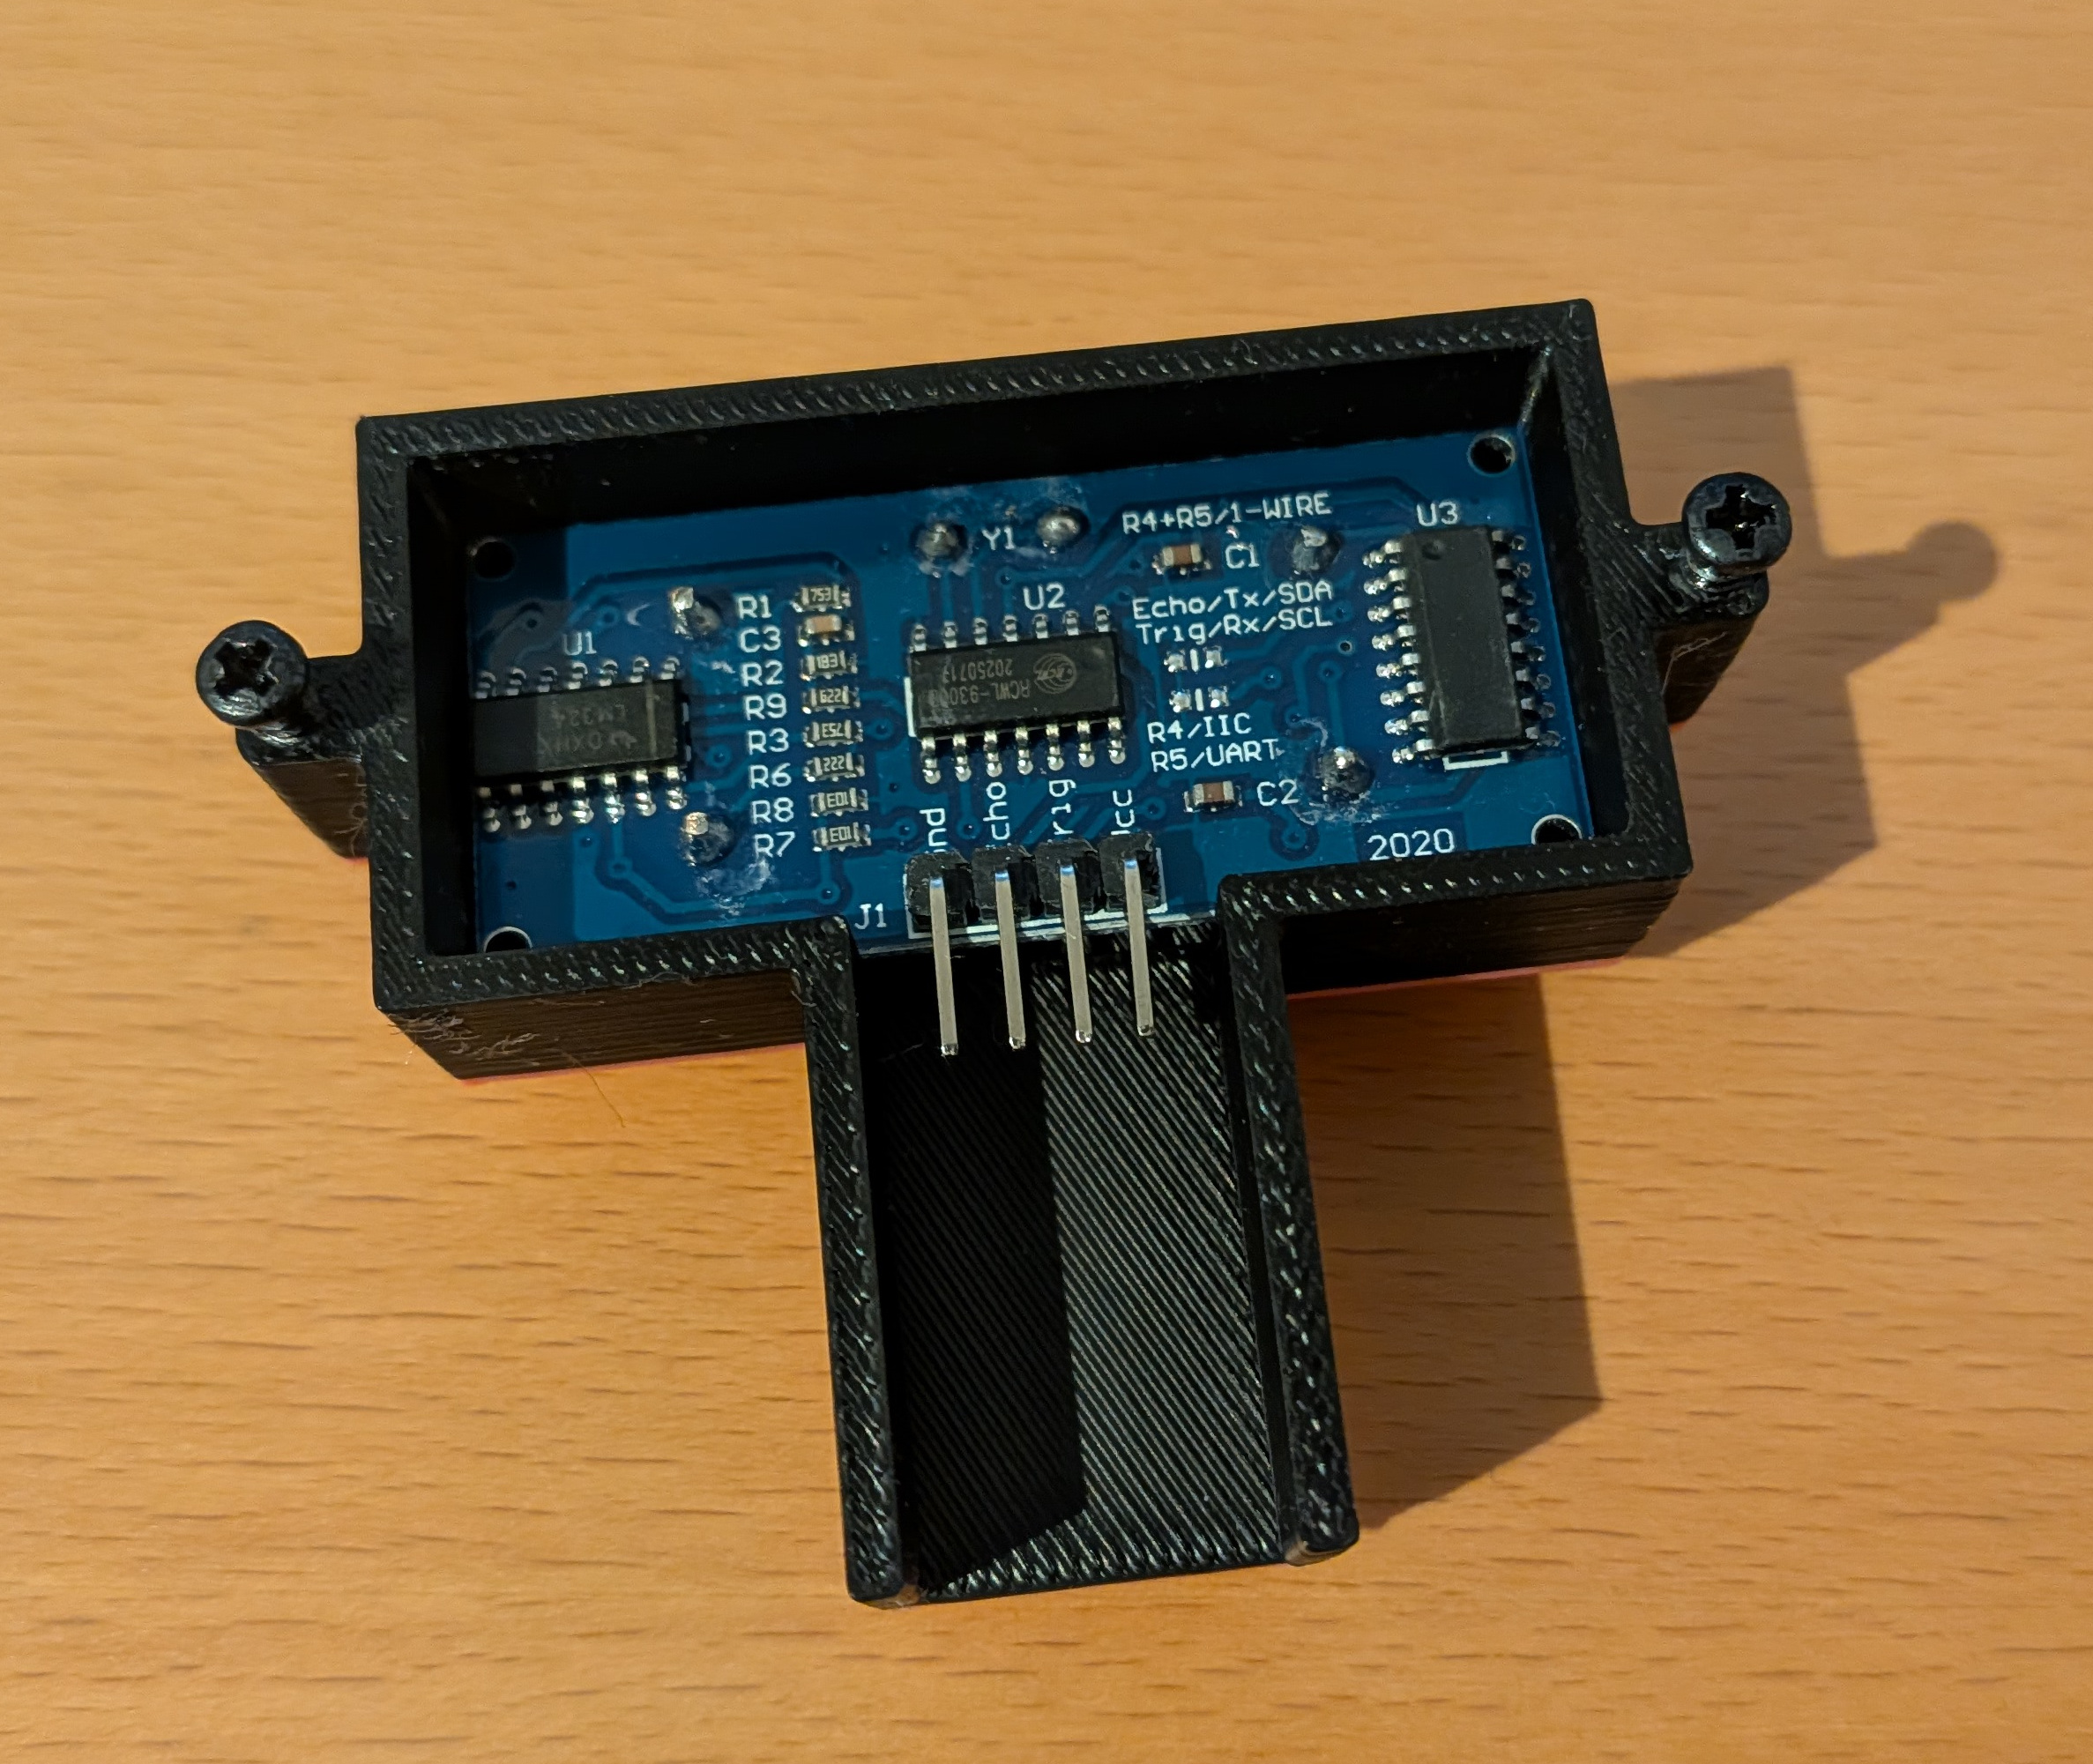
\includegraphics[scale=0.08]{montage_gereon/echo_sensor/PXL_20260907_152946157.jpg}

Anschließend wird das vieradrige Flachbandlabel mit der Sensorplatine verbunden:

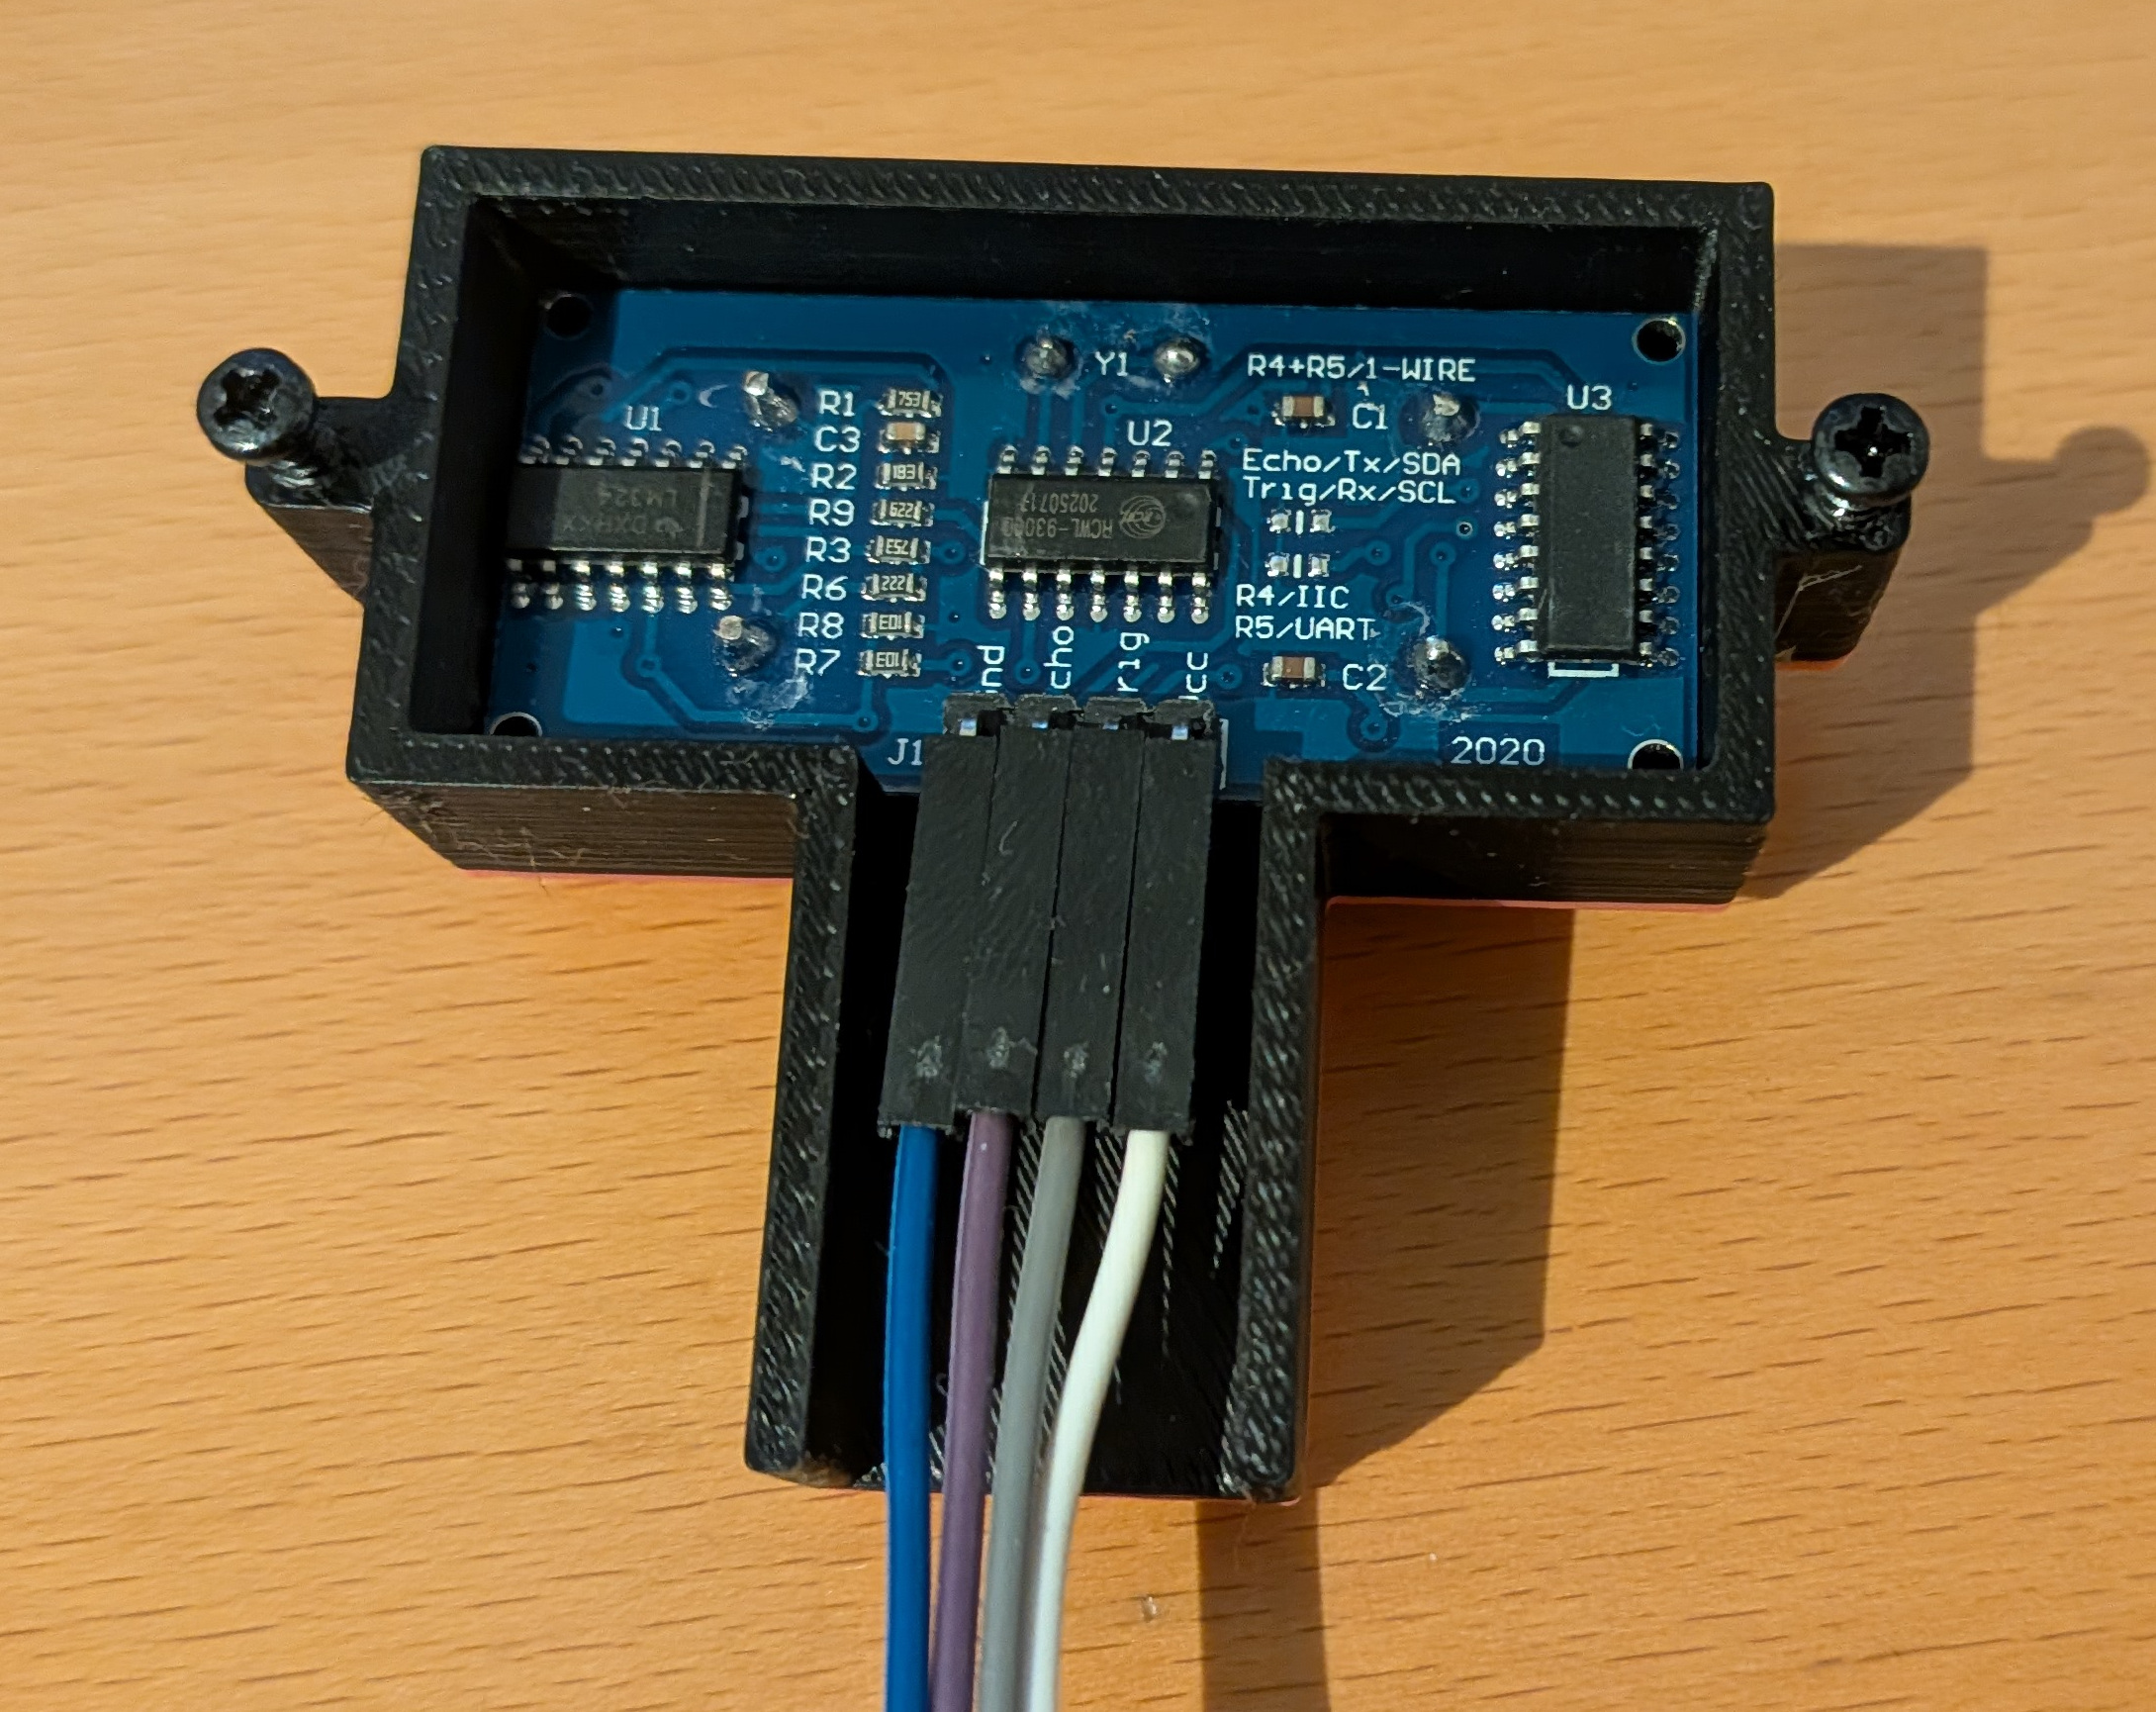
\includegraphics[scale=0.08]{montage_gereon/echo_sensor/PXL_20260907_153137301.jpg}

Nun wird das Ultraschallmodul auf der Frontplatte montiert.

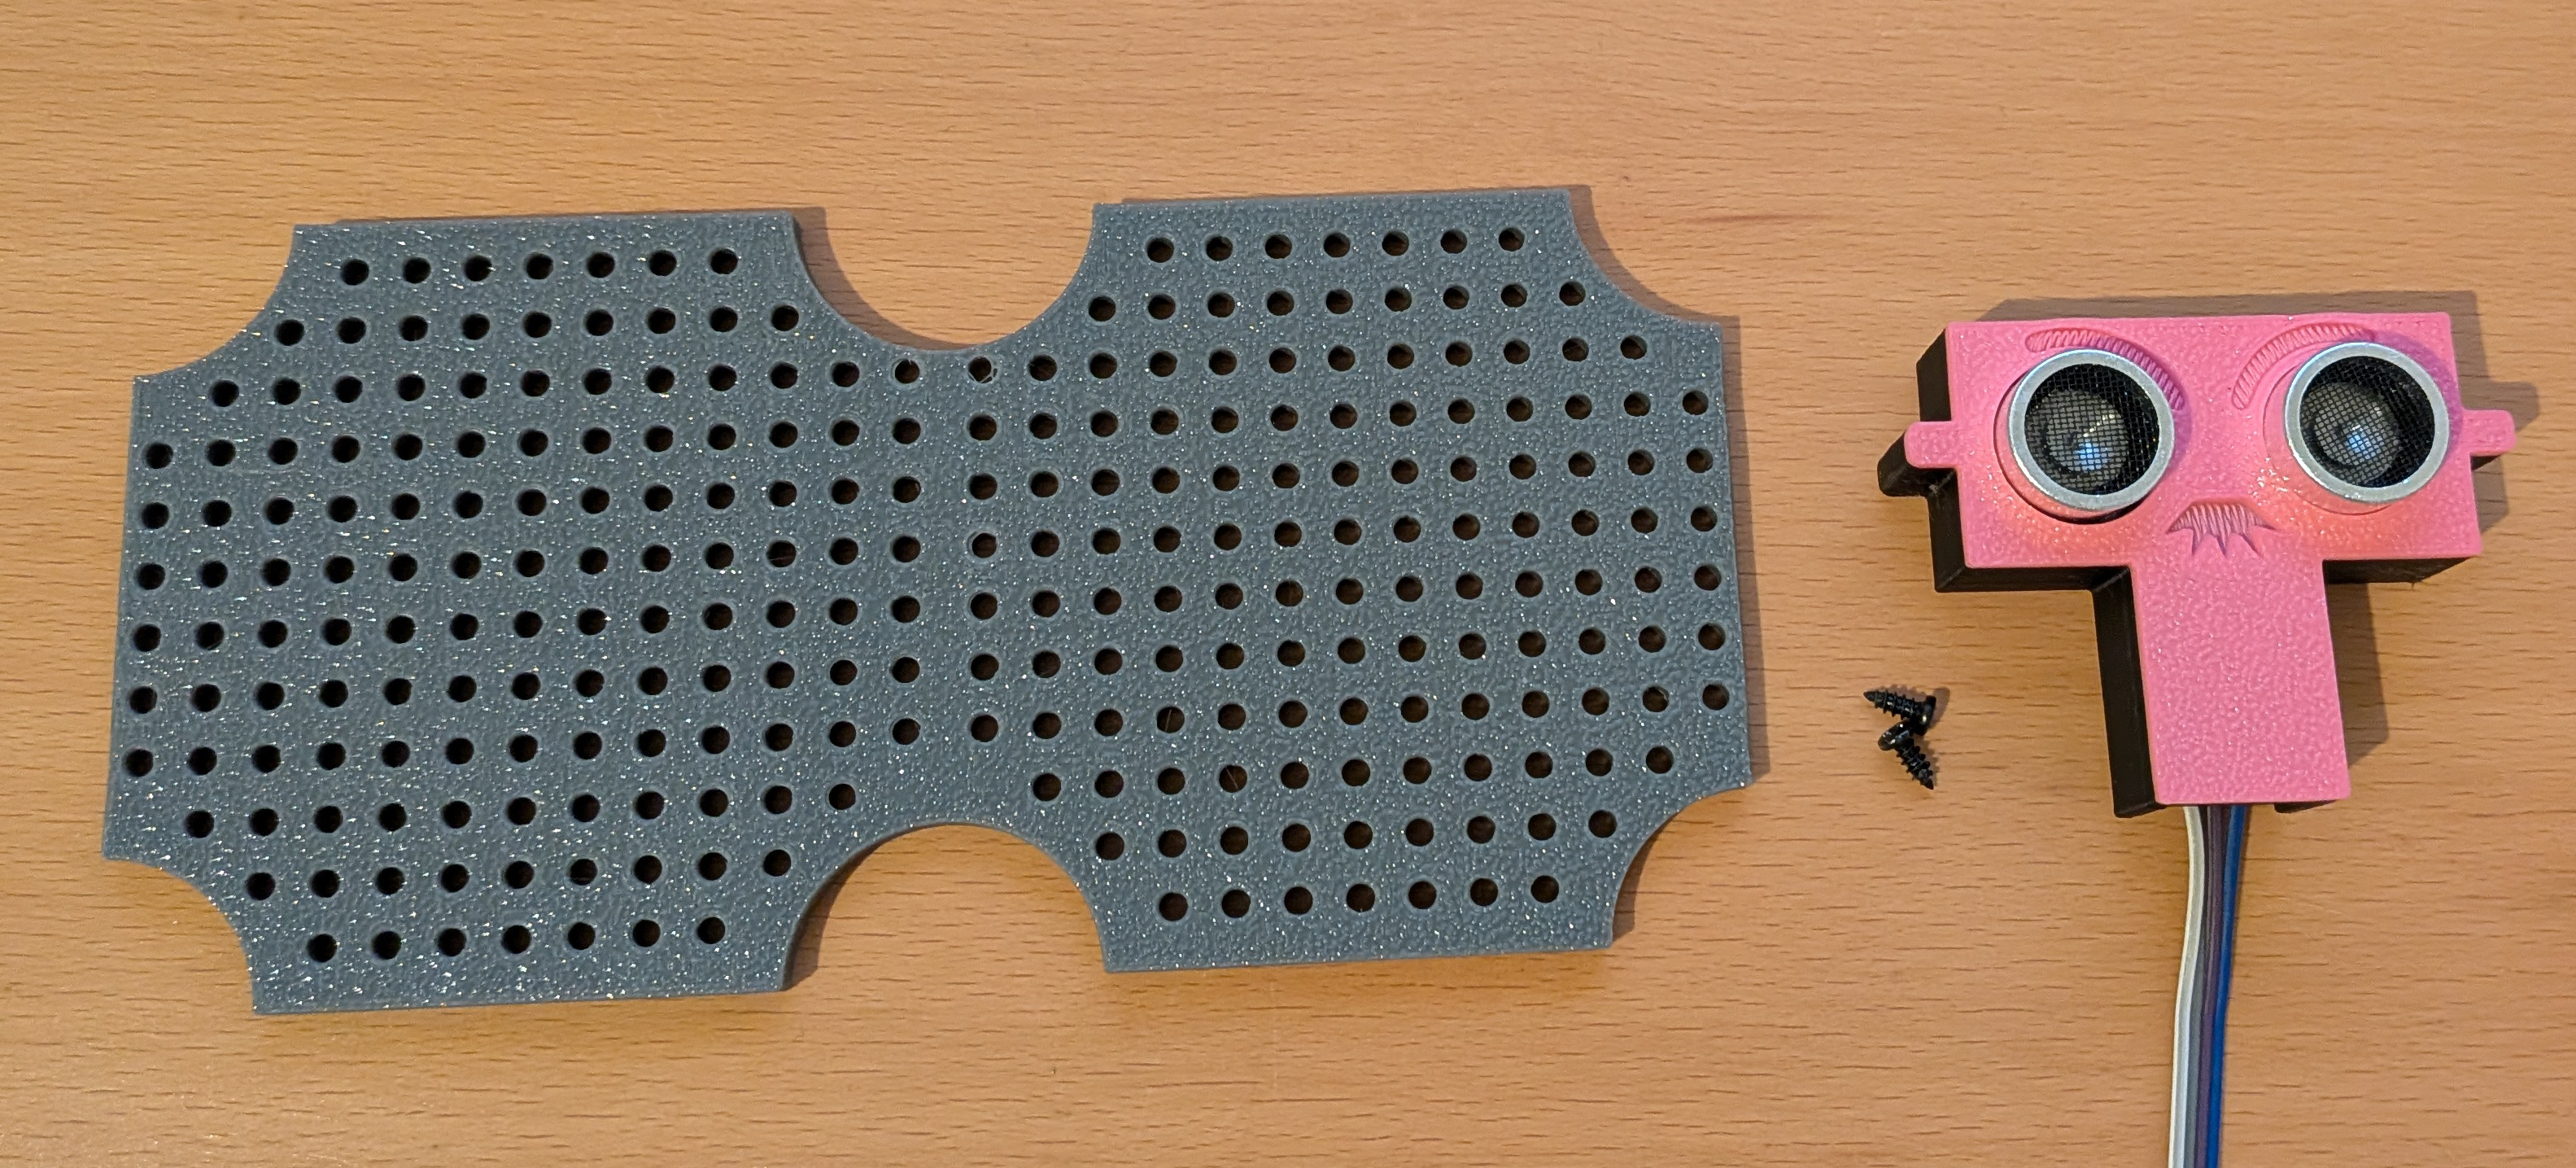
\includegraphics[scale=0.08]{montage_gereon/echo_sensor/PXL_20260912_185729773.jpg}

Dazu wird das Gehäuse rückseitig mit der mittleren Lochreihe verschraubt. Das Gehäuse des Ultraschall Sensors sollte nun bündig mit der Unterseite der vorderen Außenwand sein, unmittelbar vor der Kabeldurchfürung. 

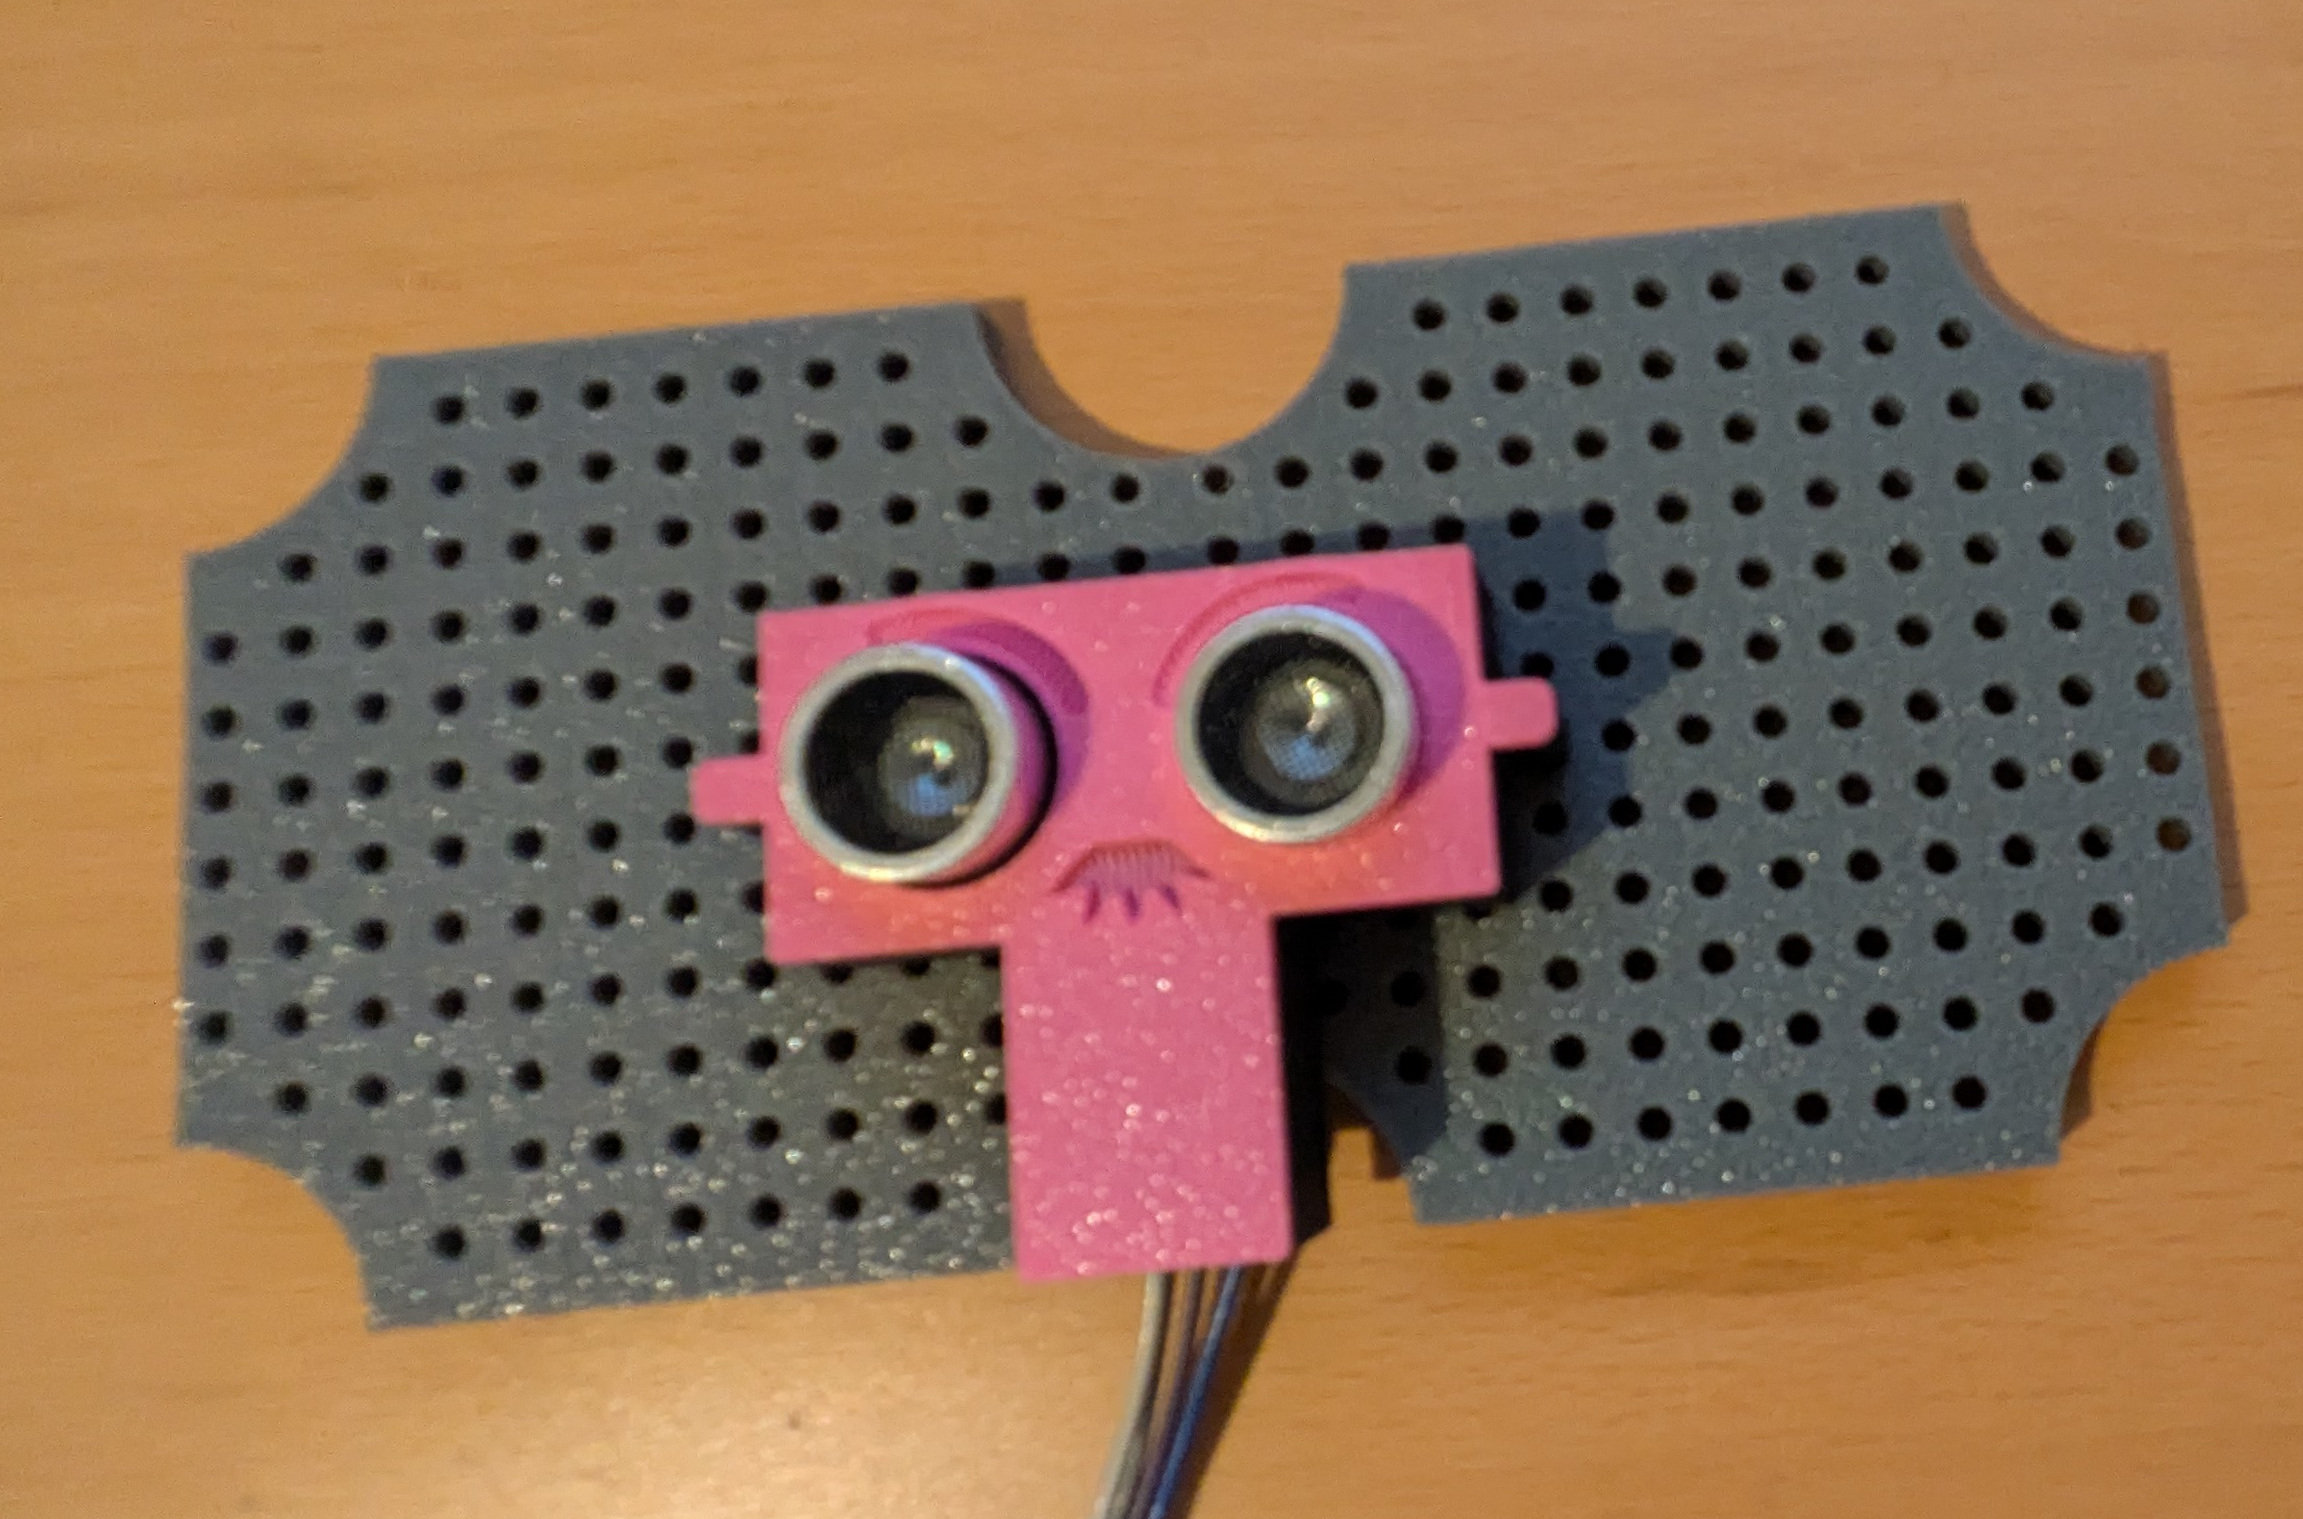
\includegraphics[scale=0.08]{montage_gereon/echo_sensor/PXL_20260912_185912814.jpg}
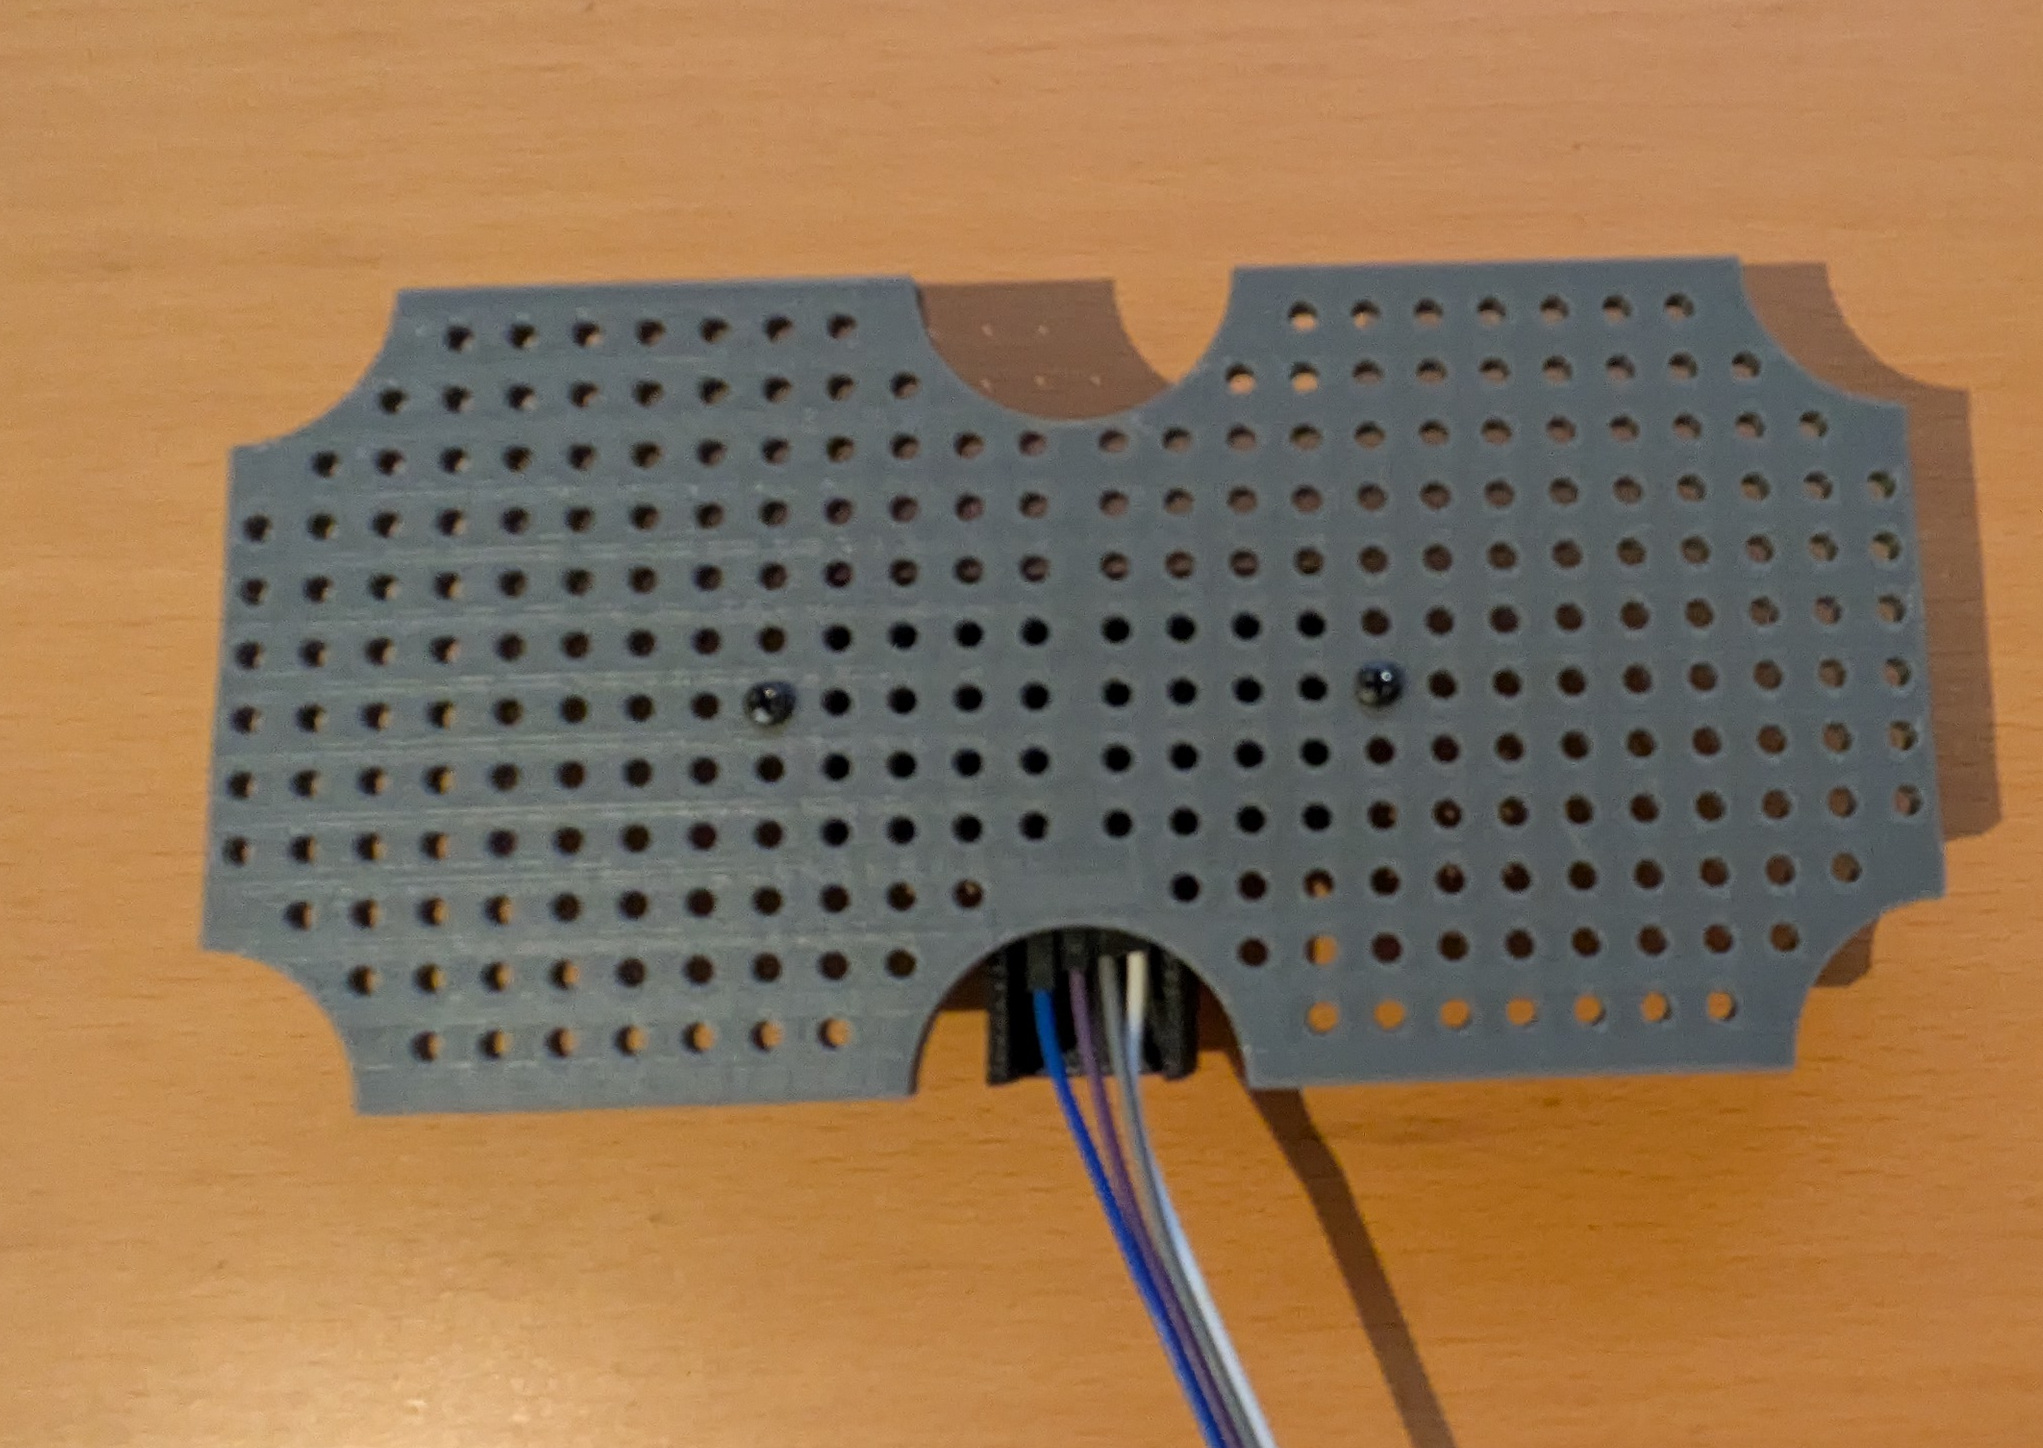
\includegraphics[scale=0.08]{montage_gereon/echo_sensor/PXL_20260912_185907017.jpg}






\subsection{Antriebs-Aktorik montieren}

Nun erfolgt die Montage der DC Antriebsmotoren

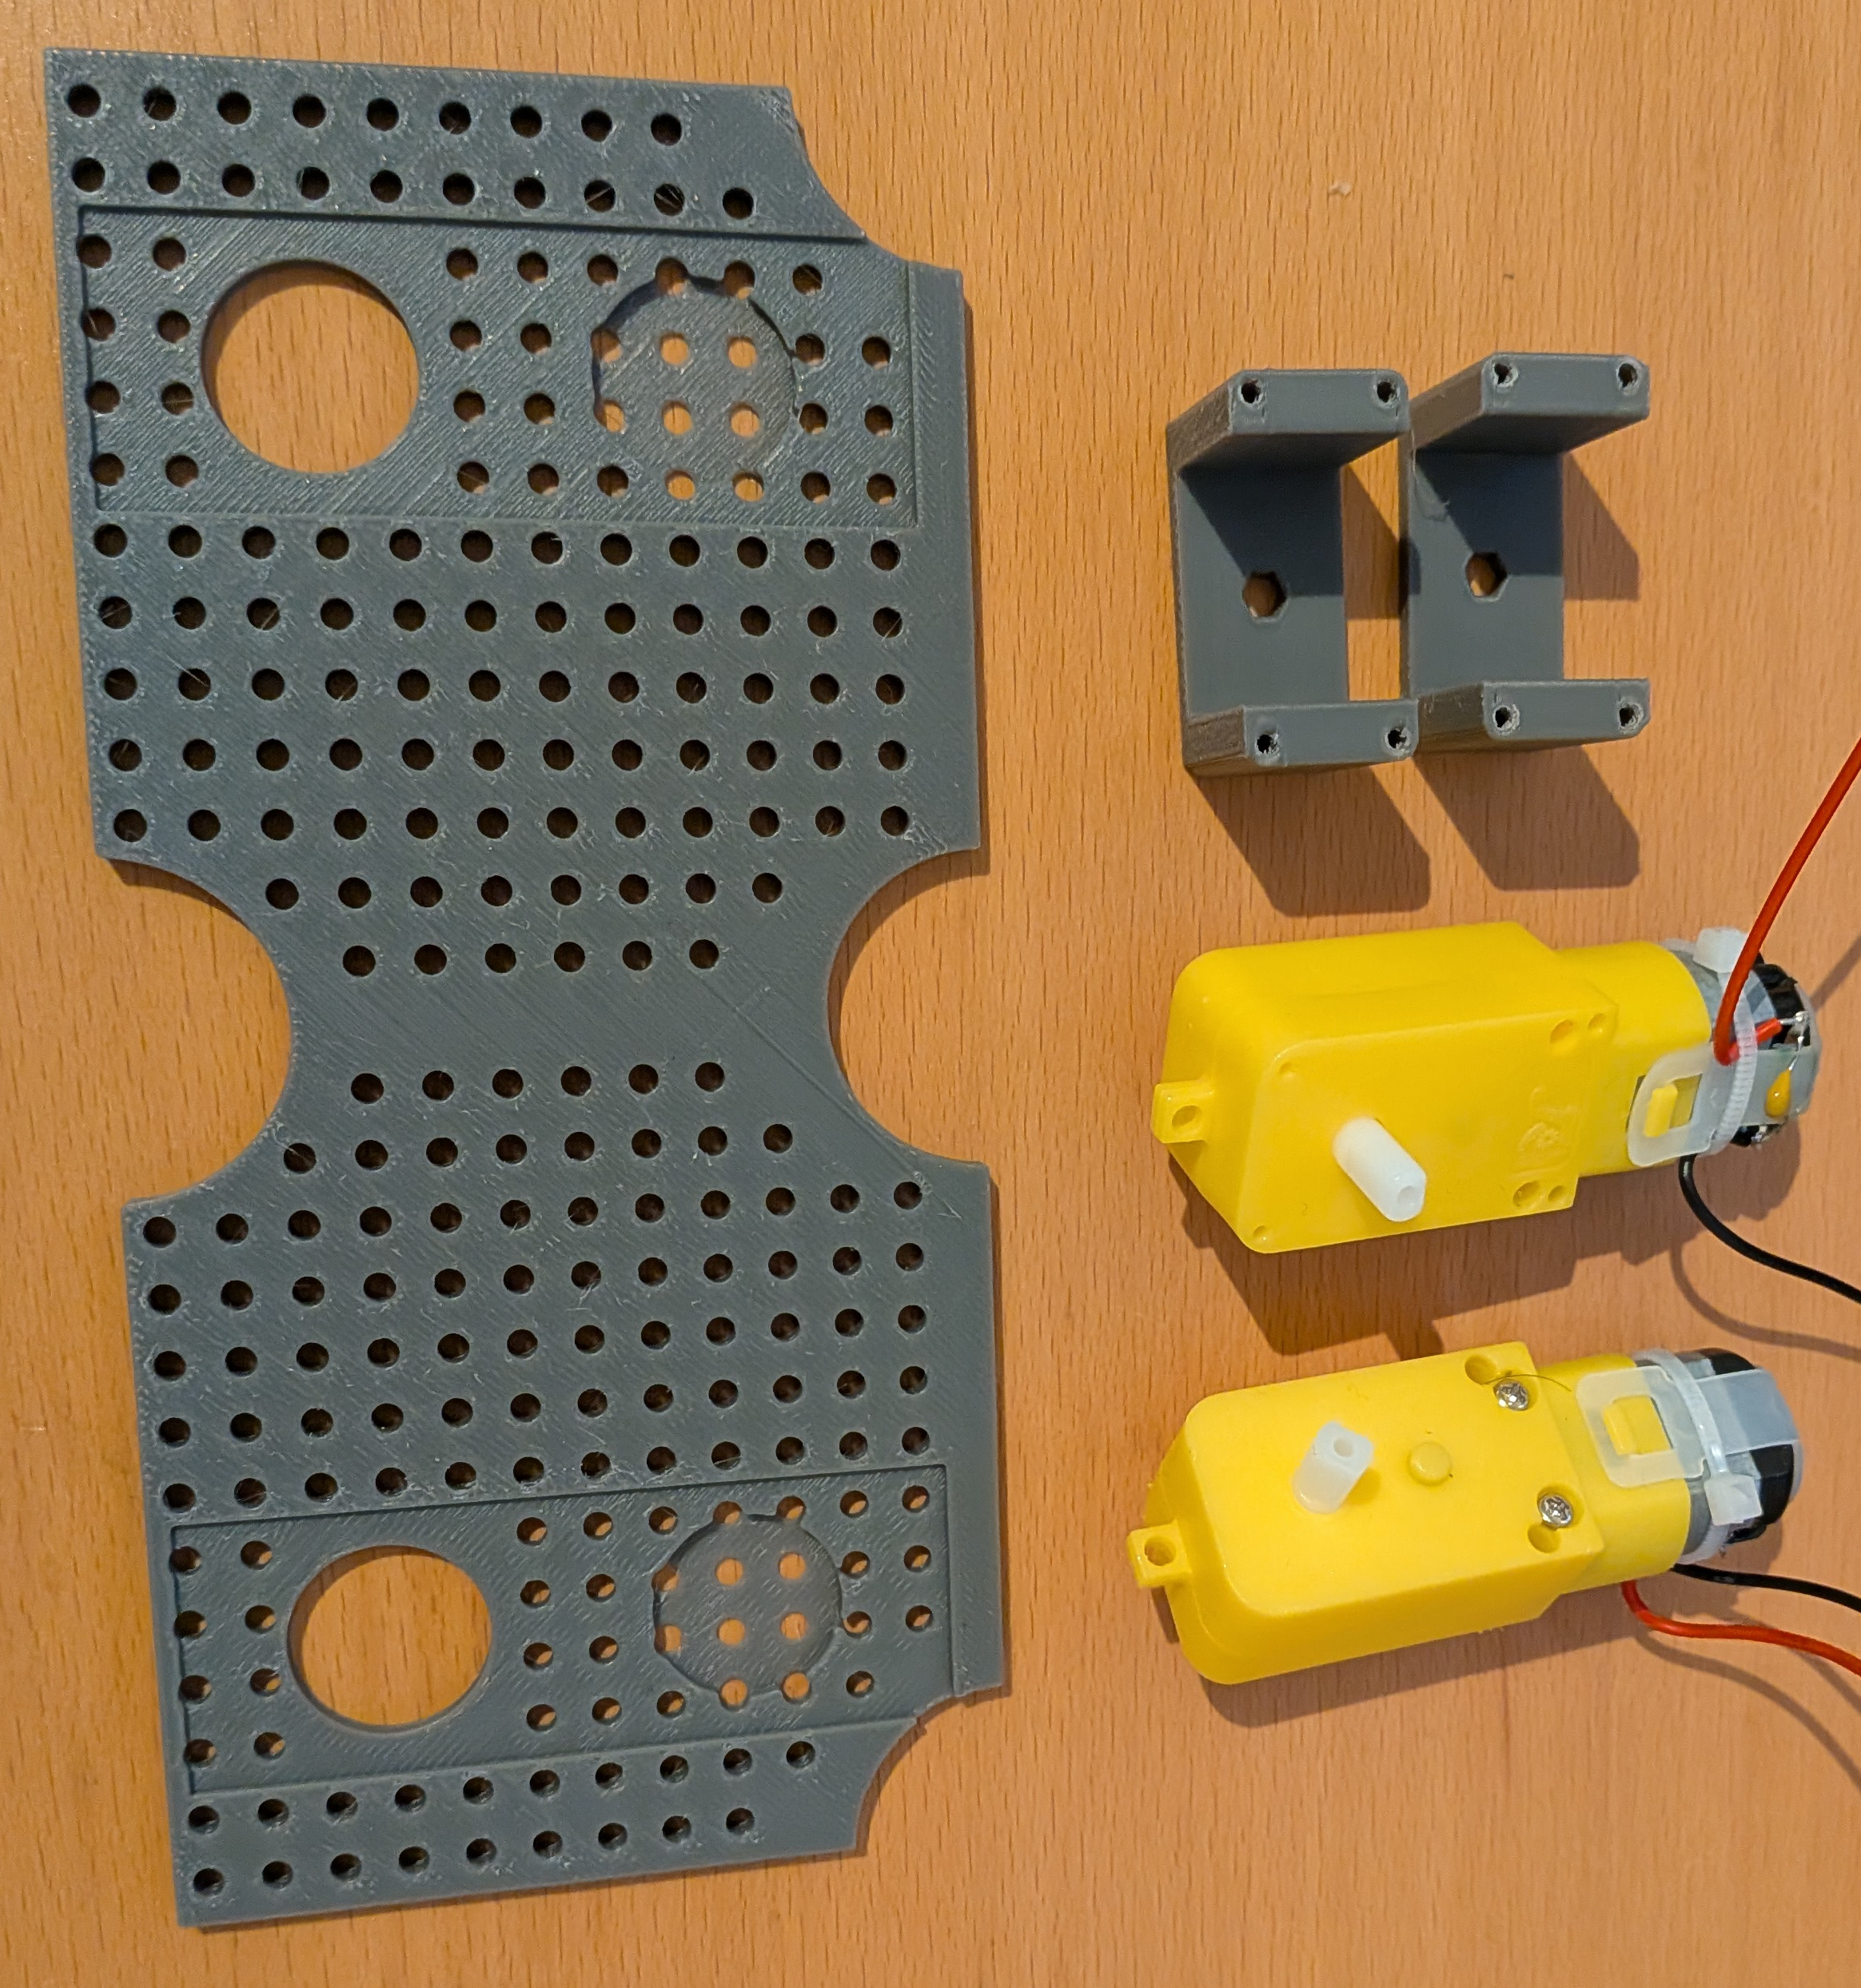
\includegraphics[scale=0.08]{montage_gereon/antrieb_montage/PXL_20260907_162144293.jpg}

Falls noch nicht erfolgt bzw. im genutzten Motormodell nicht ohnehin vorhanden werden zunächst an den TT Motoren über die Lötfahnen die 100nF Kondensatoren zum Entstören gelötet. 

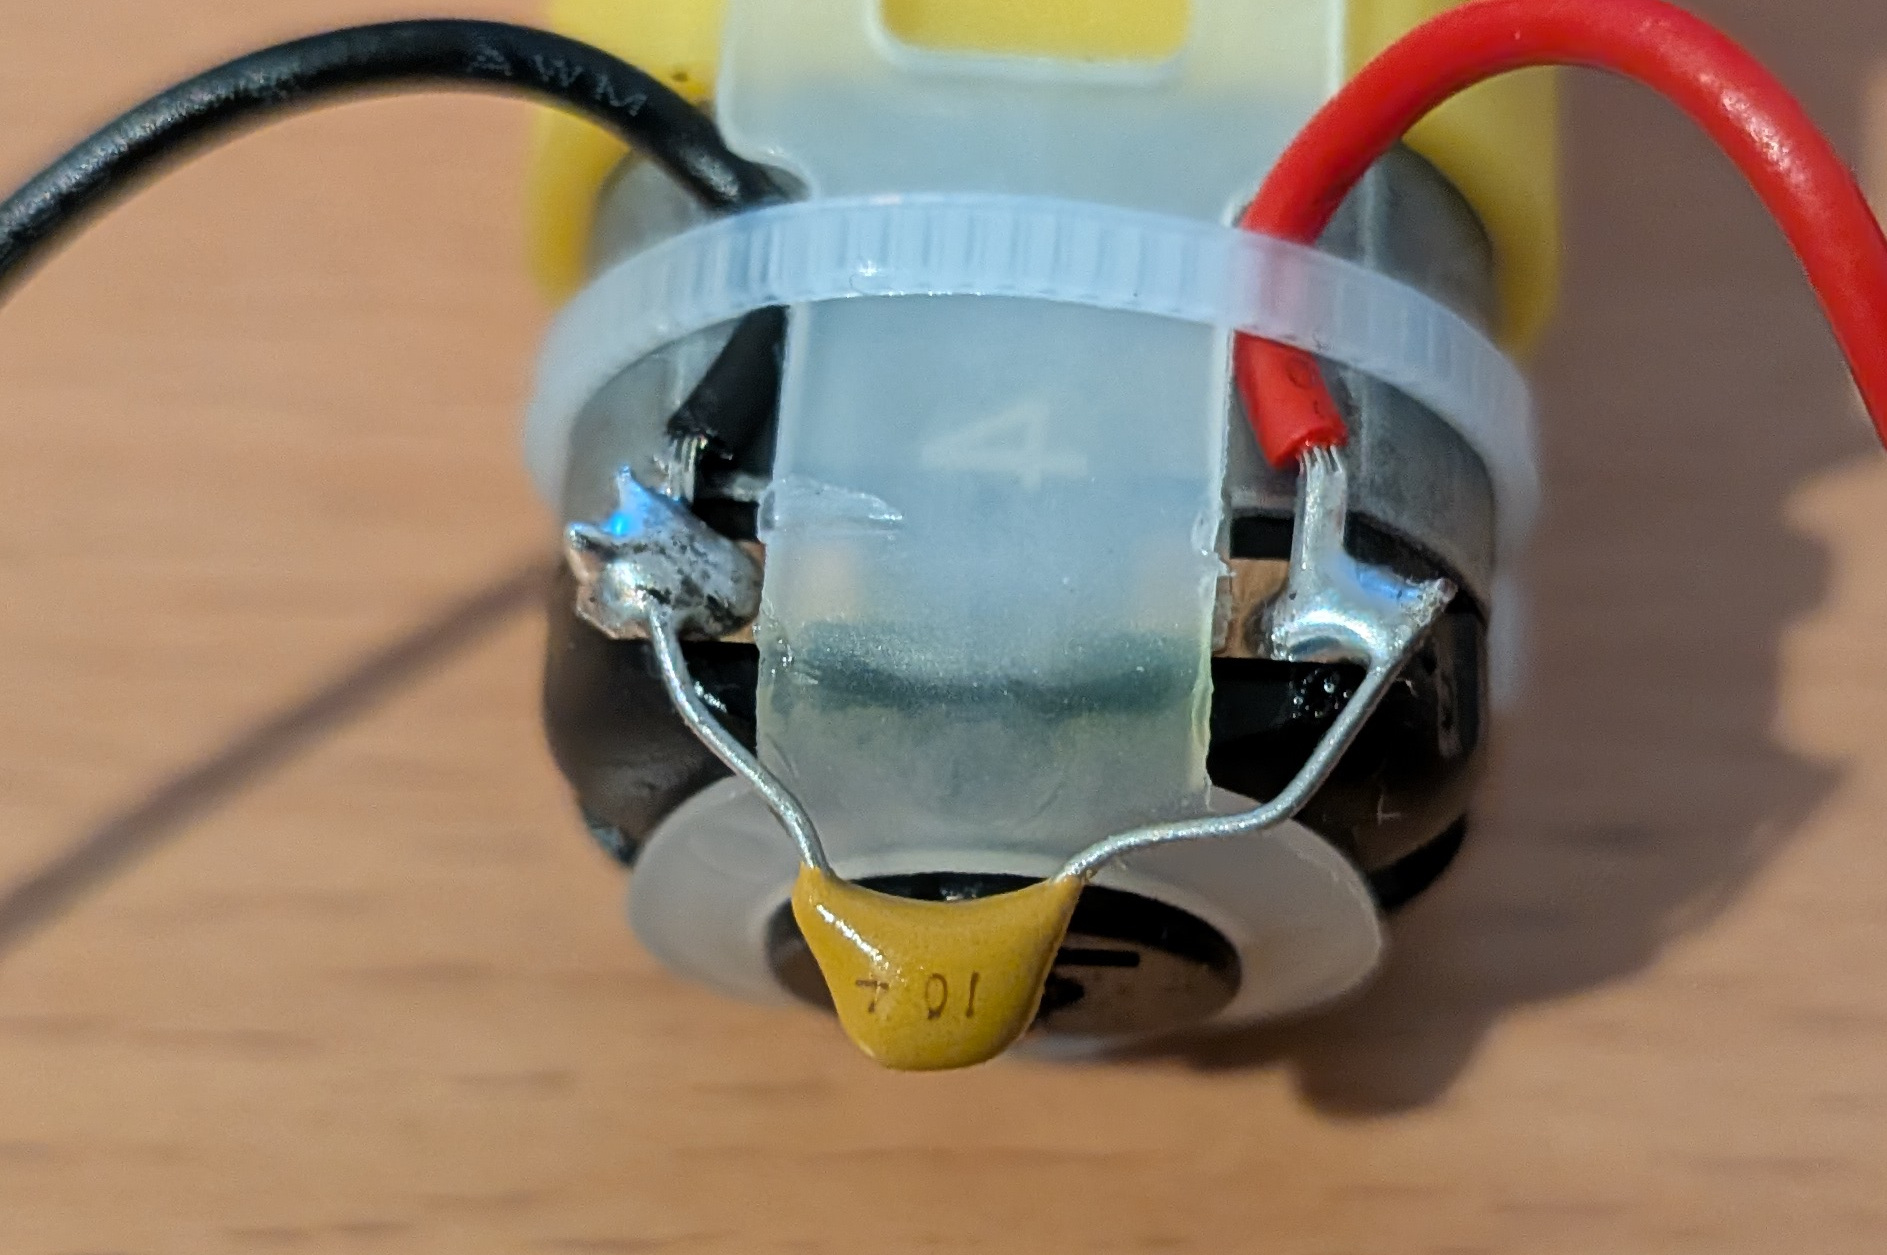
\includegraphics[scale=0.1]{montage_gereon/antrieb_montage/PXL_20260909_081137444.jpg}


\begin{warnbox}
Die Kondensatoren müssen nach oben gerichtet werden, ansonsten lässt sich der Motor nicht bündig am gehäuse fixieren.

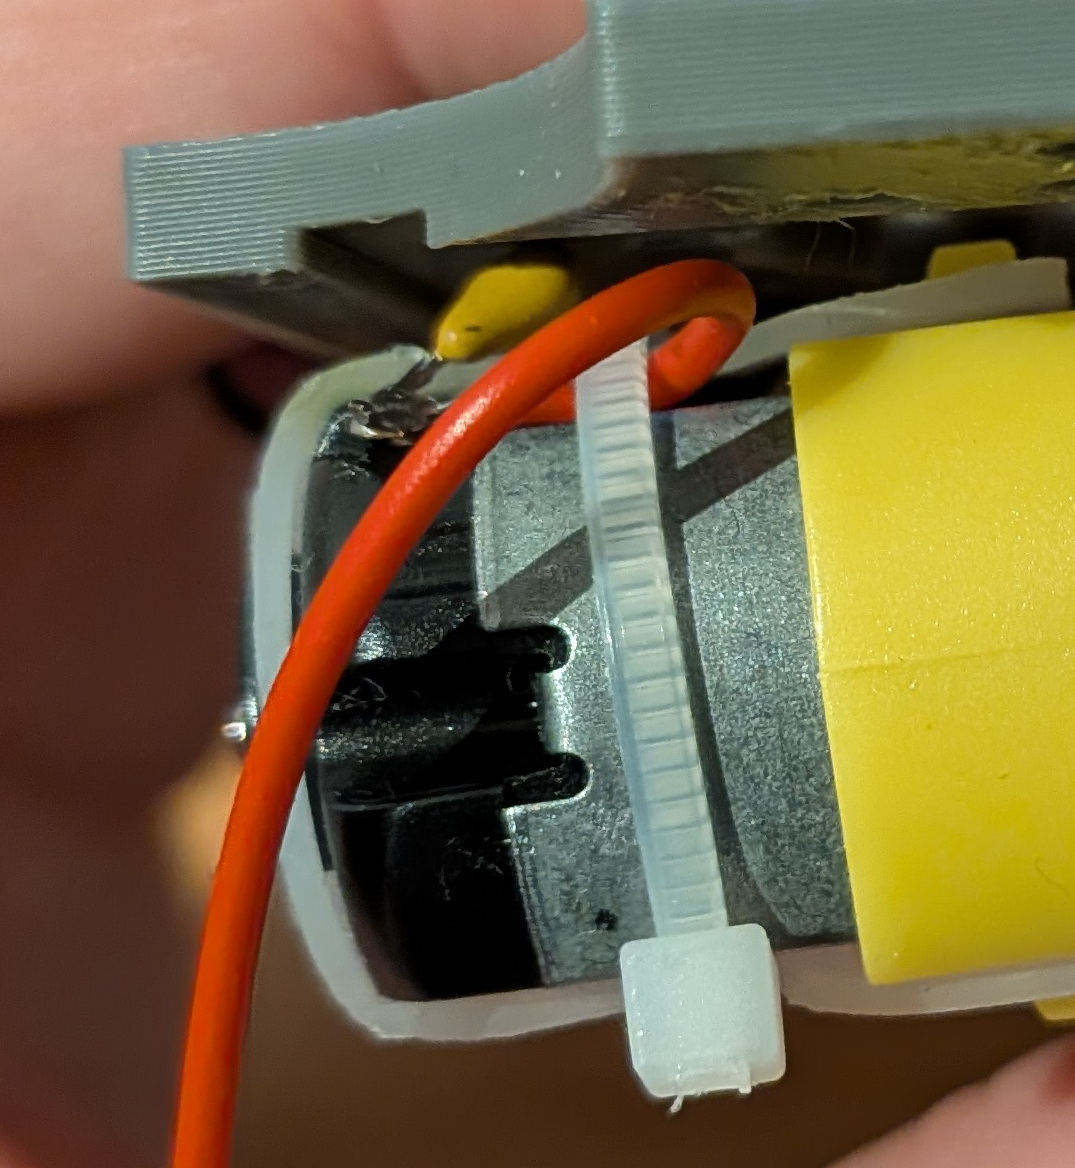
\includegraphics[scale=0.10]{montage_gereon/antrieb_montage/PXL_20260907_170730140.jpg}
\end{warnbox}


Nun wird jeder Motor mit den Streben auf den Seitenplatten montiert und außenseitig verschraubt. 

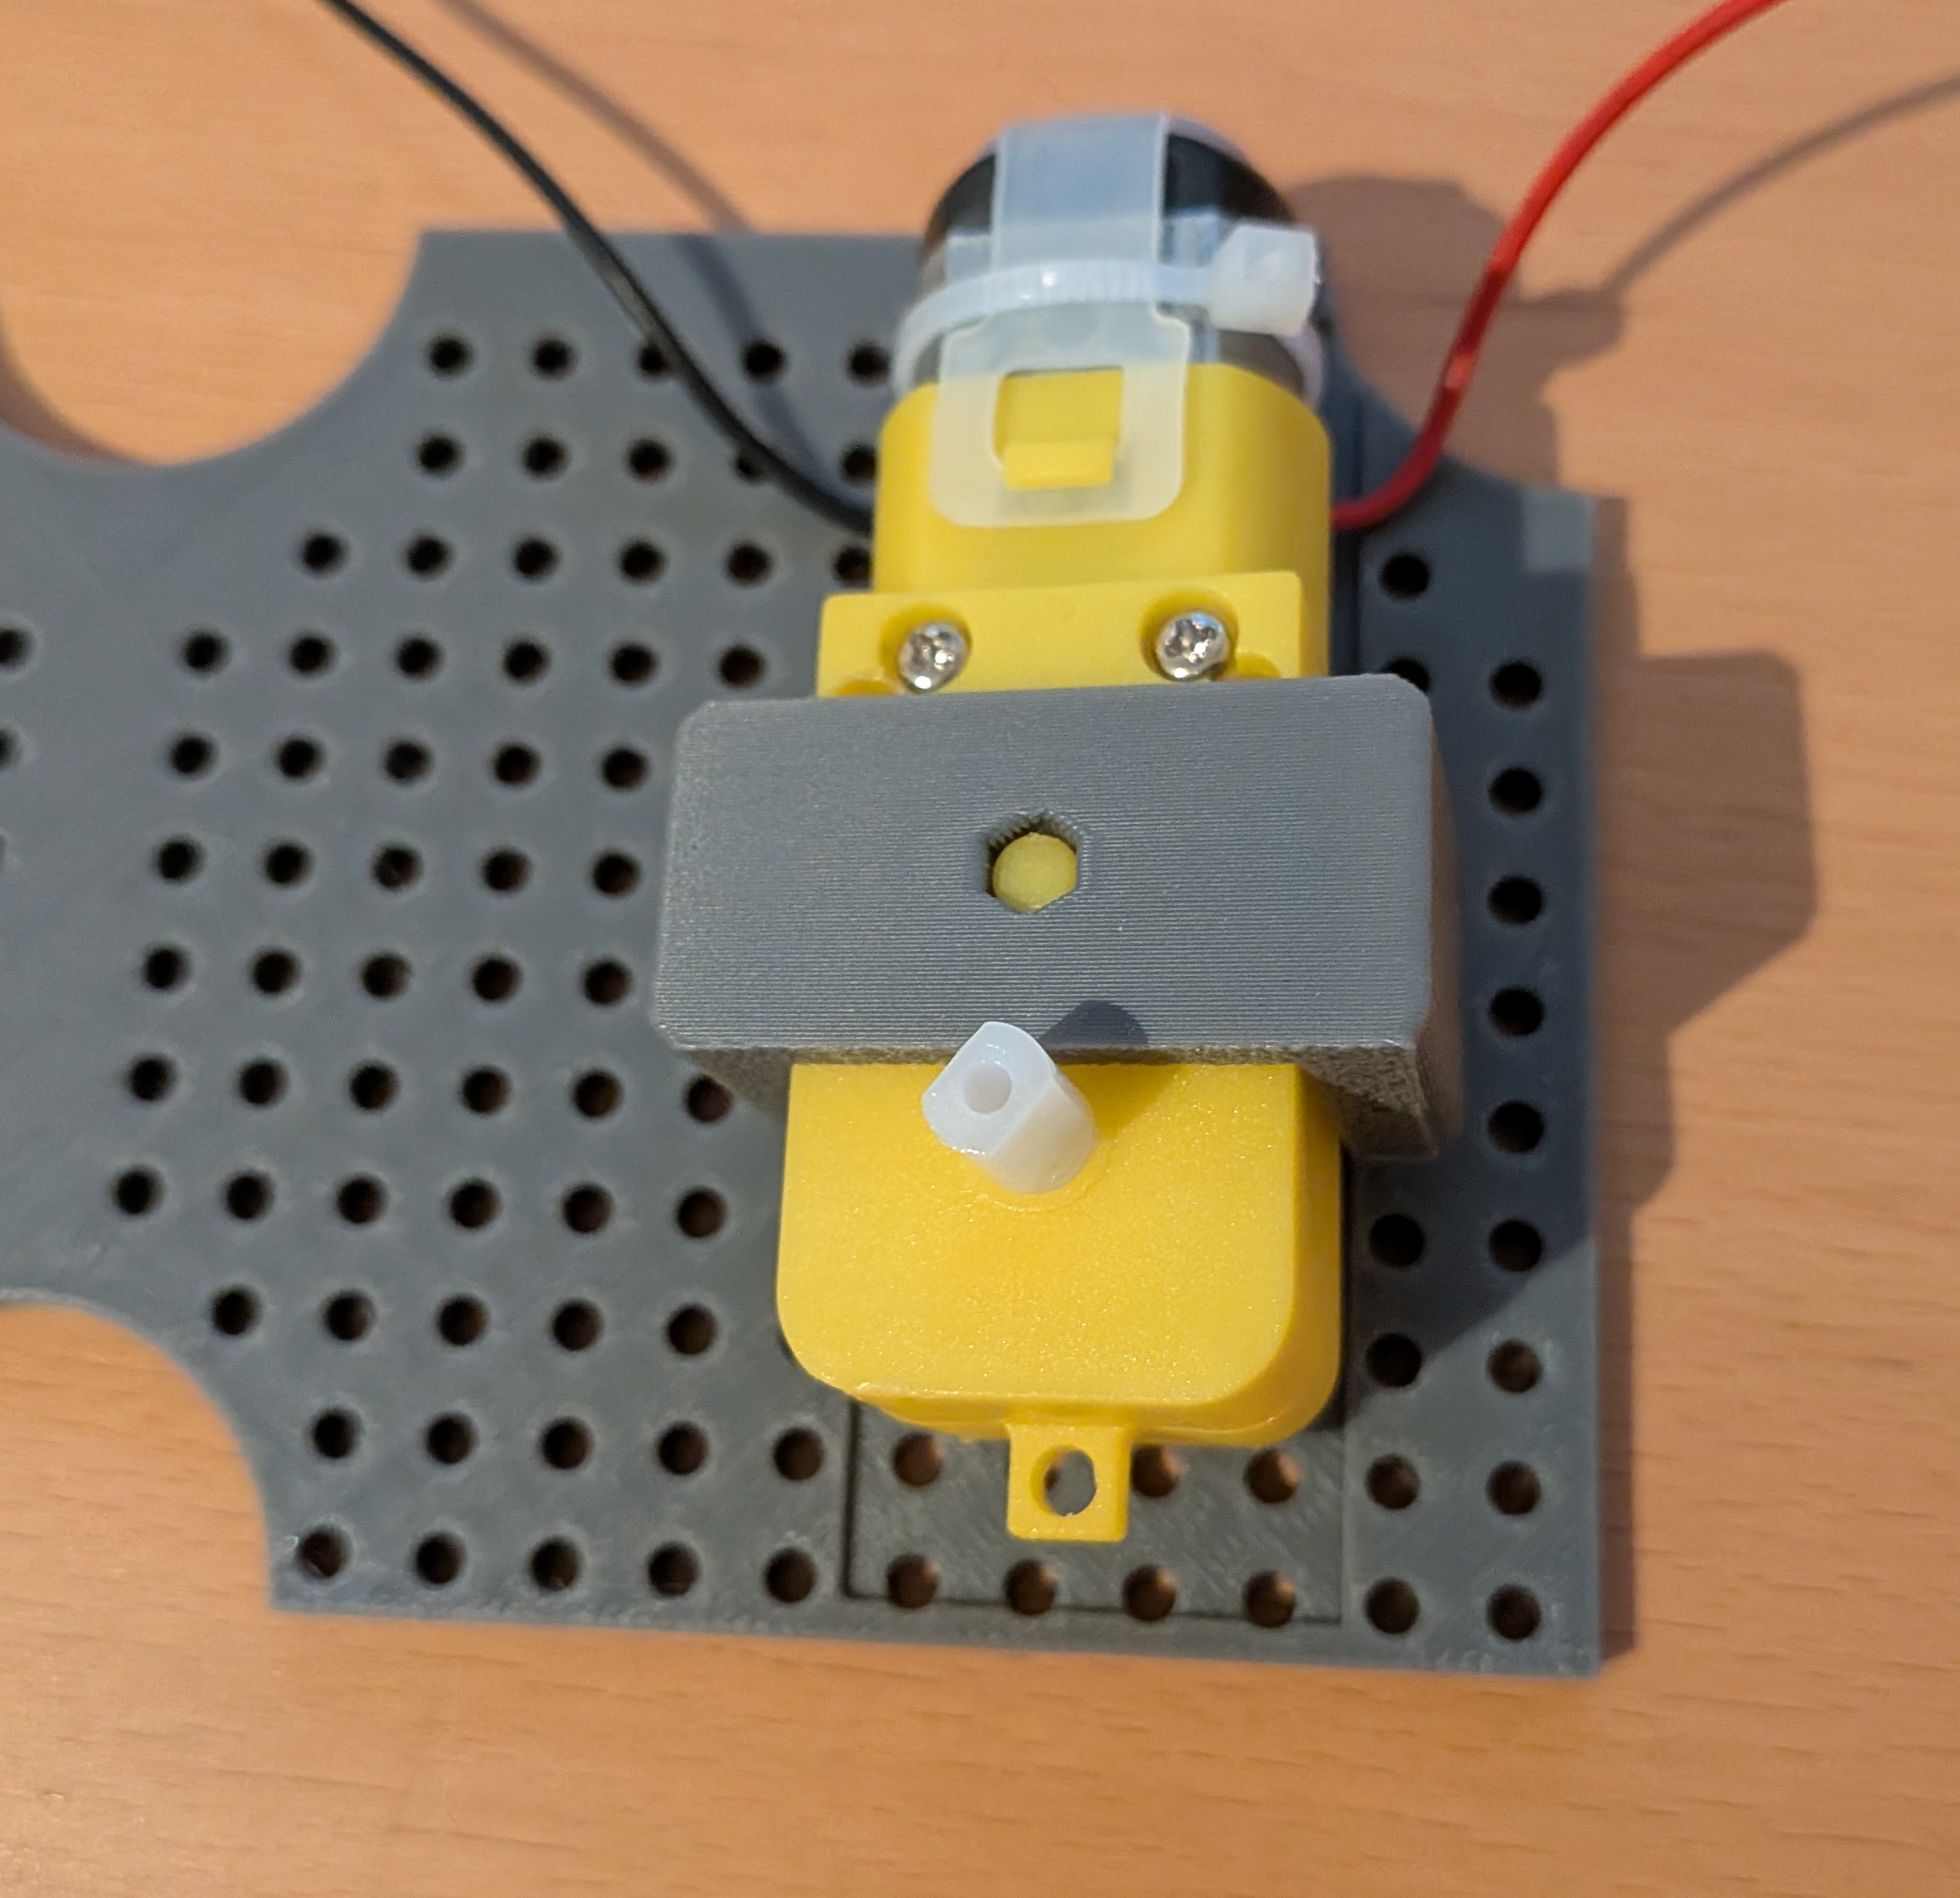
\includegraphics[scale=0.08]{montage_gereon/antrieb_montage/PXL_20260909_081306481.jpg}
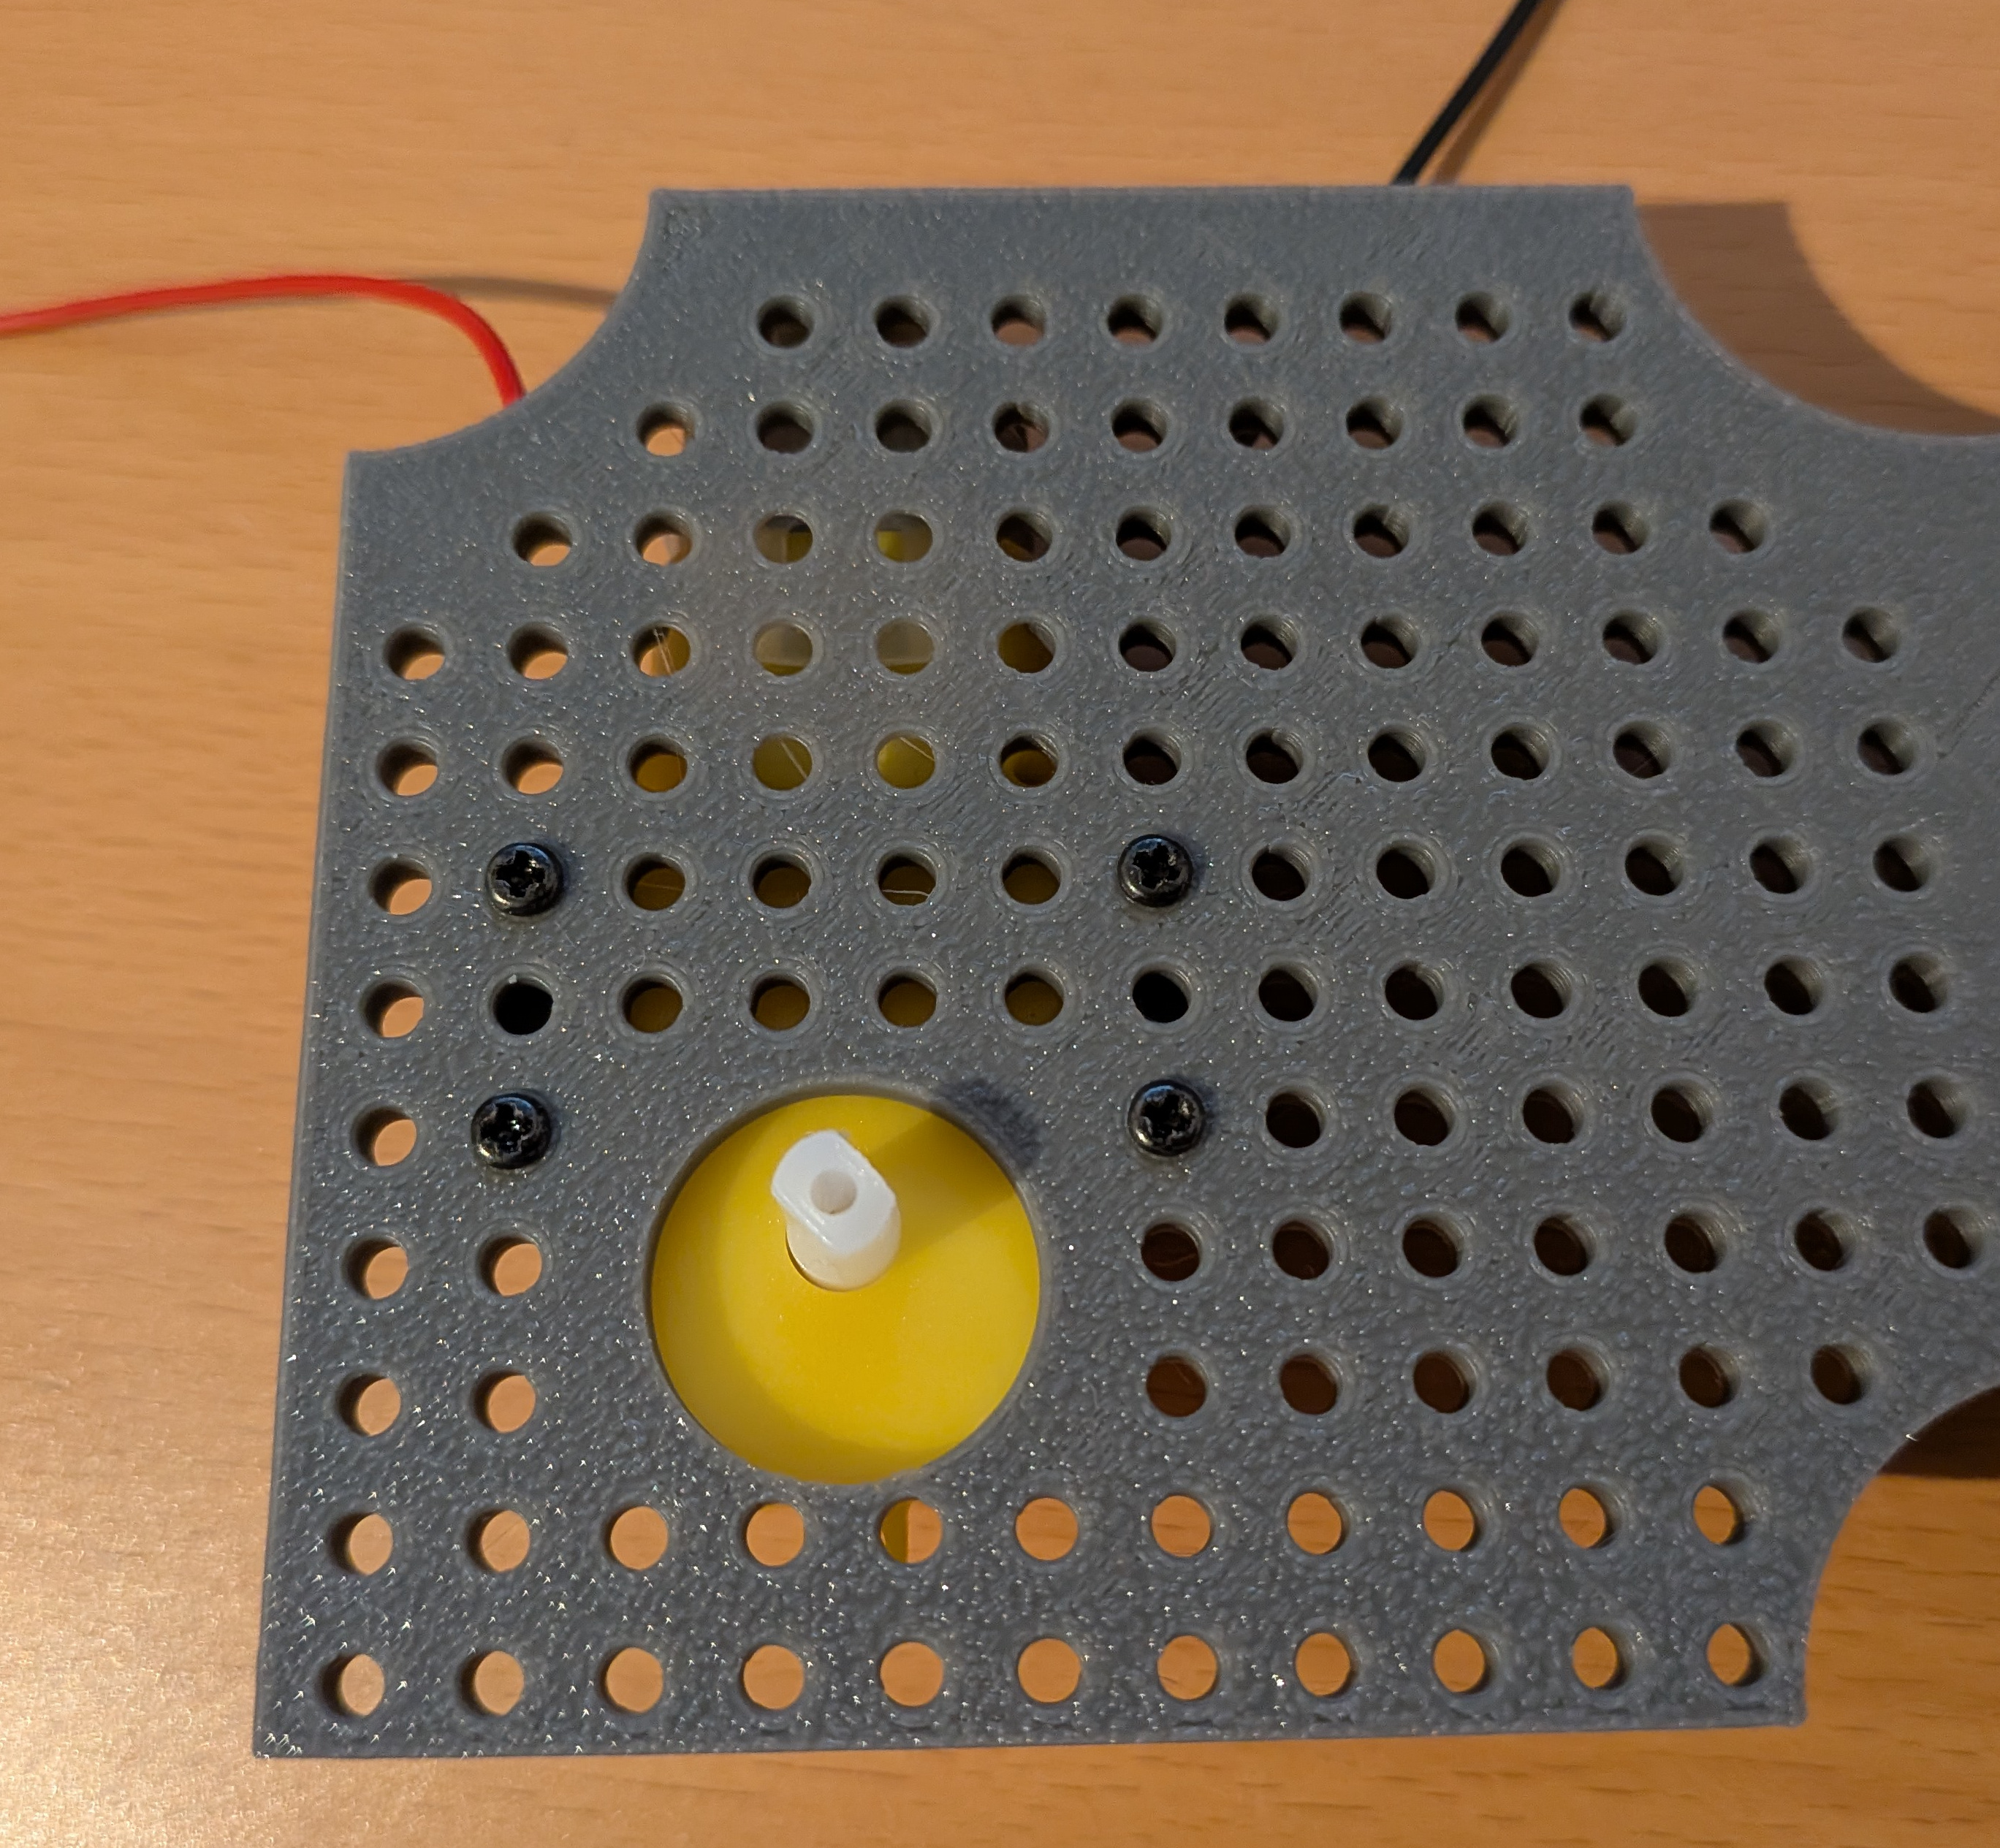
\includegraphics[scale=0.08]{montage_gereon/antrieb_montage/PXL_20260909_081443479.jpg}

So wird für beide Seitenwände verfahren. 

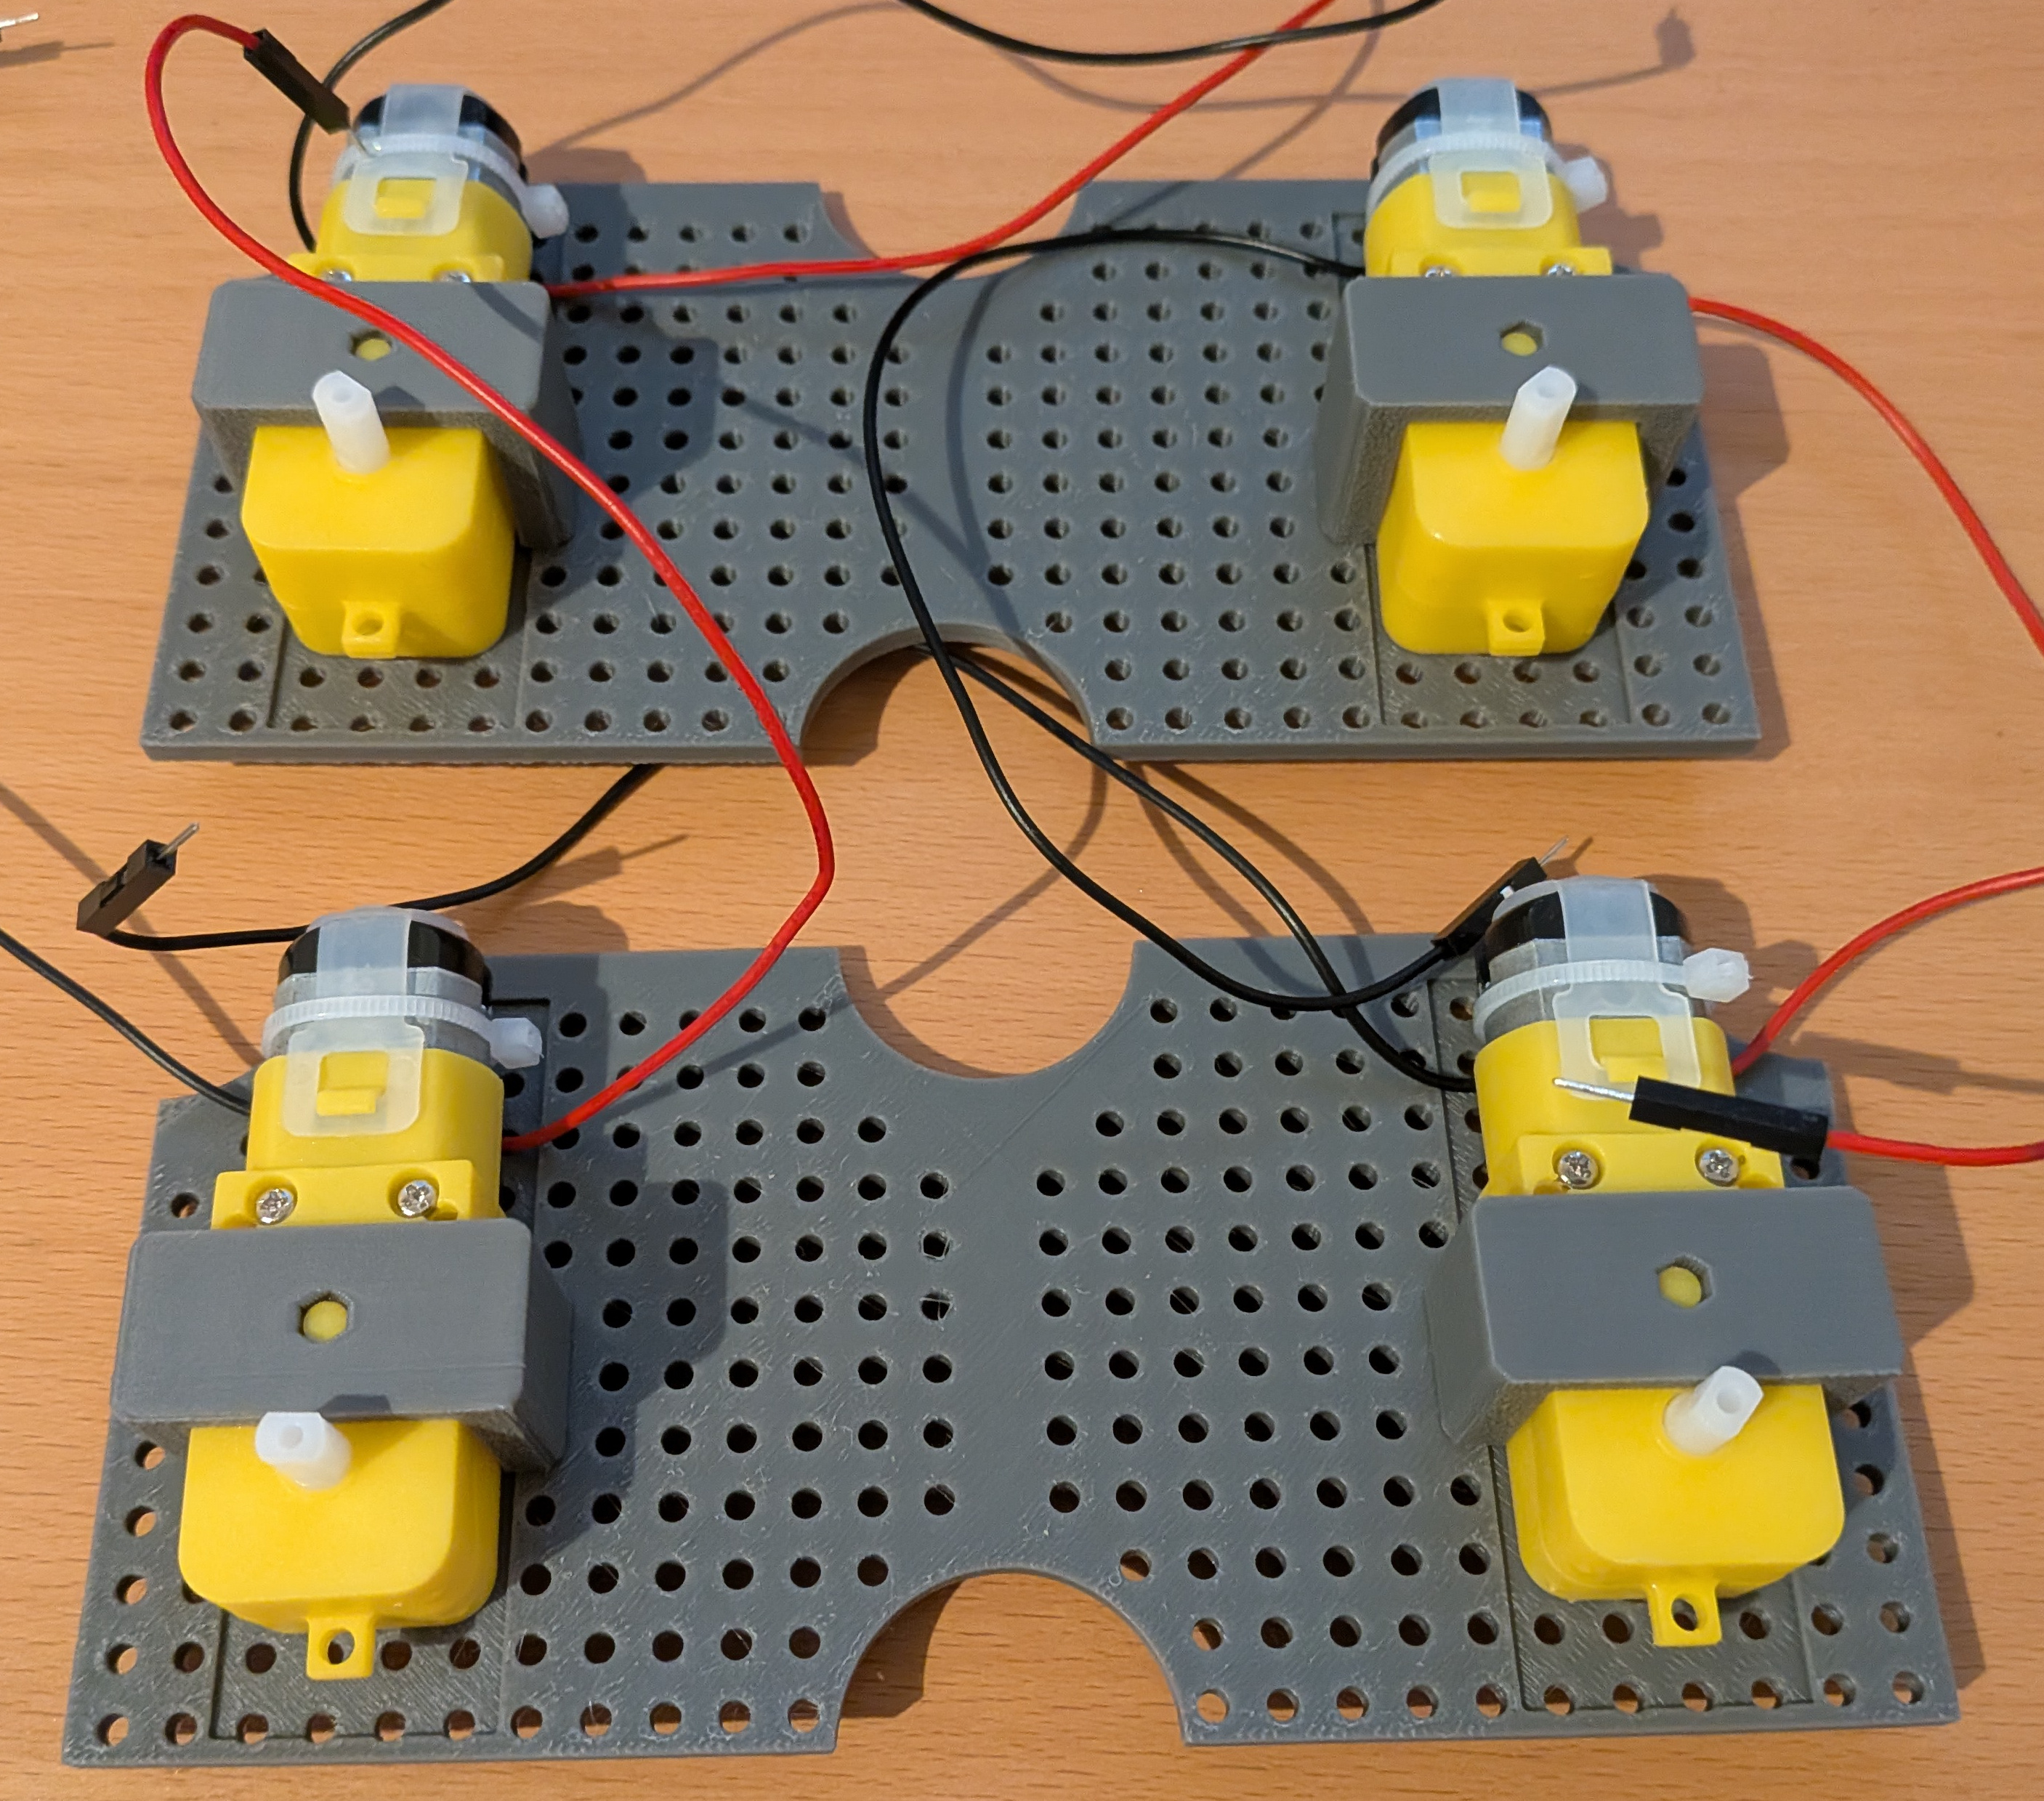
\includegraphics[scale=0.08]{montage_gereon/antrieb_montage/PXL_20260909_083634794.jpg}




\FloatBarrier
\subsection{Hauptplatine vorbereiten}

Die Hauptplatine fasst die zentralen Elektronikkomponenten zusammen und wird auf Lochraster verbunden. Die folgenden Hauptkomponenten werden somit zusammengefasst:

\begin{itemize}
\item DC/DC Step Up Converter Board
\item Microprocessorboard Raspberry Pi Pico 2
\item 2 mal TB6612FNG Motor Treiber Board
\item \textit{(Inertialsensor)}
\end{itemize}

Die Aktorik sowie die Sensorik wird über Pinheader verbunden. Es ergibt sich für eine Lochrastermontage damit der Aufbau gemäß der Abbildung \ref{fig:protoboard_mask_combined}. Im Einzelnen stellen diese folgende Ansichten dar:

\begin{figure}
    \centering
    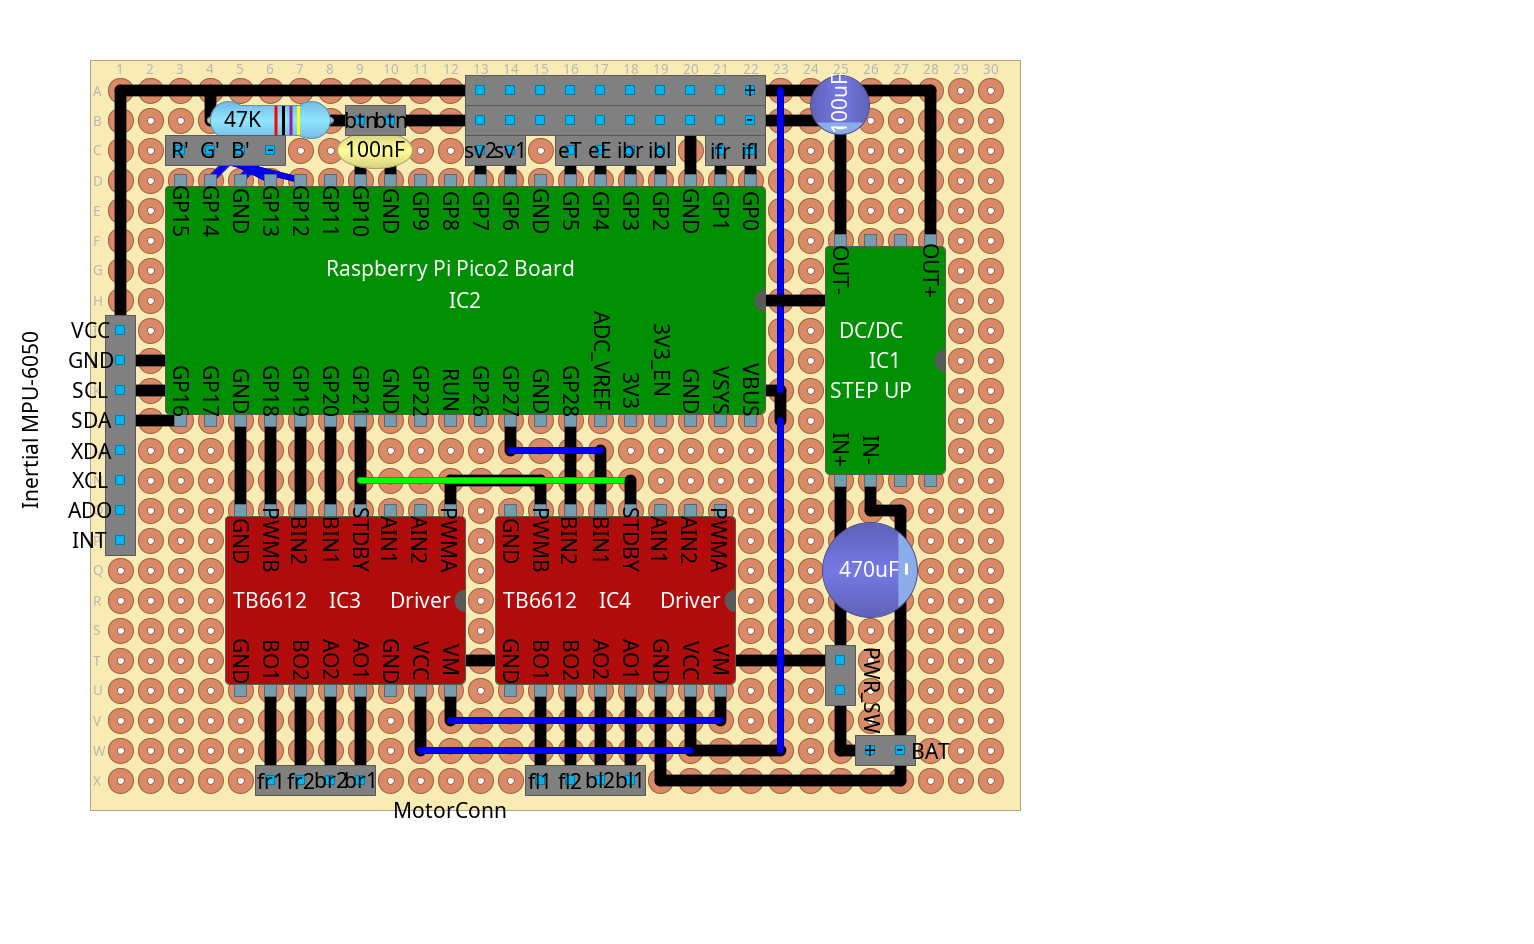
\includegraphics[width=0.8\linewidth]{protoboard_30x24_all.png}
    \caption{Kombinierte Ansicht Komponenten und Lötbrücken}
    \label{fig:protoboard_mask_combined}
\end{figure}

Das Lochraster Layout wurde mittels der Software DIYLC \footnote{\url{https://github.com/bancika/diy-layout-creator}} erstellt und die Source Dateien finden sich im Github Repository \footnote{\url{https://github.com/Project-CoasterBot/coasterbot/blob/main/M4_Test-und-Validierung/aufbauanleitung/protoboard.diy}}. 

\FloatBarrier

Die Platine wird nun bestückt und verdrahtet:

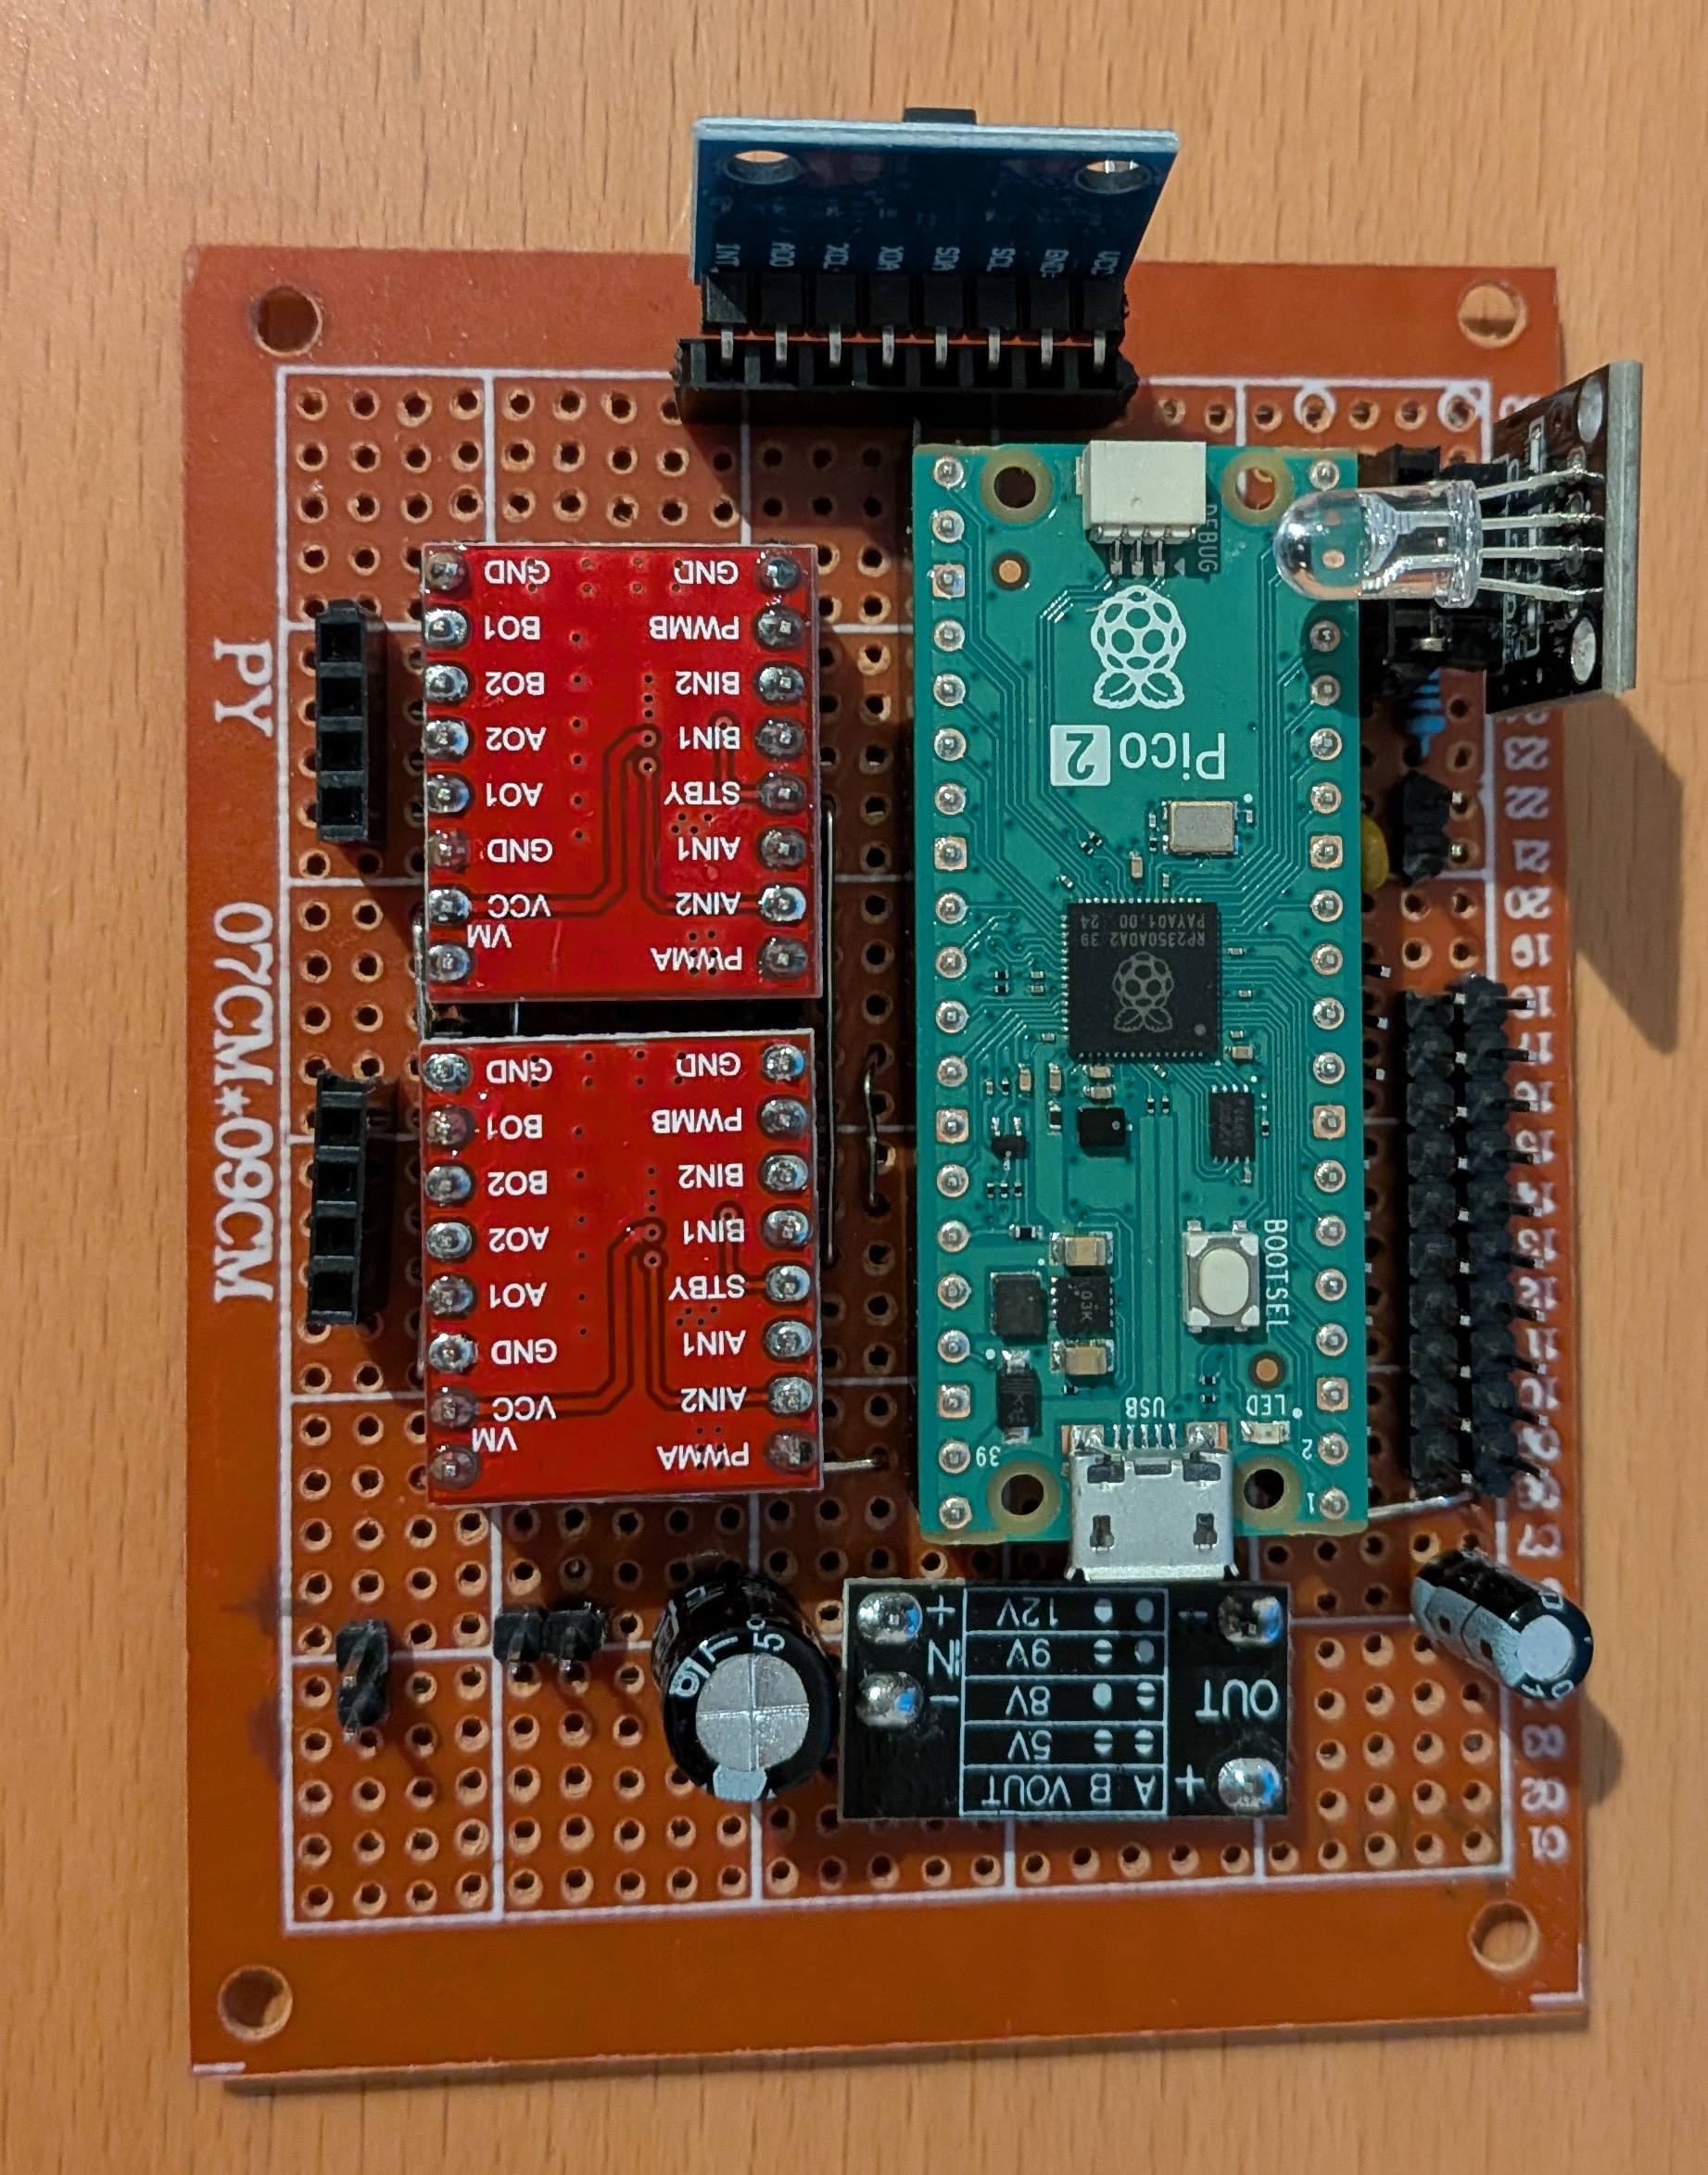
\includegraphics[scale=0.08]{montage_gereon/platine/PXL_20260912_172856294.jpg}
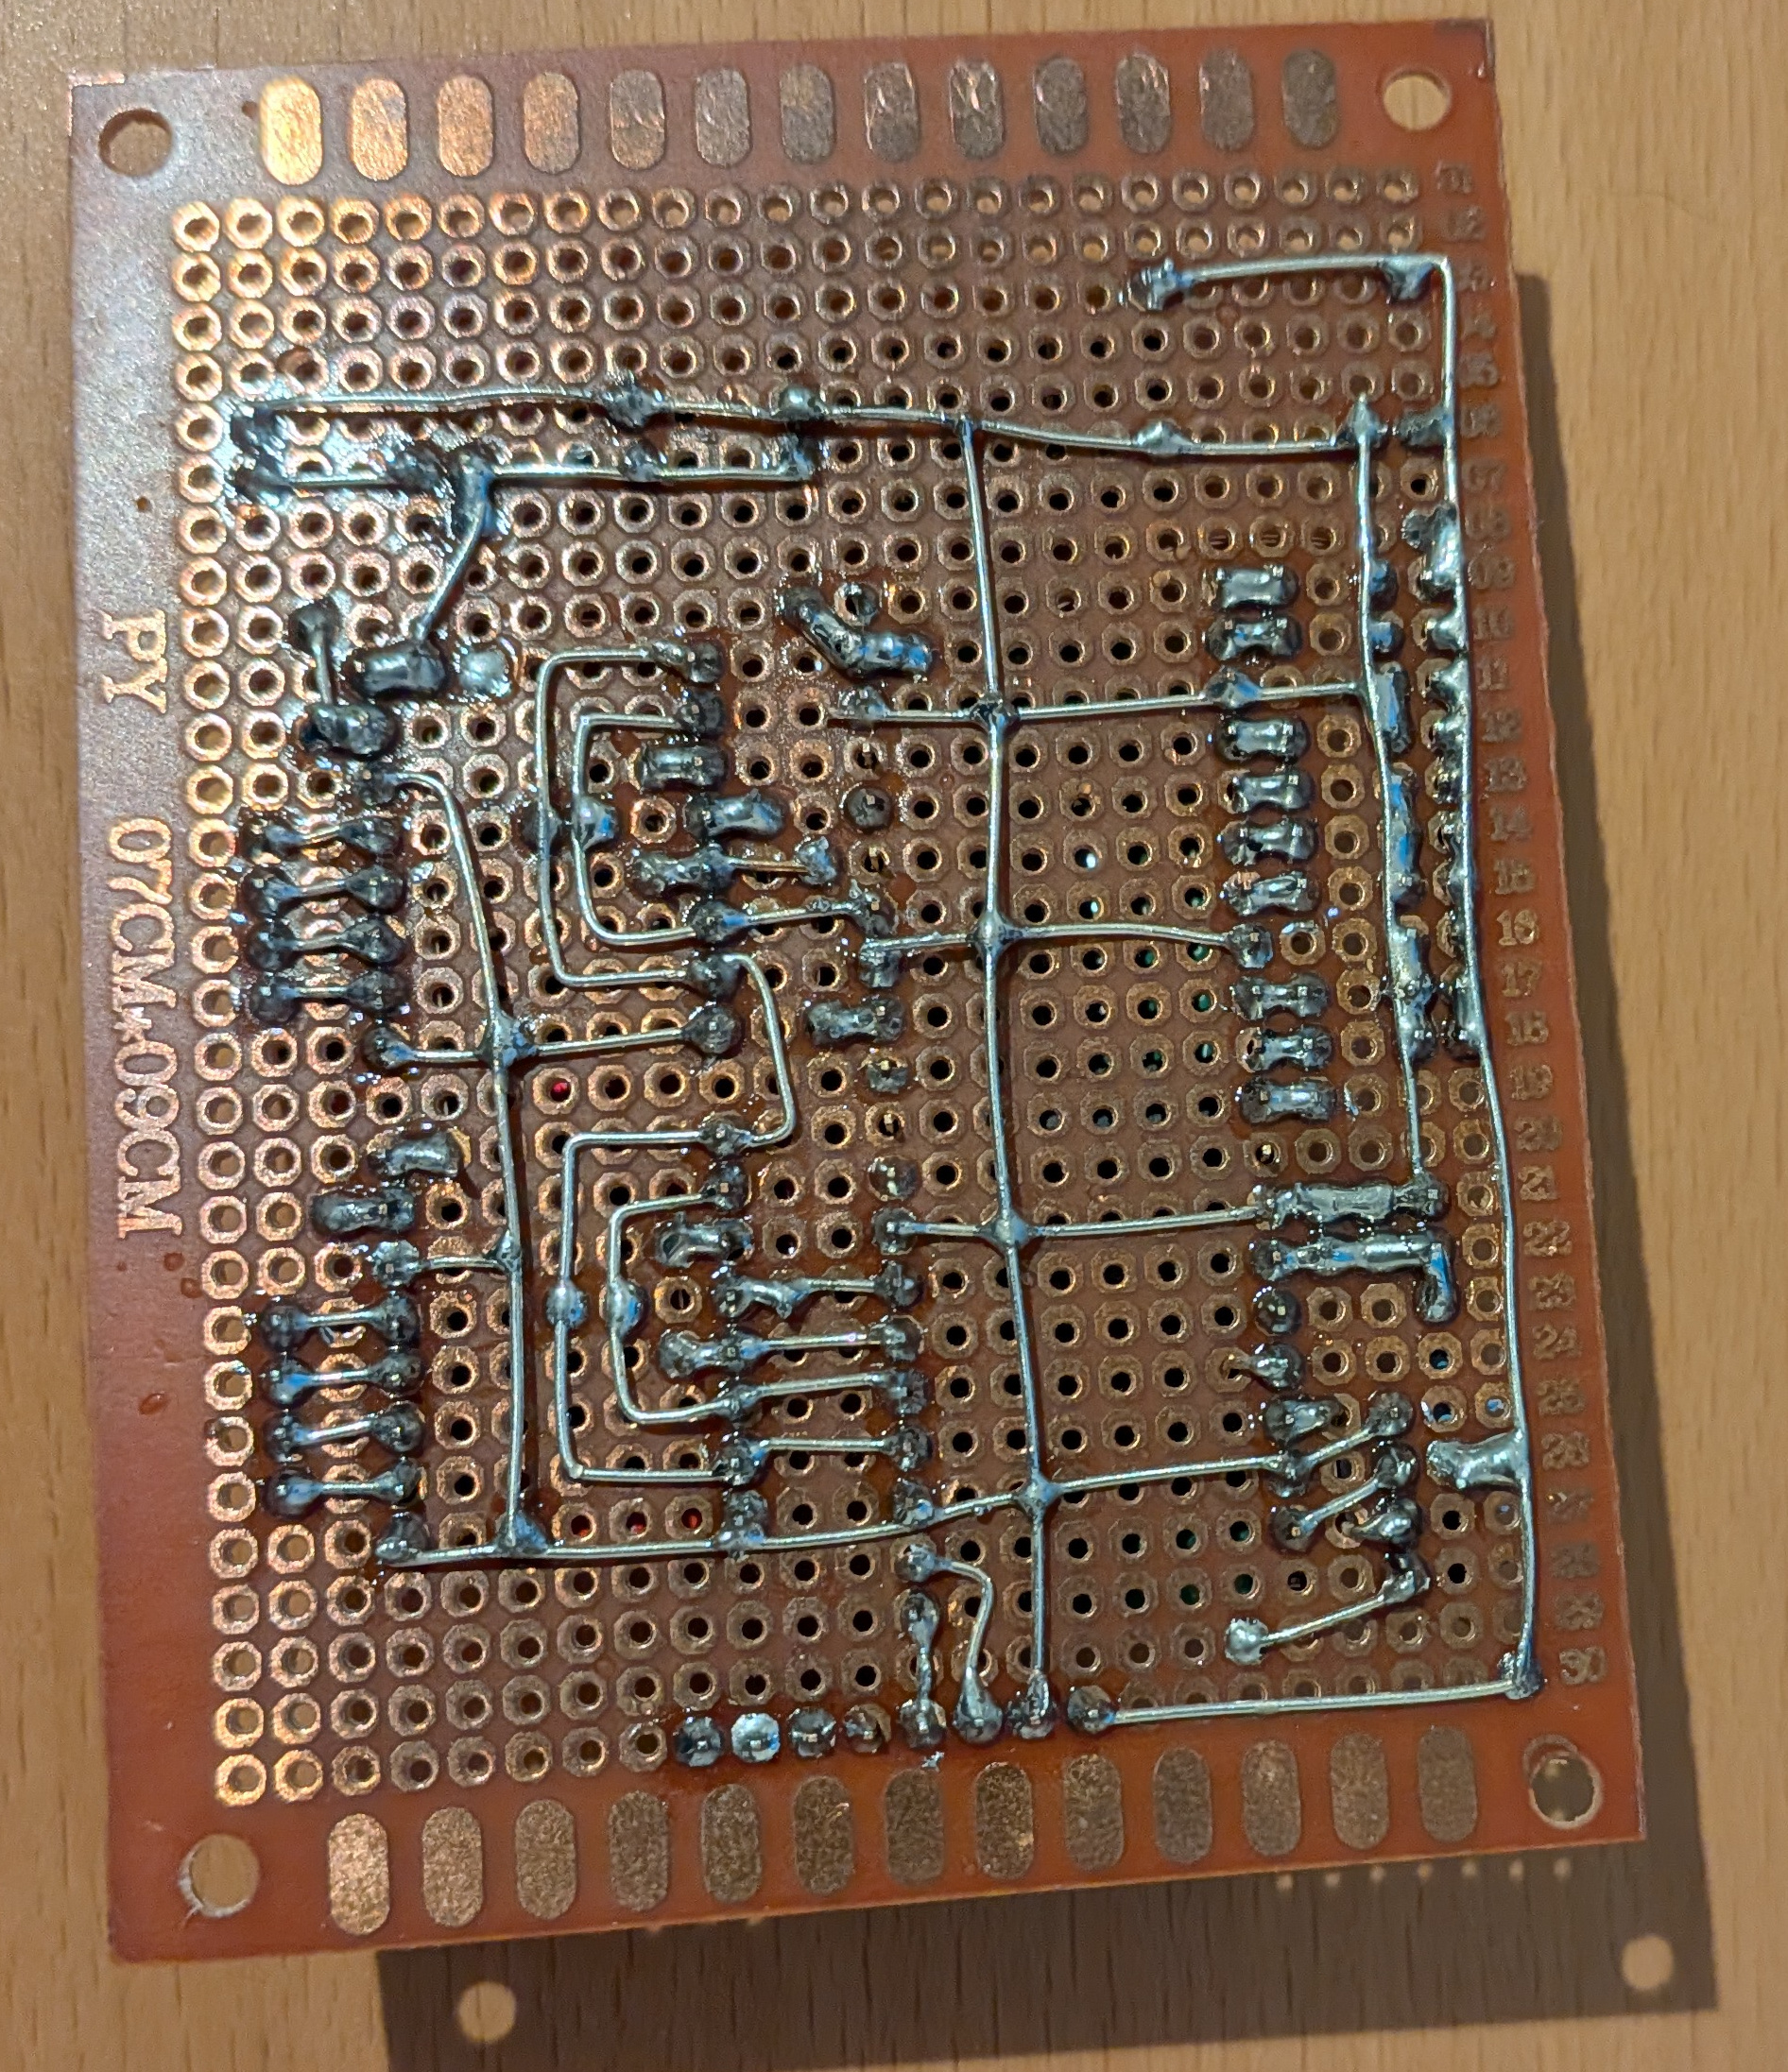
\includegraphics[scale=0.08]{montage_gereon/platine/PXL_20260912_172906337.jpg}

Anschließend wird diese auf der hinteren Platte zusammen mit dem Akkuhalter montiert. Dabei ist zu beachten, dass der Batterieanschluss (+- BAT) der Platine an der Seite des Batterieträgers montiert wird. 

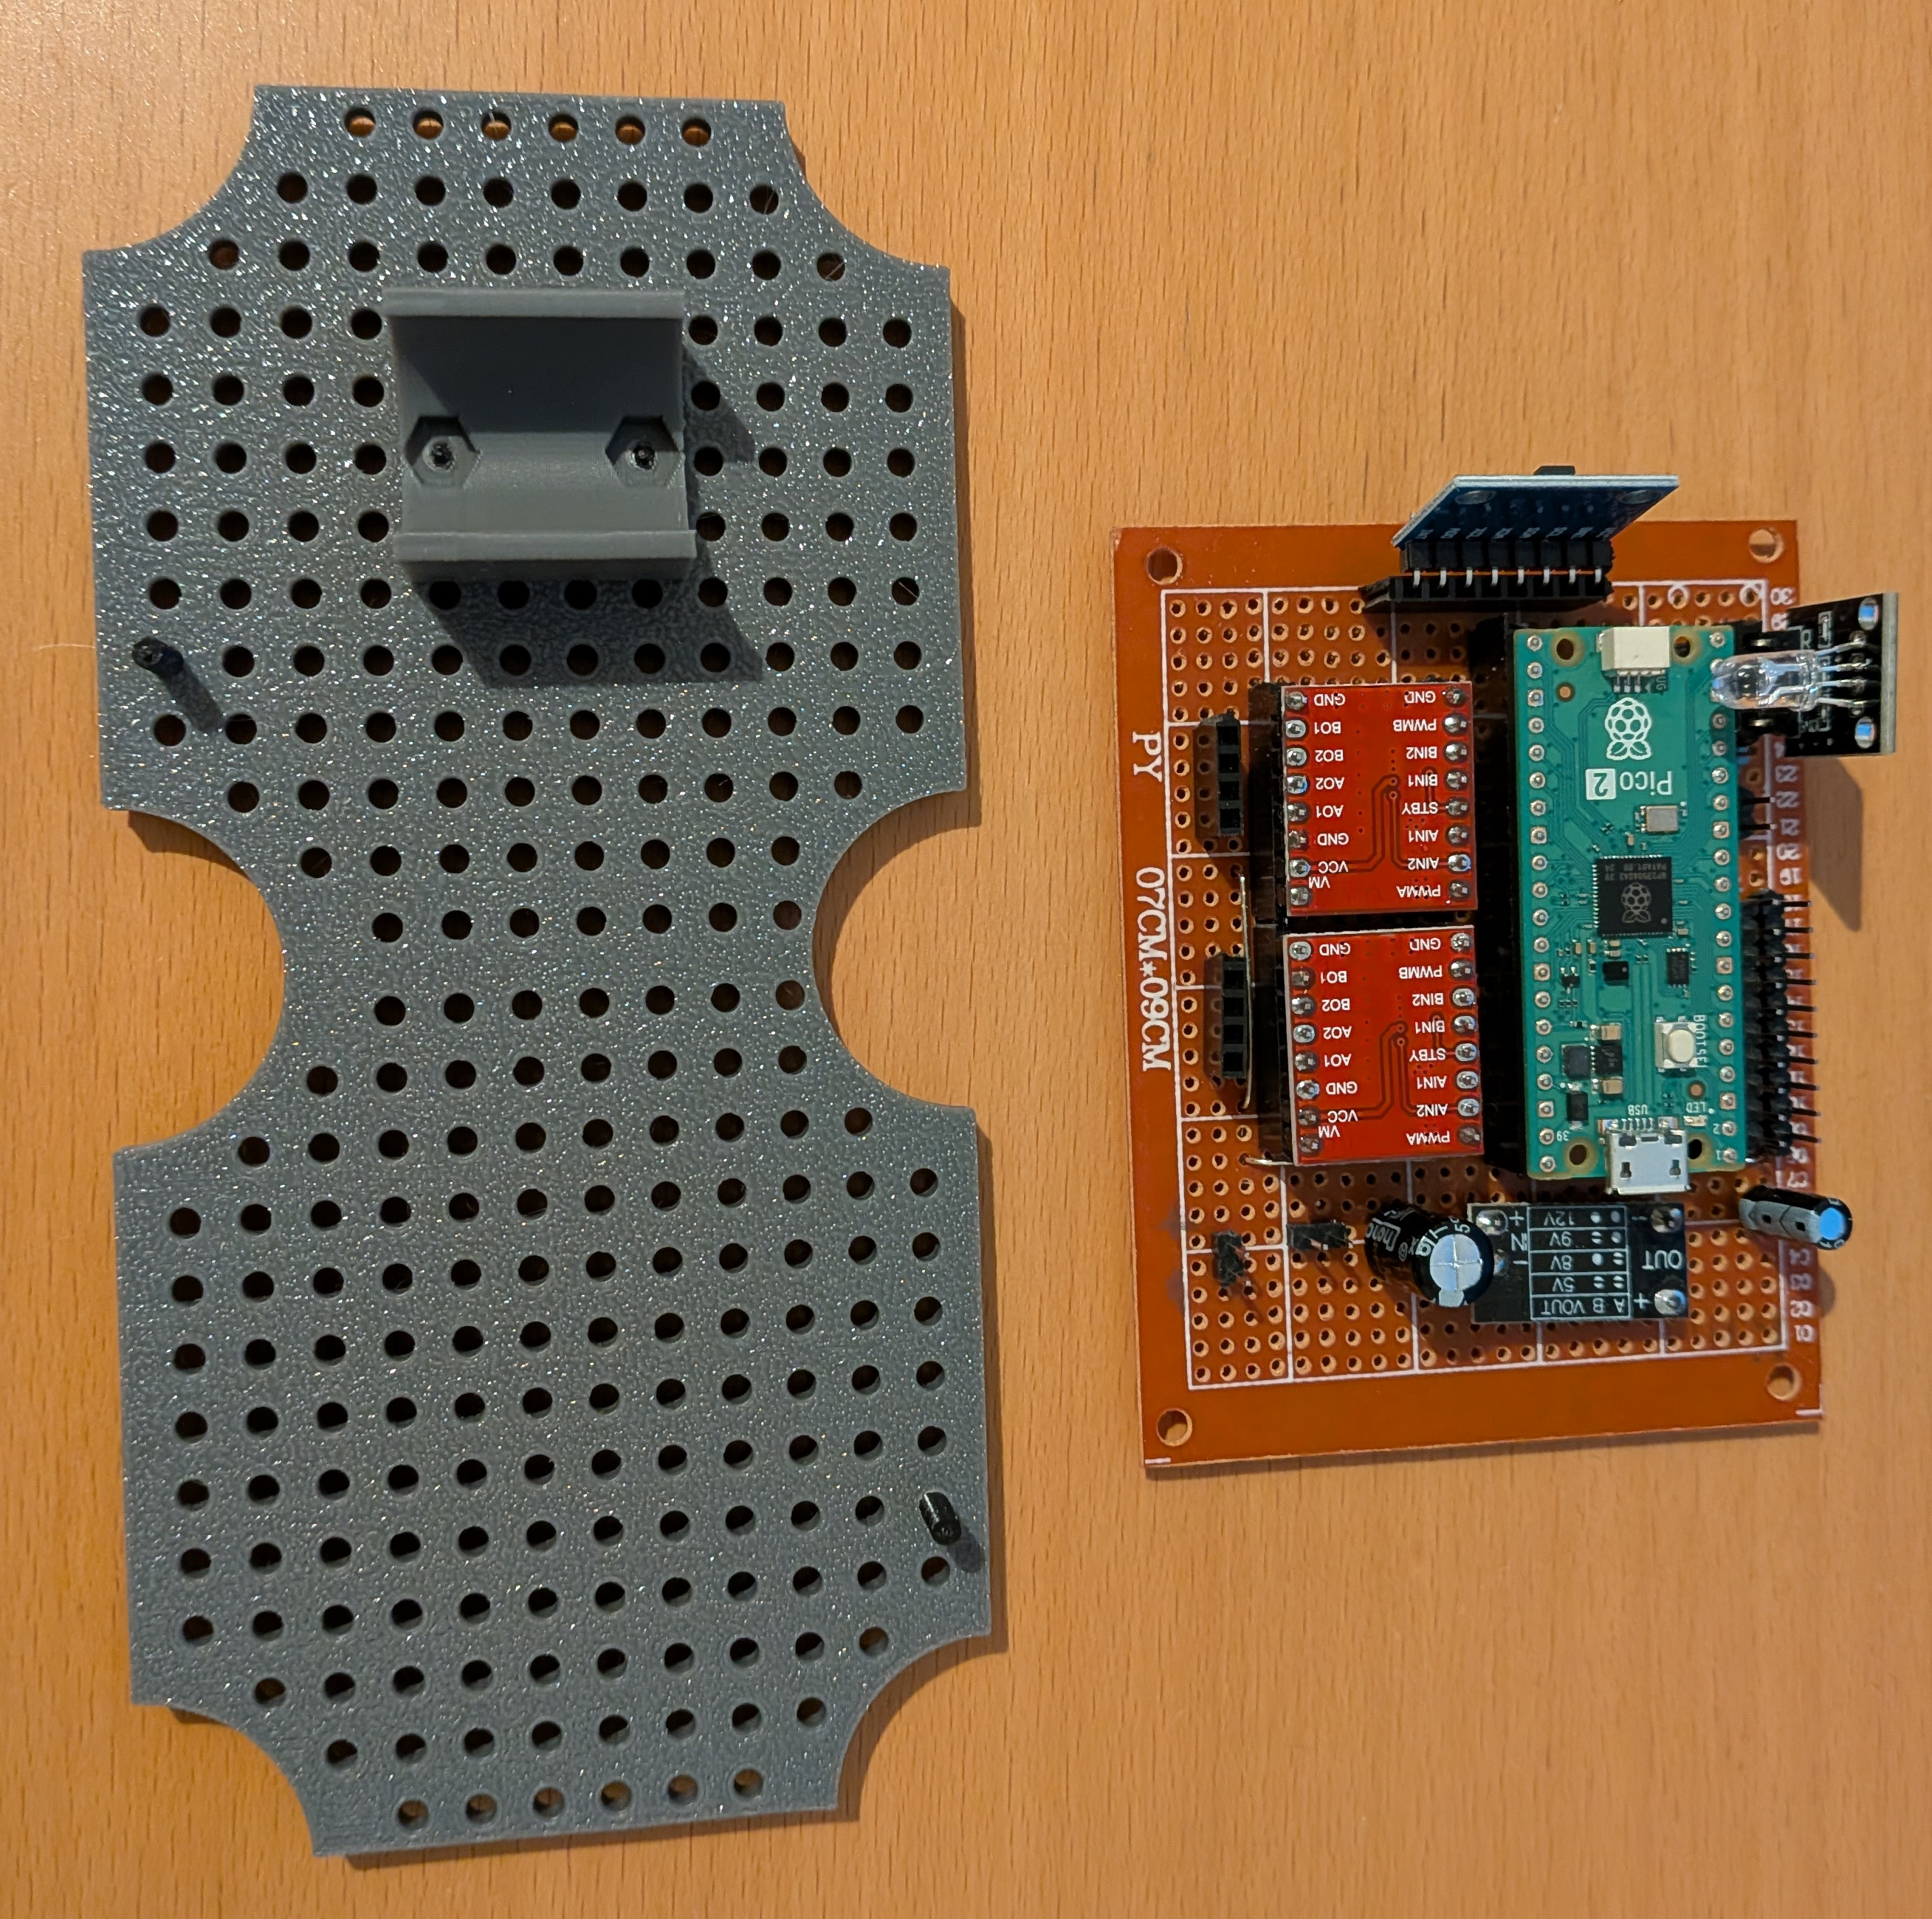
\includegraphics[scale=0.08]{montage_gereon/platine/PXL_20260912_173108019.jpg}




\subsection{Programmierung des Microcontrollers}

\begin{warnbox}
Während der Microcontroller über den USB Port verbunden ist muss die Spannungsversorgung des Coasterbots getrennt werden. Falls der Akku montiert ist muss dieser entfernt werden, andernfalls droht eine Beschädigung des Microcontrollers. 
\end{warnbox}


Das Microcontroller Board über die boardeigene Micro USB Buchse mit dem Host-PC verbunden.

Die Firmware befindet sich im Github Repository des Projekts\footnote{\url{https://github.com/Project-CoasterBot/coasterbot/tree/main/src}} und kann von dort bezogen werden.

Die Software wird in der Build Umgebung mit den folgenden Befehlen kompiliert und an den Microcontroller übertragen. 

\begin{verbatim}
$ cd PROJDIR
$ cmake .
$ make
$ ... TODO
\end{verbatim}

Anschließend kann das USB Kabel wieder entfernt werden. 


\subsection{Sensorik und Steuerung Montage}

Nun werden die Infrarot Module an Front und Rückplatte montiert. Dabei ist auf einen korrekten Abstand sowohl zur Unterseite als auch nach außen zu achten. 

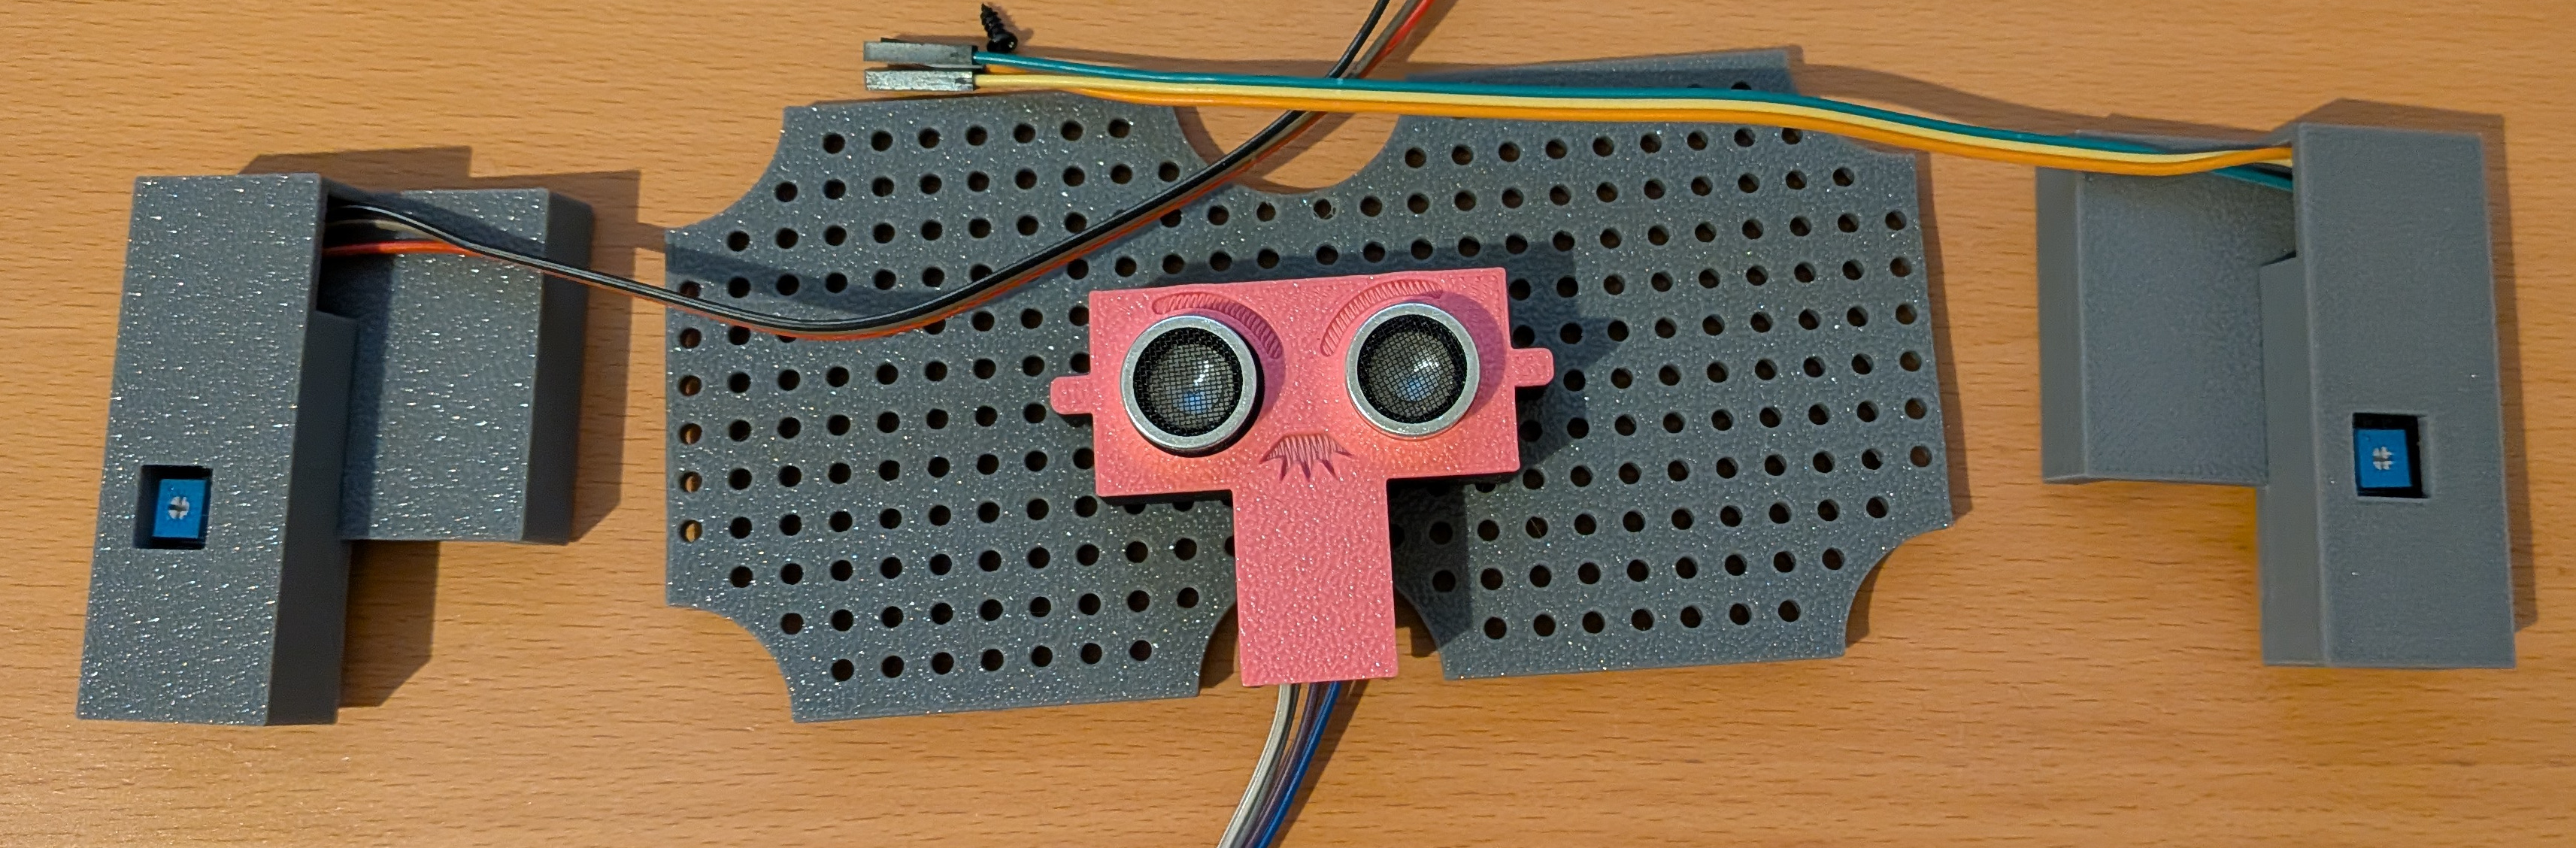
\includegraphics[scale=0.06]{montage_gereon/gesamt_montage/PXL_20260912_200037860.jpg}
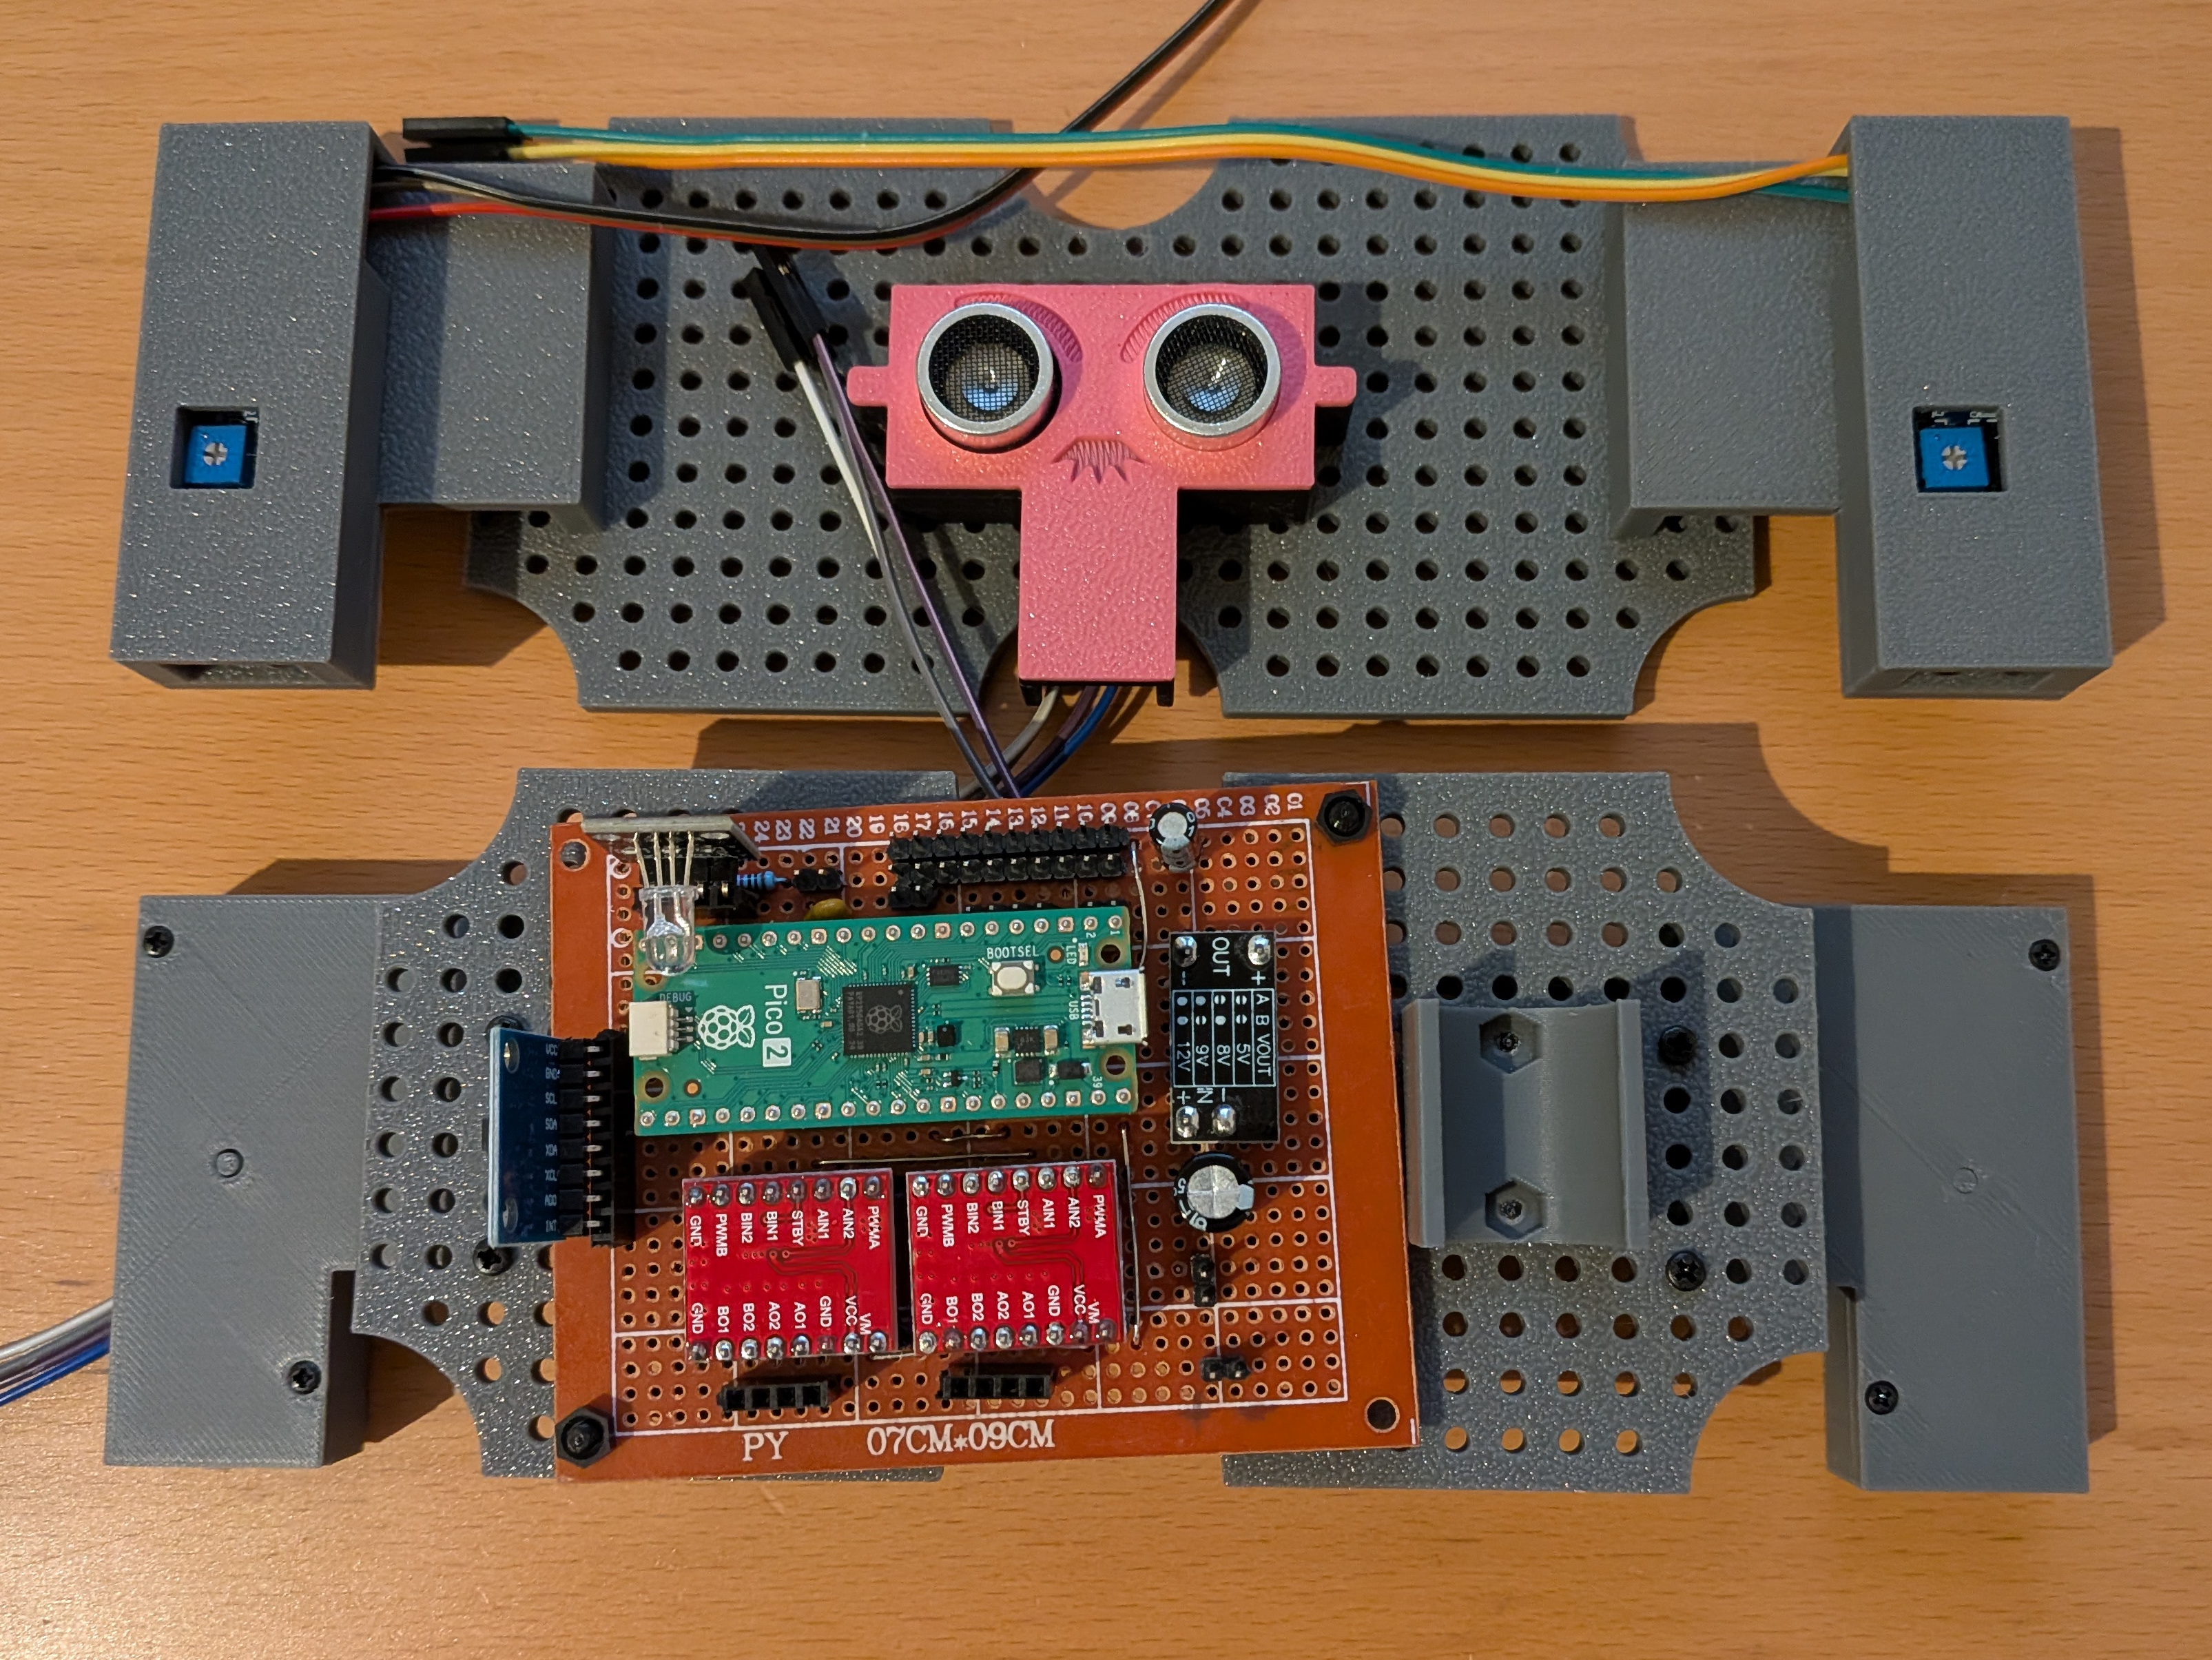
\includegraphics[scale=0.06]{montage_gereon/gesamt_montage/PXL_20260912_200913185.jpg}

Die Vorderplatte kann nun in das Chassis eingesetzt werden. Dabei ist darauf zu achten, dass die Verbinder nach innen positioniert werden. 

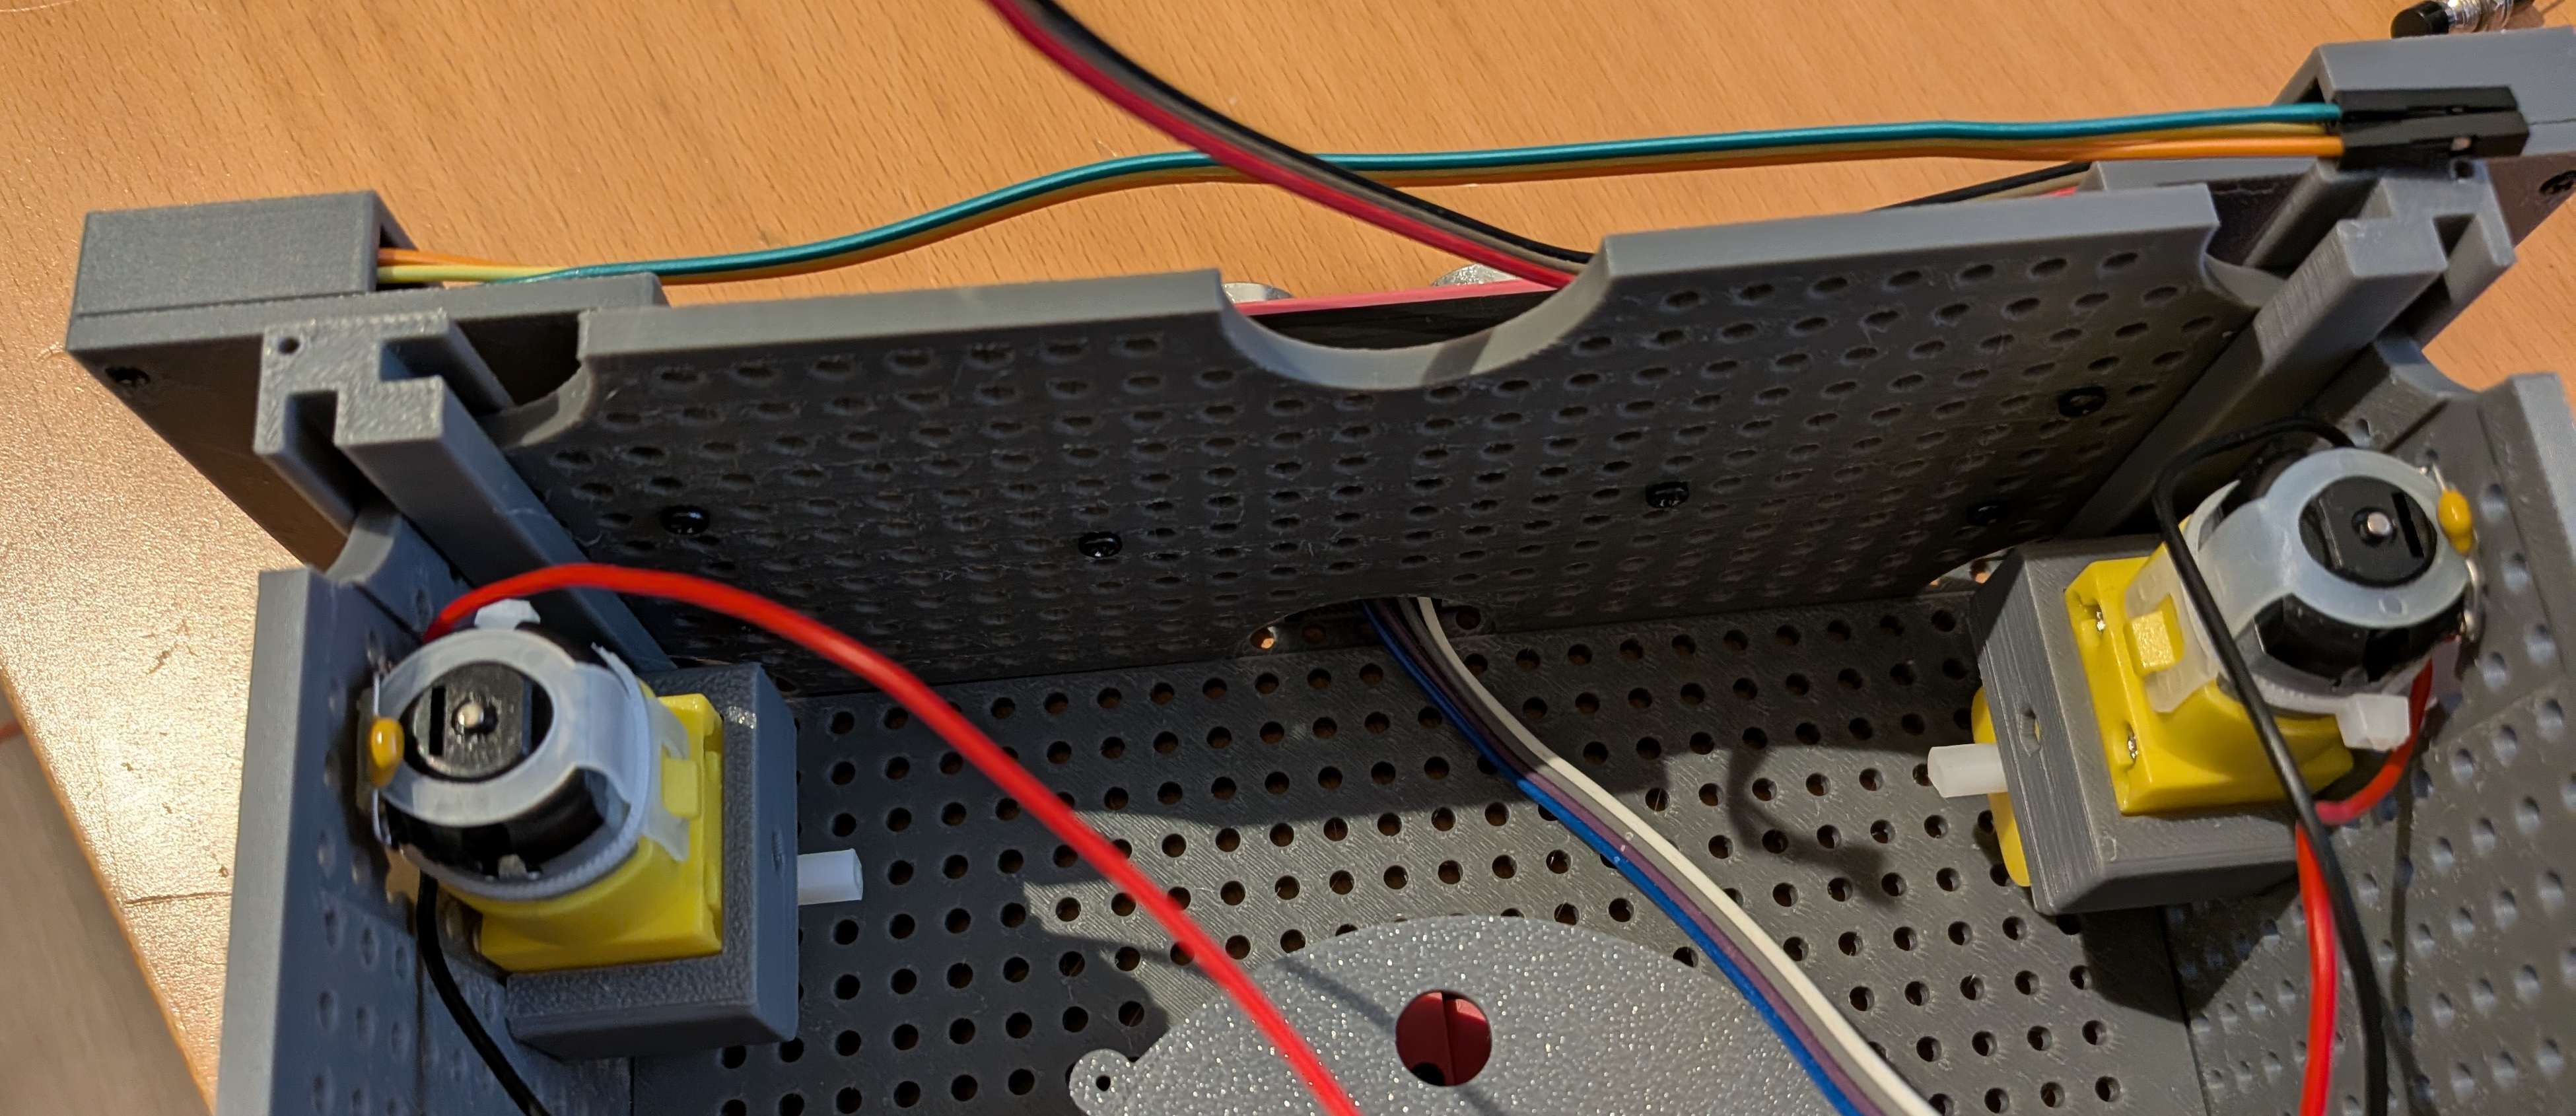
\includegraphics[scale=0.08]{montage_gereon/gesamt_montage/PXL_20260912_200946614.jpg}
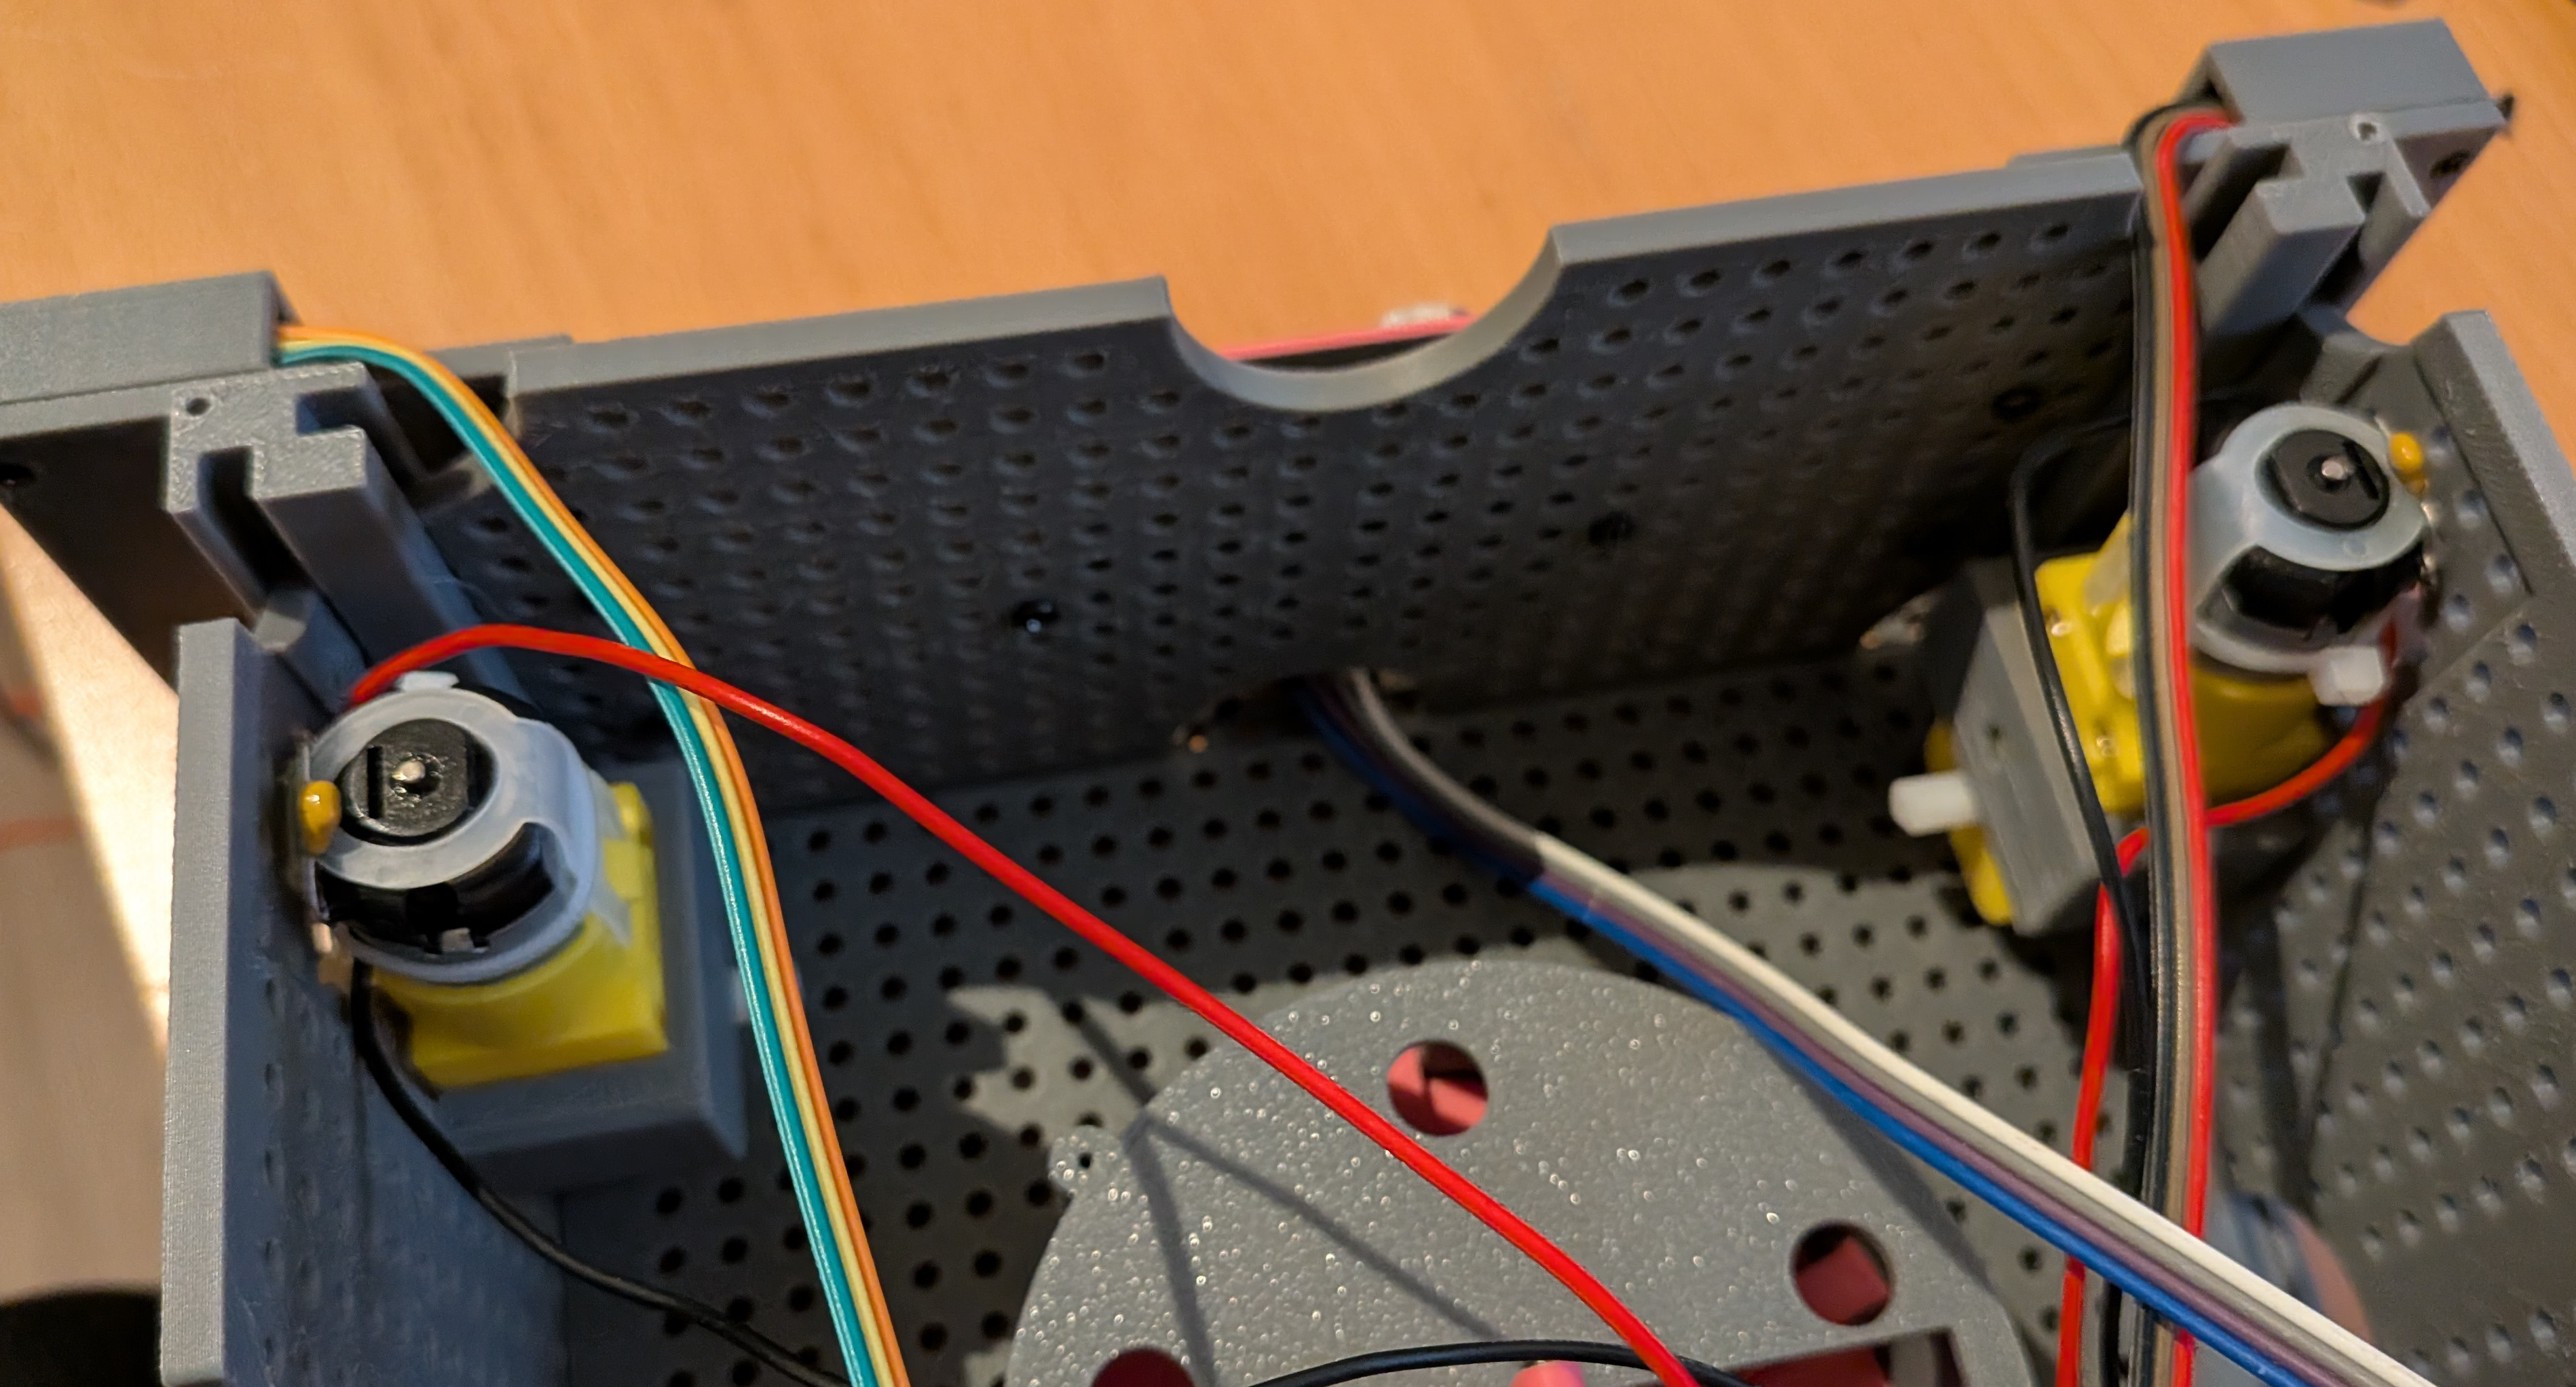
\includegraphics[scale=0.08]{montage_gereon/gesamt_montage/PXL_20260912_201010425.jpg}



\subsection{Verbinden der Aktorik und Sensorik mit Hauptplatine}



Die Aktorik und Sensorik Module werden zunächst entsprechend dem Schaltplan bzw. Lochrasterplan mit den korrekten Pin Headern verbunden. Dabei ist auf eine korrekte Kabelführung zu achten, sodass die Aktorik nicht durch die Verbinder gestört wird. Wir beginnen zunächst mit den Motoren und der Batterie, da diese an der Unterseite liegen und nach einfügen der Rückplatte schlecht erreichbar sind. Bei den vorderen Verbindern ist zu beachten, dass aufgrund der Größe des Gehäuses die Verbinder möglicherweise zu kurz sind, dies wurde hier für die Antriebsmotoren links und rechts durchgeführt, sowie im zweiten Bild Akku und Hauptschalter montiert:

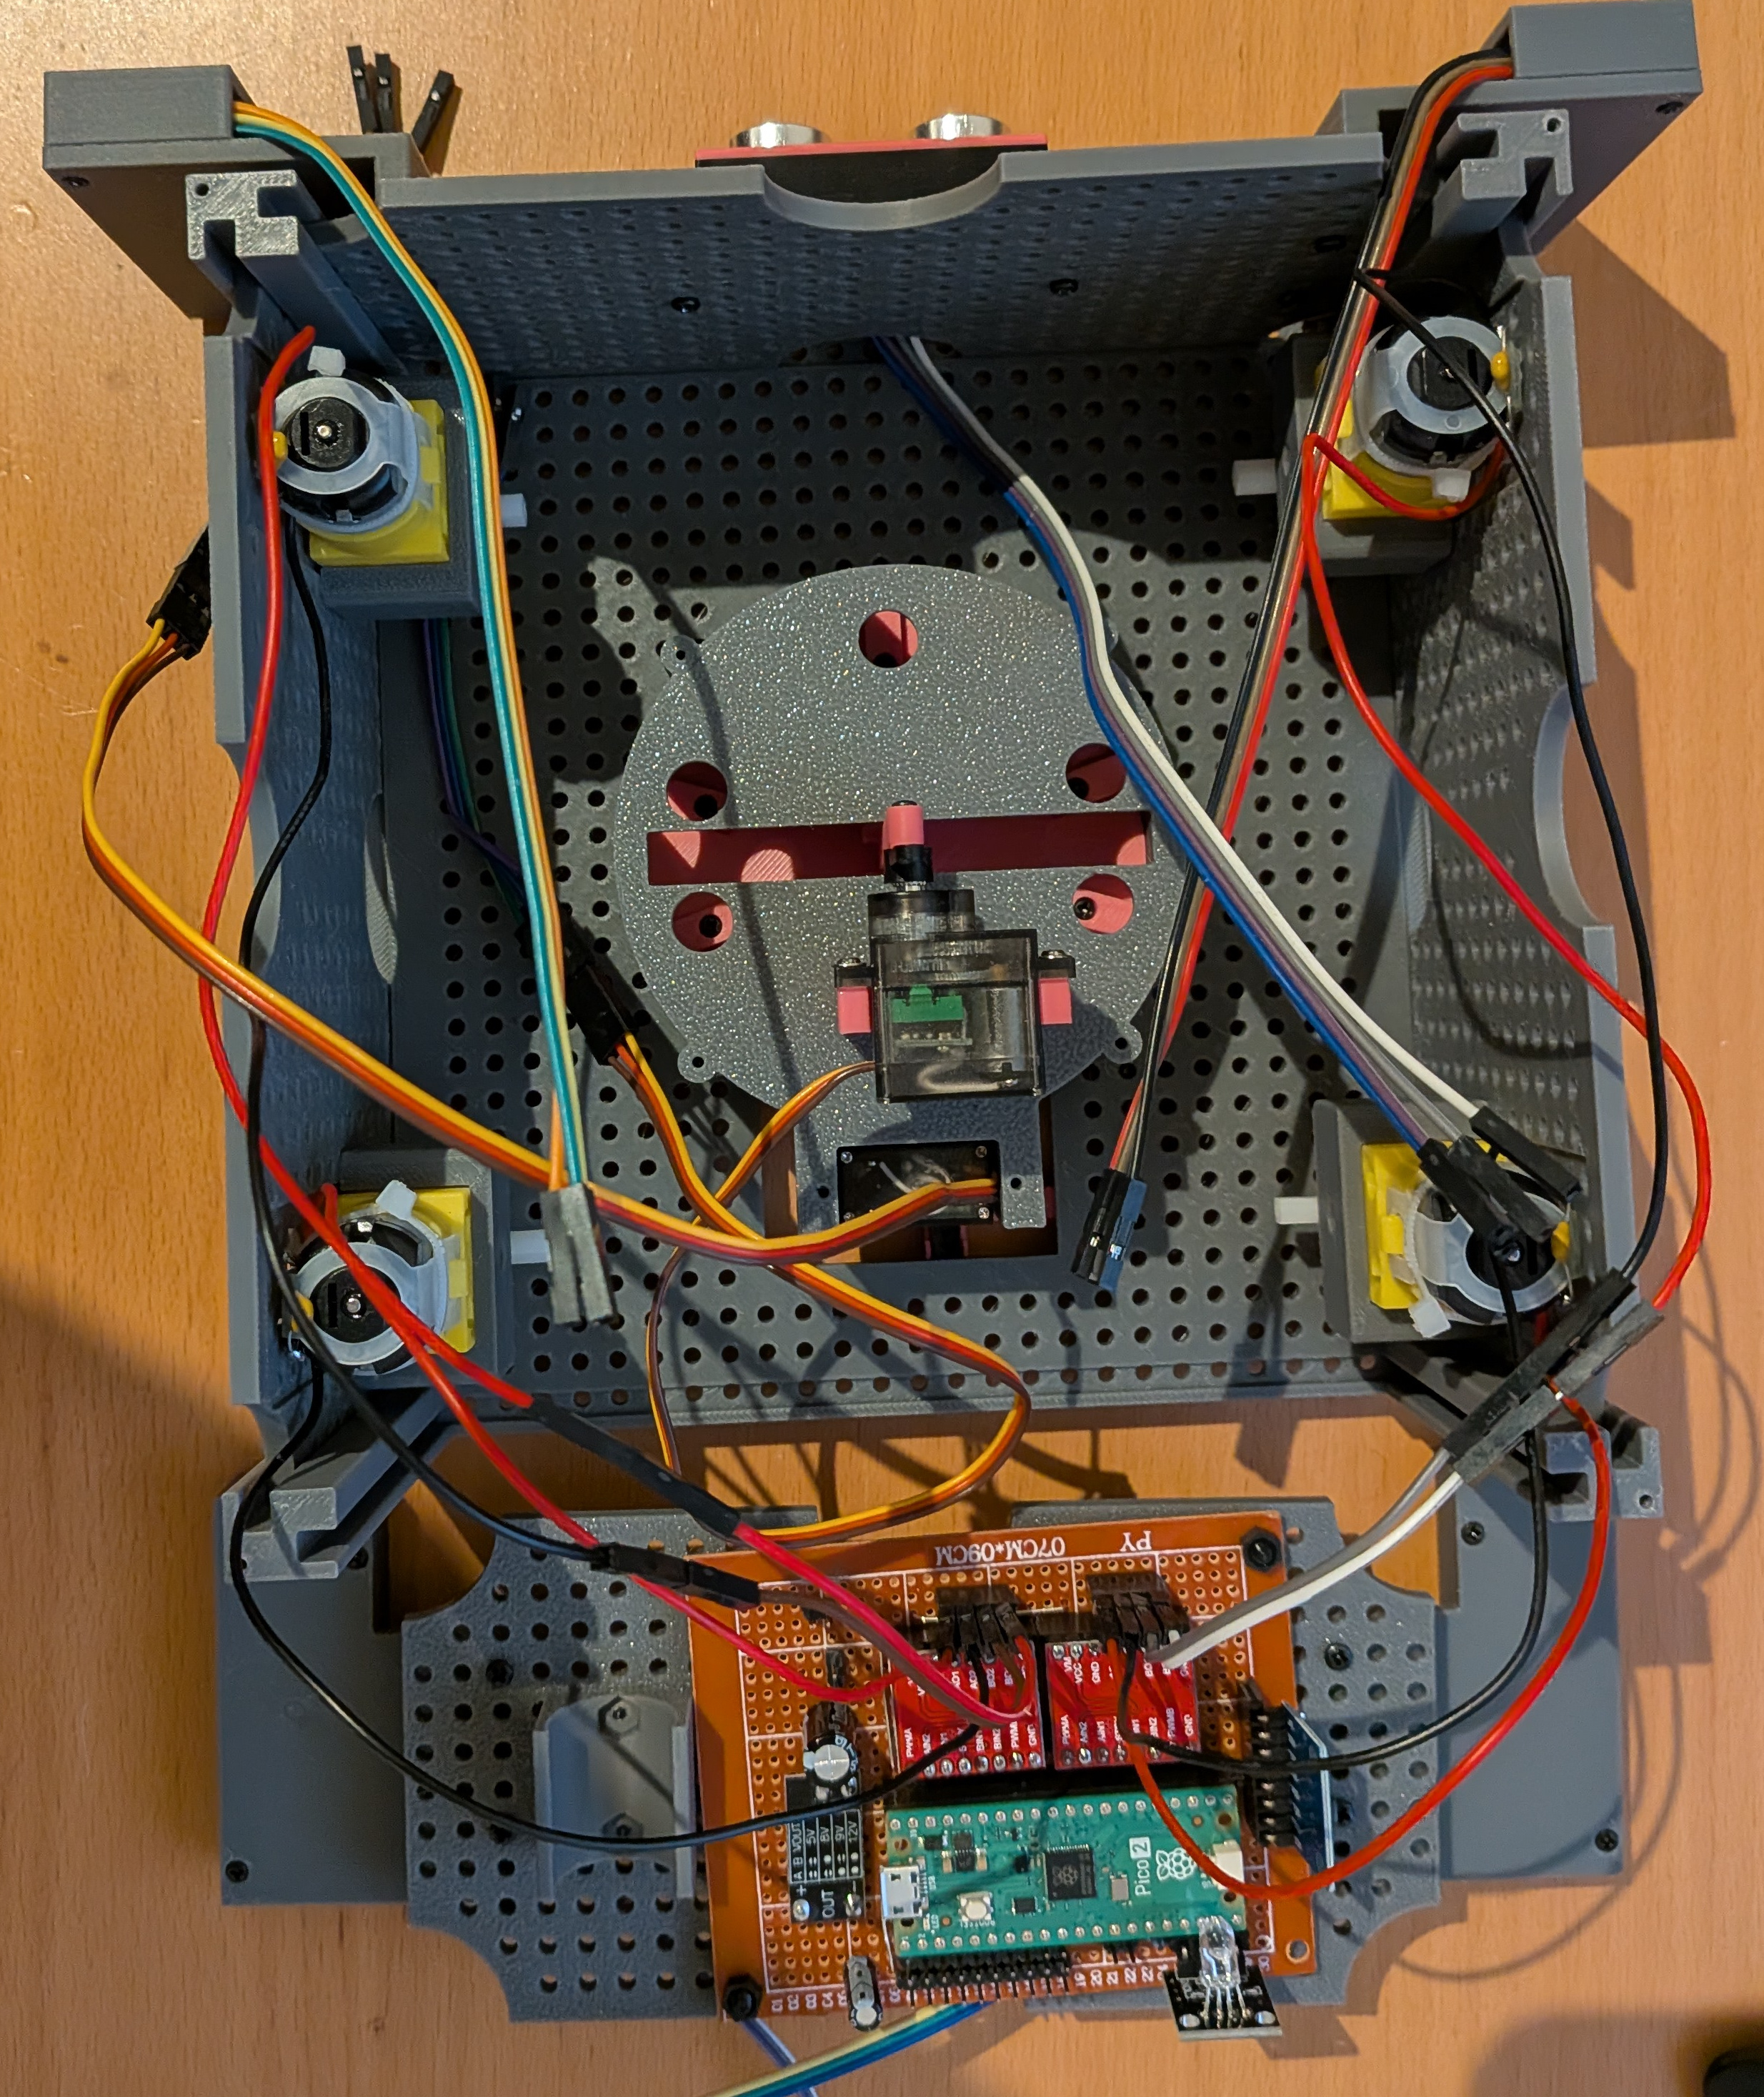
\includegraphics[scale=0.08]{montage_gereon/gesamt_montage/PXL_20260912_201400124.jpg}
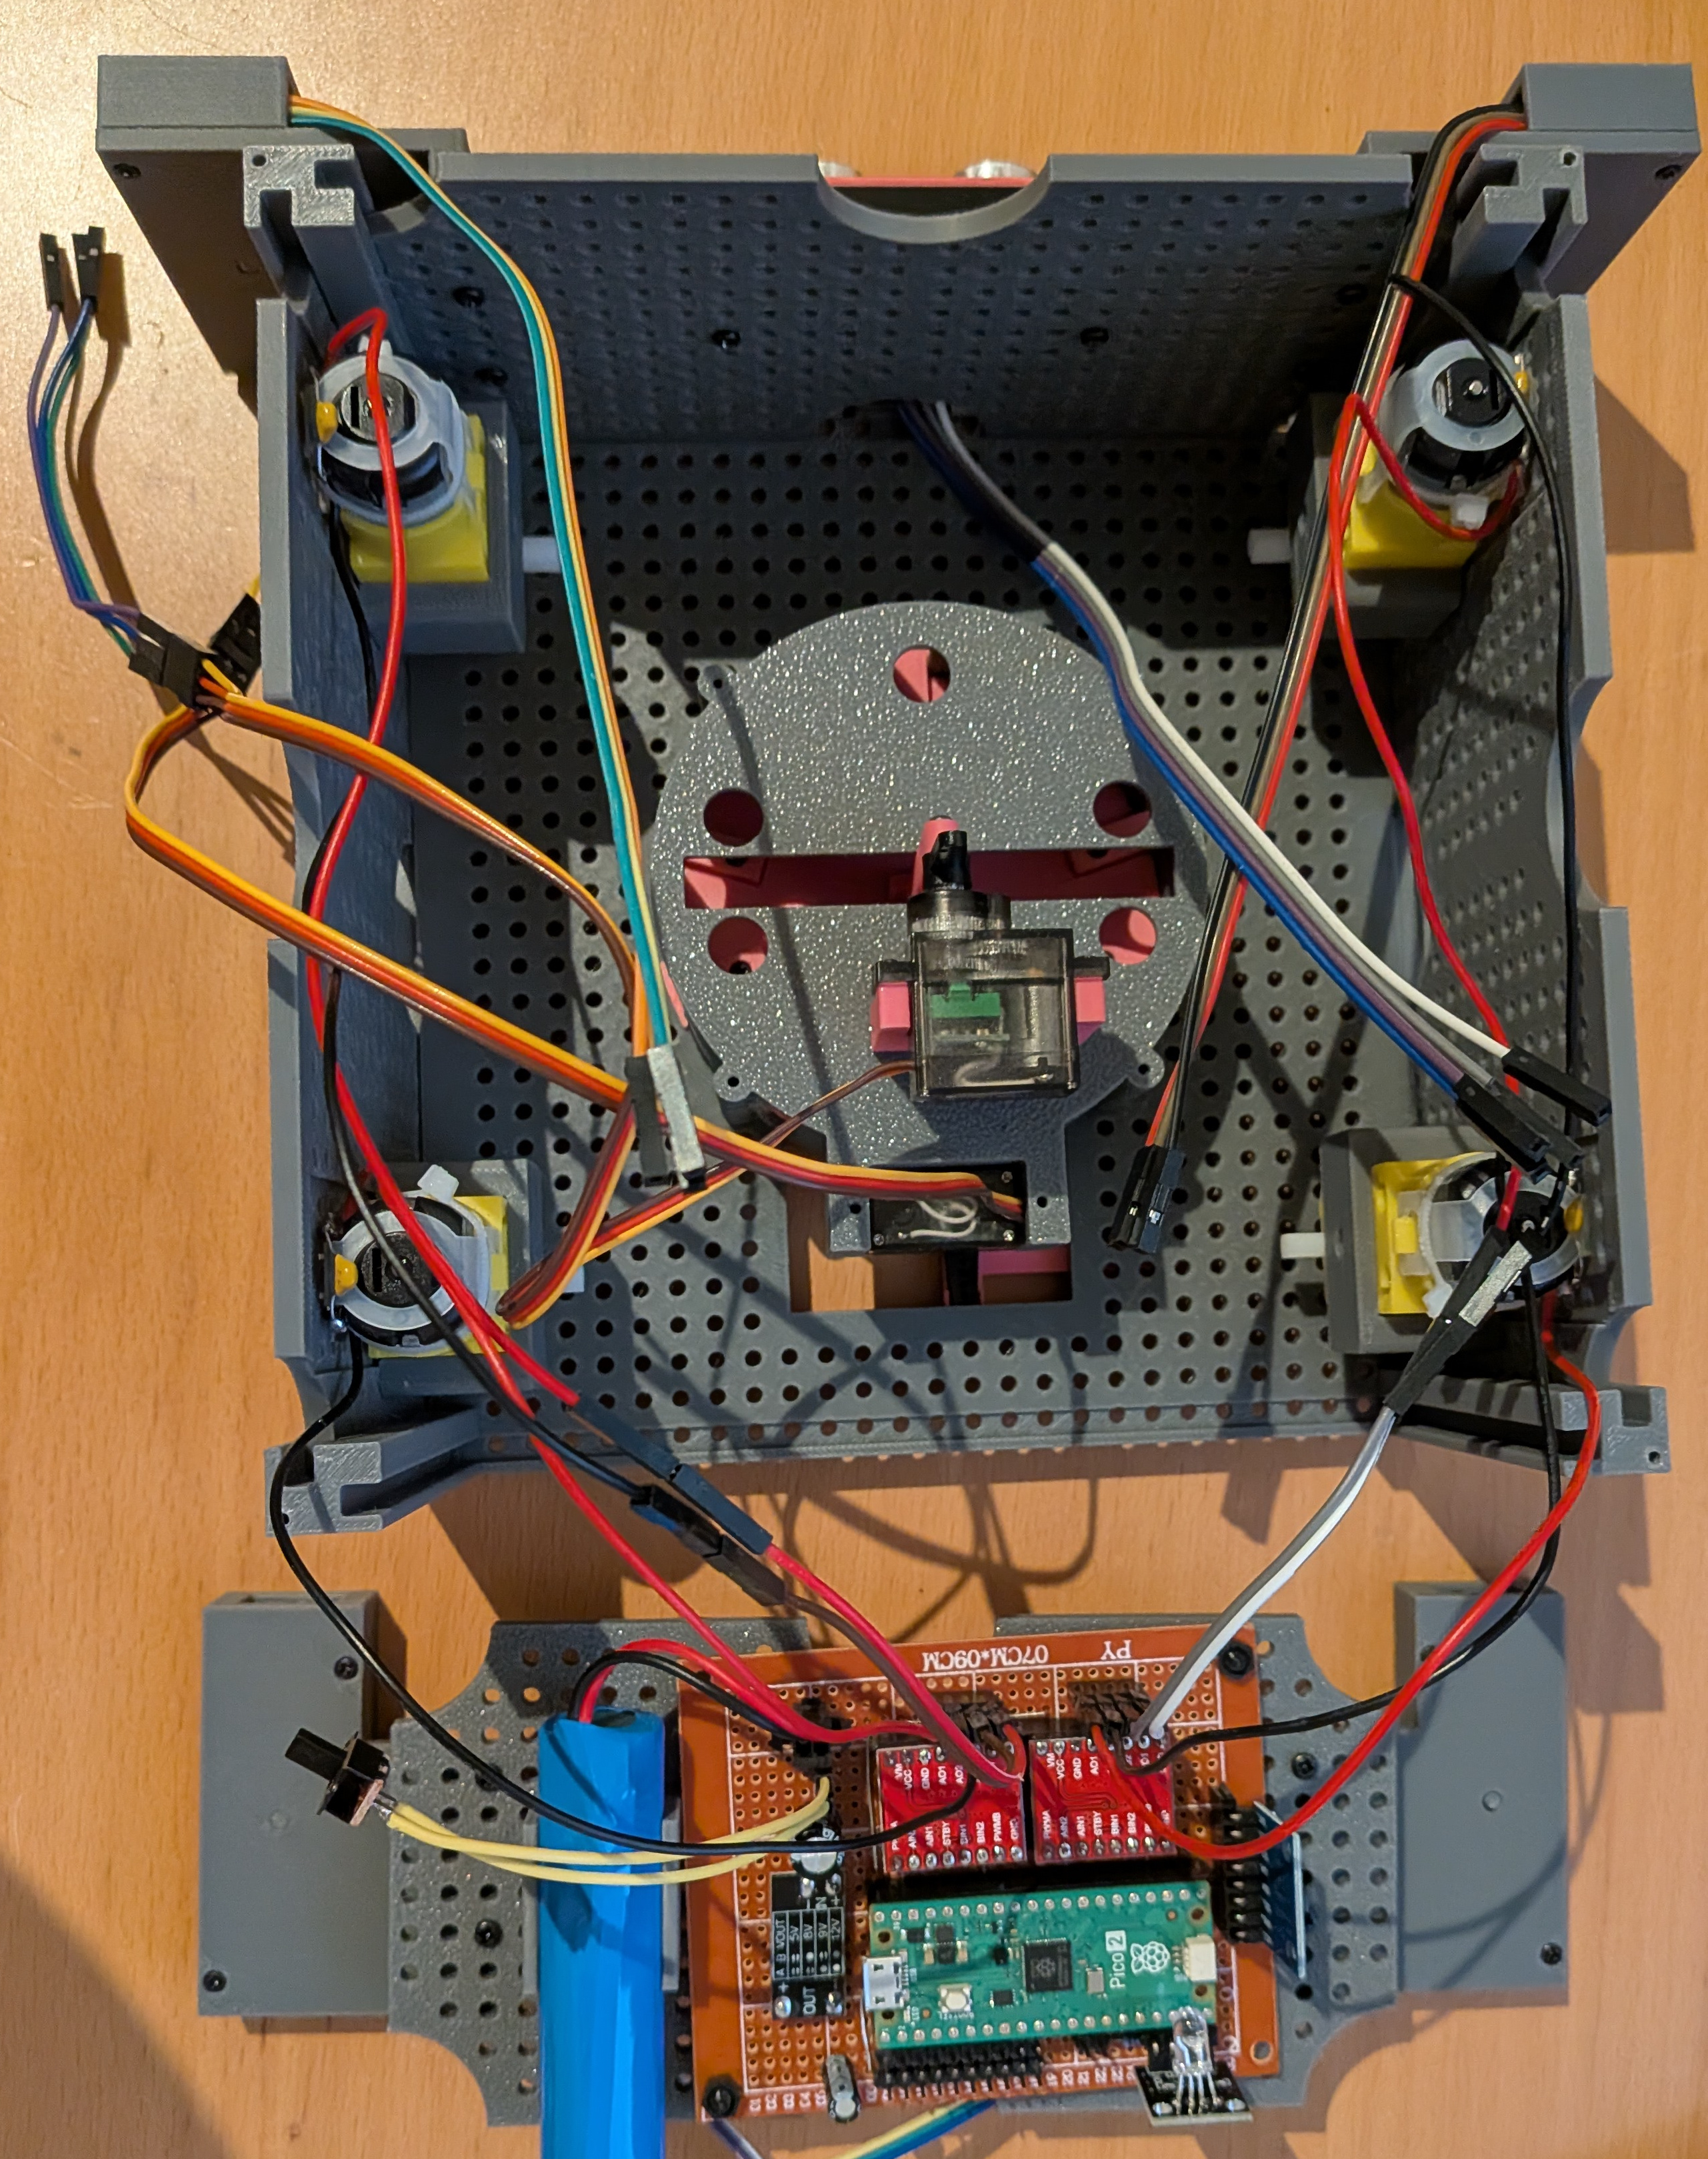
\includegraphics[scale=0.08]{montage_gereon/gesamt_montage/PXL_20260912_201453578.jpg}











\subsection{Schließen des Chassis}

TODO






\end{document}
